\documentclass[11pt,twoside]{report}
\usepackage{vdmlisting}
\usepackage{multicol}
\usepackage{pict2e}

\newcommand{\lbparen}{%
  \mathopen{%
    \sbox0{$()$}%
    \setlength{\unitlength}{\dimexpr\ht0+\dp0}%
    \raisebox{-\dp0}{%
      \begin{picture}(.32,1)
      \linethickness{\fontdimen8\textfont3}
      \roundcap
      \put(0,0){\raisebox{\depth}{$($}}
      \polyline(0.32,0)(0,0)(0,1)(0.32,1)
      \end{picture}%
    }%
  }%
}

\newcommand{\rbparen}{%
  \mathclose{%
    \sbox0{$()$}%
    \setlength{\unitlength}{\dimexpr\ht0+\dp0}%
    \raisebox{-\dp0}{%
      \begin{picture}(.32,1)
      \linethickness{\fontdimen8\textfont3}
      \roundcap
      \put(-0.08,0){\raisebox{\depth}{$)$}}
      \polyline(0,0)(0.32,0)(0.32,1)(0,1)
      \end{picture}%
    }%
  }%
}


\usepackage{color}        
\usepackage{alltt}  
\usepackage{hyperref}
\usepackage{amsmath}
\usepackage{unicode-math}
\usepackage{xcolor}
\usepackage{listings}
\usepackage{color}
\usepackage[toc,page]{appendix}
\usepackage{soul}
\sethlcolor{lightgray}
\lstdefinelanguage{Velocity}{
  keywords={\$Isa, true, false, \#foreach, \#if, \#end, null, \#else, \#elseif, \$node, \#, \#\#},
  keywordstyle=\color{orange}\bfseries,
  ndkeywords={\.trans, \\\<, \>},
  ndkeywordstyle=\color{gray}\bfseries,
  identifierstyle=\color{gray},
  sensitive=false,
  comment=[l]{\#},
  morecomment=[s]{\\<}{>},
  commentstyle=\color{blue}\ttfamily,
}

\lstdefinelanguage{Isabelle}{
  keywords={\\\<and\>, true, false, \#foreach, \#if, \#end, null, \#else, \#elseif, \$node, type_synonym, definition, where, abbreviation, record},
  keywordstyle=\color{blue}\bfseries,
  ndkeywords={\.trans, \\\<, \>},
  ndkeywordstyle=\color{pink}\bfseries,
  identifierstyle=\color{black},
  sensitive=false,
  comment=[l]{//},
  morecomment=[s]{\\<}{>},
  commentstyle=\color{black}\ttfamily,
  stringstyle=\color{purple}\ttfamily,
  morestring=[b]',
  morestring=[b]"
}

\definecolor{dkgreen}{rgb}{0,0.6,0}
\definecolor{gray}{rgb}{0.5,0.5,0.5}
\definecolor{mauve}{rgb}{0.58,0,0.82}

\lstset{frame=tb,
  language=Java,
  aboveskip=3mm,
  belowskip=3mm,
  showstringspaces=false,
  columns=flexible,
  basicstyle={\small\ttfamily},
  numbers=none,
  numberstyle=\tiny\color{gray},
  keywordstyle=\color{orange},
  commentstyle=\color{dkgreen},
  stringstyle=\color{mauve},
  breaklines=true,
  breakatwhitespace=true,
  tabsize=3
}
\NewDocumentCommand{\codeword}{v}{%
\texttt{\textcolor{cyan}{#1}}%
}
\newcommand{\syntaxNULL}[1]{\textcolor[rgb]{0.0,0.0,0.0}{#1}}
\newcommand{\syntaxCOMMENTA}[1]{\textcolor[rgb]{0.8,0.0,0.0}{#1}}
\newcommand{\syntaxCOMMENTB}[1]{\textcolor[rgb]{1.0,0.5176470588235295,0.0}{#1}}
\newcommand{\syntaxCOMMENTC}[1]{\textcolor[rgb]{0.4,0.0,0.8}{#1}}
\newcommand{\syntaxCOMMENTD}[1]{\textcolor[rgb]{0.8,0.4,0.0}{#1}}
\newcommand{\syntaxDIGIT}[1]{\textcolor[rgb]{1.0,0.0,0.0}{#1}}
\newcommand{\syntaxFUNCTION}[1]{\textcolor[rgb]{0.6,0.4,1.0}{#1}}
\newcommand{\syntaxINVALID}[1]{\colorbox[rgb]{1.0,1.0,0.8}{\textcolor[rgb]{1.0,0.0,0.4}{#1}}}
\newcommand{\syntaxKEYWORDA}[1]{\textcolor[rgb]{0.0,0.4,0.6}{\textbf{#1}}}
\newcommand{\syntaxKEYWORDB}[1]{\textcolor[rgb]{0.0,0.6,0.4}{\textbf{#1}}}
\newcommand{\syntaxKEYWORDC}[1]{\textcolor[rgb]{0.0,0.6,1.0}{\textbf{#1}}}
\newcommand{\syntaxKEYWORDD}[1]{\textcolor[rgb]{0.4,0.8,1.0}{\textbf{#1}}}
\newcommand{\syntaxLABEL}[1]{\textcolor[rgb]{0.00784313725490196,0.7254901960784313,0.00784313725490196}{#1}}
\newcommand{\syntaxLITERALA}[1]{\textcolor[rgb]{1.0,0.0,0.8}{#1}}
\newcommand{\syntaxLITERALB}[1]{\textcolor[rgb]{0.8,0.0,0.8}{#1}}
\newcommand{\syntaxLITERALC}[1]{\textcolor[rgb]{0.6,0.0,0.8}{#1}}
\newcommand{\syntaxLITERALD}[1]{\textcolor[rgb]{0.4,0.0,0.8}{#1}}
\newcommand{\syntaxMARKUP}[1]{\textcolor[rgb]{0.0,0.0,1.0}{#1}}
\newcommand{\syntaxOPERATOR}[1]{\textcolor[rgb]{0.0,0.0,0.0}{\textbf{#1}}}

\newcommand{\gutter}[1]{\textcolor[rgb]{0,0,0}{{|}#1}}
\newcommand{\gutterH}[1]{\textcolor[rgb]{1,0,0}{{|}#1}}

\definecolor{bgcolor}{rgb}{1.0,1.0,1.0}
\newsavebox{\opencurlybracket}%
\newsavebox{\closecurlybracket}%
\newsavebox{\lessthan}%
\newsavebox{\greaterthan}%
\newsavebox{\dollarbox}%
\newsavebox{\underscorebox}%
\newsavebox{\andbox}%
\newsavebox{\hashbox}%
\newsavebox{\backslashbox}%
\newsavebox{\atbox}%
\newsavebox{\percentbox}%
\newsavebox{\hatbox}%
\setbox\opencurlybracket=\hbox{\verb.{.}%
\setbox\closecurlybracket=\hbox{\verb.}.}%
\setbox\lessthan=\hbox{\verb.<.}%
\setbox\dollarbox=\hbox{\verb.$.}%
\setbox\underscorebox=\hbox{\verb._.}%
\setbox\andbox=\hbox{\verb.&.}%
\setbox\hashbox=\hbox{\verb.#.}%
\setbox\atbox=\hbox{\verb.@.}%
\setbox\backslashbox=\hbox{\verb.\.}%
\setbox\greaterthan=\hbox{\verb.>.}%
\setbox\percentbox=\hbox{\verb.\%.}%
\setbox\hatbox=\hbox{\verb.^.}%
\def\urltilda{\kern -.15em\lower .7ex\hbox{\~{}}\kern .04em}

\def\vdmlisting{\texttt{vdmlisting}}
\def\envvdmsl{\texttt{vdmsl}}
\usepackage{color}
\definecolor{dkgreen}{rgb}{0,0.6,0}
\definecolor{gray}{rgb}{0.5,0.5,0.5}
\definecolor{mauve}{rgb}{0.58,0,0.82}
\usepackage[citestyle=alphabetic,bibstyle=authortitle]{biblatex}
\addbibresource{Dissertation.bib}
\usepackage[utf8]{inputenc}
\usepackage{graphicx}
\usepackage[a4paper,width=150mm,top=25mm,bottom=25mm]{geometry}
\graphicspath{ {images/} }
\usepackage{fancyhdr}
\pagestyle{fancy}
\fancyhead{}
\fancyhead[RO,LE]{Creating a tool for the translation of VDM to Isabelle HOL}
\fancyfoot{}
\fancyfoot[LE,RO]{\thepage}
\fancyfoot[LO,CE]{\leftmark}
\fancyhead[LE,LO]{Jamie Simm}
\title{
{Creating a tool for the translation of VDM to Isabelle HOL}\\
{\vspace{0.5cm}}
{\large BSc Computer Science}\\
{\vspace{0.5cm}}
{\large Newcastle University}\\
{\vspace{0.5cm}}
{\large Project Supervisor Dr Leonardo J.S Freitas}\\
{\vspace{3cm}}
{\small Word count : 13751 in text, 245 outside text.}\\
{\vspace{2.5cm}}
{
\includegraphics[width=5cm, height=2cm ]{newcastle.jpg}}
}
\author{Jamie Simm}
\date{2019}

\begin{document}
\maketitle

\chapter*{Abstract}
This dissertation aims to explain and describe the implementation of and need for a VDM (Vienna Development Method) to Isabelle HOL (Higher Order Logic) translation tool. The tool is applied to a VDM model of the POLAR organ persufflation machine's alarm system. As Isabelle theories can be proven mathematically by the modeller, it is hoped that this tool will be useful in the verification of software by eliminating the need for manual VDM to Isabelle translation.
\chapter*{Declaration}
I declare that this dissertation represents my own work except where otherwise stated. The length of this document is only so large for its code snippets and figures, the majority of which take up a considerable amount of the page. Excluding them, this document would approximately measure thirty pages in length. 

\chapter*{Acknowledgments}
I would like to thank my supervisor, Dr Leo Freitas: for guiding me toward the project of developing this tool, which I have thoroughly enjoyed; for introducing me to the world of formal specification, Isabelle and VDM; and for fostering my interest in automated translation and proof tools. Secondly, I would like to thank Casper Thule Hansen of Aarhus University, Denmark, for setting up the environment upon which this tool was built and teaching me how to write transformation visitors. I believe that this project may not have been so successful without such an essential and flexible platform for it to be built upon. 

\tableofcontents

\chapter{Introduction}
\section{The POLAR machine and persufflation}
Organ preservation is a vital factor in the success and availability of allotransplantation\footnote{The transplantation of organs, tissue, or cells from a genetically distinct individual of the same species.} as a treatment for illness, conventional methods like Static Cold Storage (SCS) have a number of issues - advancements in this field could serve to transform medicine\parencite{Giwa2017}. One such issue is that SCS is incapable of sufficient oxygen delivery during preservation\parencite{Pappas2005}. The POLAR project aims to address this issue by designing a machine to automate another method of organ preservation, persufflation, which gives a far higher oxygen supply per gram of tissue. 

\section{Verifying the correctness of the machine to ensure reliability}
To achieve verification of the system we apply formal modelling techniques to its specification in order to derive an unambiguous representation of its components and its operation. For POLAR, this has been done by translating the machine's various alarm conditions into a VDM-SL model. VDM-SL is a formal modelling language, it allows the modeller to abstract the system into a mathematical representation, its syntax rules and semantics are so precisely defined that there is no room for disagreement about the model’s properties. This means that the POLAR VDM-SL model can be analysed using mathematical proof. In principal, we can prove that a program, in this case the alarm system, is correct with respect to its specification and prove that the POLAR VDM-SL model embodies a property such as safety - which is critical in a medical system. While VDM-SL has tools for generating proof obligations, it has no support for mathematical proof of those obligations.

One way to prove a VDM-SL model is to translate it into HOL\footnote{Higher order logic, essentially higher-order simple predicate logic, quantifies over an arbitrary number of nested sets i.e. where first-order logic quantifies only variables that range over individuals and second-order logic quantifies variables that range over both individuals and sets; third-order also quantifies over sets of sets etc. Higher Order Logic is a union of first, second third up to any number of $N$ nested sets.} so that it can then be proven using the proof assistant Isabelle, this is how the POLAR model will be proven. Ordinarily, translation is done manually, this can be an arduous process for the modeller/prover who should only be concerned with the proof of the model rather than the process of translation. 

Currently, there exists an effort to create a tool that will automate translation so that the modeller/prover can focus their efforts on proof of the system, as this is the pertinent part of the verification process\parencite{VDM2ISAGit}. In its current state at the time of beginning this dissertation, the tool does not have the functionality to translate the POLAR model and can only translate integer basic types as well as arithmetic and predicate expressions. With more work, applying the automated translation tool to the POLAR model could save a considerable amount of time in its verification and work on proving the machine's alarm system mathematically could begin sooner and therefore be more thorough. Human errors made during manual translation would be removed, reducing the likelihood that the modeller wastes time proving an incorrect translation.

One viable important change is the aims and objectives. You can say you are part of the dev team for the translator. 

Also, understanding as an objective is a bit weak. I think you can say learn it to enable/create X. And rather than just Java visitor, it’s a Overture/VDm visitor (ie more complex). There is also the AST, and the overall tool framework.

\section{Aims and Objectives} 
\subsection{Aim}
The aim of this dissertation is to extend the current VDM-SL to Isabelle translation tool so that it can translate more components of the POLAR model.
\subsection{Objectives} \label{objectives}
\begin{itemize}
	\item Learn the Java visitor design pattern and its implementation with adaptor classes and cases in Overture/VDM, in order to create the Java visitors that make AST transformations which enable translation.
	\item Learn the architecture of VDM's modules and the AST as well as the existing tool framework in order to inform development of further tool functionality.
	\item Apply the translator to the POLAR model.
\end{itemize}

\section{Document structure}
The following document will: provide background by explaining and discussing the area/domain that the project affects and explores; clarify existing works on the translation tool; present the implementation of my contribution to the tool, with a description of implementation issues and headlines; present the results of the tools development, as well as the results of its application to the POLAR example, and reflect upon the development process; conclude this dissertation with a proposal of future work, description of the impact of this project, a measure of success against proposed aims and objectives and an analysis of the project's complexity.


\chapter{Background}
This section attempts to explain and discuss the key concepts that are the foundation of this project: the POLAR organ persufflation machine and its formal model in VDM; mathematically proving a model in Isabelle and implementing a tool to translate a VDM model into Isabelle HOL; an outline of the problems that this dissertation aims to tackle, as well as the proposed solutions to those problems.

\section{Persufflation}
Organ persufflation is a method for organ preservation in which a donor organ is submerged in a cold preservation solution, a catheter\footnote{A flexible tube inserted through a narrow opening into a body cavity.} is then inserted into the vasculature\footnote{The arrangement of blood vessels in the body, or within an organ.} of the organ and oxygen is pumped into the organ through the catheter, thereby oxygenating\footnote{Supply, treat, charge, or enrich with oxygen.} the organ, see Fig\ref{fig:Persufflation}.\begin{figure}
        \center{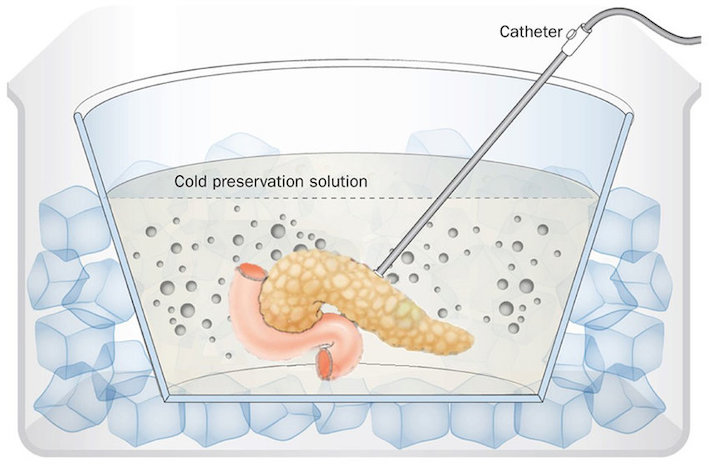
\includegraphics[width=\textwidth]
        {Images/Persufflation.jpeg}}
        \caption{\label{fig:Persufflation} Persufflation \parencite{Dholakia2018}}
      \end{figure} Through this method, more oxygen is delivered to the organ than the other most popular methods and by doing so preservation period can be extended by up to 48-72 hours\parencite{Suszynski2013}. 

However, Persufflation is a delicate process. Oxygen flow, temperature and pressure both inside and outside of the organ must be kept within a precise margin; slightly anomalous variations in any of these variables, could result in damage to the organ. 
Until now, humans have controlled these variables manually: typically, an alarm will sound if a variable exceeds its boundary and an attendant will adjust the value by hand. This method is not precise enough under such safety critical circumstances as human error may result in damage to the organ pre-transplant or failure of the organ post-transplant, due to poor condition.

Through software, the POLAR project's persufflation machine would enable effective, long term persufflation by removing the human element. By exploiting the speed, precision and accuracy of a computer system, POLAR hopes to be able to control these variables with high precision and within a minuscule margin of error. However, as is the nature of software of such complexity, the alarm system that informs changes to variables may be rife with errors, with high potential for unintended behaviour\parencite{JamiaOCW154}. In a safety critical system such as this, it is imperative that software components do not malfunction.


\section{POLAR System Complexity}
The POLAR machine is a Cyber-Physical System - collaborating computational elements controlling physical entities, which interact with humans and their environment. For the sake of keeping safety in mind, it is important to note that the software that will be developed for POLAR is part of a system - a combination of interacting elements organized to achieve one or more stated purposes\parencite{walden_roedler_forsberg_hamelin_shortell_2007}. As such, the system will have several dimensions to take into account - building complexity. Physical variables such as external and internal pressure, temperature, atmospheric composition, movement and more. Also computational variables such as security protocols, fail safes, varying software; Human variables, how will the machine be handled, used, what errors may humans introduce into the system? 

Specifically, human contribution is arguably the central source of error and complexity in a system. Separate discipline-specific development processes result in components being developed in a disjointed manner. In the case of POLAR, software is developed separate to the hardware, a machine engineer is not able to know precisely how their chip's resources will be handled by kernel processes written by the operating system developer, and so they are unable to understand which features might cause error, which limitations the software will have. All of this risks late discovery of defects, namely at the integration stage, when it is highly cumbersome to go back. 

\section{Modelling}
The best way to bridge the gap between varying components, development teams, dimensions of the system, is to create a model of the system, an abstraction of all of these variables together in one unambiguous representation so that the variables of the system can be tested and scrutinised as a whole, their interaction monitored and alterations made where error is found. Models allow us to explore a design space before we build, and physically integrate, the components within it. Interactions are modelled as contracts, assumptions and guarantees of what will or should happen rather than how. As an architect models a structure to smaller scale before it is built - so is a software and hardware system modelled before it is integrated and implemented. This provides evidence for trust, reduces risk of bugs and can even identify improvements to the current design. In POLAR, a system that will someday contribute to human well-being, it is easy to see how an optimal design and faster development will be beneficial. For an increasing amount of software, this model takes the form of a formal specification.

\section{Formal Specification}
Formal specifications are used to describe a system, analyse its behaviour and to aid in its design by verifying key properties of interest through rigorous and effective reasoning tools\parencite{FORMAL1}\parencite{FORMAL2}. These specifications are formal in the sense that they have a syntax, their semantics fall within one domain, and they are able to be used to infer useful information\parencite{Lamsweerde2000}.\parencite{wikiFS} Ordinarily, a formal specification of a system goes no further than a UML diagram of its components and mostly all projects have some form of it. This is a good first approximation, but it is imprecise. For safety critical systems, a mathematical, unambiguous abstraction of the system, which states the effect of computation, is the only acceptable level of specification. A mathematical representation can be analysed, altered and proven using deduction and reasoning techniques - and therefore, so can the design of the system with respect to its specification. A mathematical specification is encoded in an appropriate formal modelling programming language, for POLAR this is VDM-SL.


\section{Vienna Development Method Specification Language (VDM-SL)}
Though readers of this dissertation might already be familiar with VDM, a brief overview of the language is necessary to provide motivation for this project. VDM is a state-based modelling language which allows the modeller to formally specify structure, behaviour and logical constraints. The Vienna Development Method (VDM) was established in the 1970's originating from IBM Laboratory, Vienna. The language has syntax to represent mathematical representation of a specification. Mathematical constructs including, sets, sequences and integers, to name a small few, define types of data that are maintained and transformed in the system. How this data is represented, what restrictions are placed on the data, represented as invariants on types and values, and what data forms the persistent state of the system, define its data set. Behaviour of the system is encoded as functions that represent functionality, and as operations which modify its persistent state. Pre and post conditions for operations and functions are purposeful in both restricting and checking their operation. Errors in the model identify errors in the specification of the system, the specification can then be altered, and the design improved to eliminate errors before the new specification is written in VDM-SL again so that all of this can be repeated. Many iterations of this - model, check, alter, model again - cycle incrementally identify and eliminate errors until none, or as few as possible within a reasonable threshold, can be found.



\subsection{VDM-SL Example, Alarm System}
Below, VDM code represents the alarm system for a nuclear power plant reactor. Experts are paged when certain variables' values cross safe boundaries. Certain experts are on shift at certain times and paging is decided based on period of time over boundaries as well as other important factors such as an expert’s qualification.


\begin{vdmsl}[label=lst:AlarmSL.vdmsl,caption=Types of data used in the alarm system in VDM-SL]
types

Schedule = map Period to set of Expert;

Period = token;

Expert :: expertid : ExpertId
quali : set of Qualification
inv ex == ex.quali <> {};

ExpertId = token;
Qualification = <Elec> | <Mech> | <Bio> | <Chem>;
Alarm :: alarmtext : seq of char
quali : Qualification;
\end{vdmsl}

Above, an invariant on the Expert type is defined to ensure that the expert does not have an empty set of qualifications i.e. the expert is qualified, and their qualifications are recorded.

\begin{vdmsl}[label=lst:AlarmSL.vdmsl,caption=Alarm system's values in VDM-SL]
values
 
  p1:Period = mk_token("Monday day");
  ps : set of Period = {p1,p2,p3,p4,p5};

  eid8:ExpertId = mk_token(190);
  
  e1:Expert = mk_Expert(eid1,{<Elec>});
  exs : set of Expert = {e1,e2,e3,e4,e5,e6,e7,e8};
\end{vdmsl}

Some of the values in the system are shown above. A set of experts is created, one such expert having a particular id and electrical qualification.

\begin{vdmsl}[label=lst:AlarmSL.vdmsl,caption=An alarm system function in VDM-SL which takes a set of experts\, a qualification and returns a boolean value.]
functions
  QualificationOK: set of Expert * Qualification -> bool
  QualificationOK(exs2,reqquali) ==
    exists ex in set exs2 & reqquali in set ex.quali;
\end{vdmsl}
\hfill\break
\hfill\break
\begin{vdmsl}[label=lst:AlarmSL.vdmsl,caption=Alarm system's persistent state in VDM-SL\, t he state is represented as a record type with the important persistent data as fields\, here schedule and alarms.]
state Plant of
schedule : Schedule
alarms : set of Alarm

\end{vdmsl}

\begin{vdmsl}[label=lst:AlarmSL.vdmsl,caption=Operations on the state of the alarm system in VDM-SL\, operations manipulate data stored in the persistent state and mimic the operation of the system.]
operations

NumberOfExperts: Period ==> nat
NumberOfExperts(peri) == is not yet specified
pre peri in set dom schedule;

ExpertIsOnDuty: Expert ==> set of Period

ExpertIsOnDuty(ex) == is not yet specified;

ExpertToPage: Alarm * Period ==> Expert

ExpertToPage(a,peri) == is not yet specified;
\end{vdmsl}

\section{Isabelle Translation}
VDM provides an unambiguous mathematical representation of the system, \textbf{however it does not provide any support for mathematical proof of the specification}. Mathematically proving or disproving correctness of the VDM model and its intended algorithms, allows us to say without doubt that they are correct with respect to their formal specification. Isabelle allows us to write code contracts in Higher Order Logic statements and provides an automated theorem proving assistant to prove them. Code contracts are assumptions and guarantees in the model, features written as VDM constructs. Contracts include but are not limited to: \begin{itemize}
  \item Properties that always hold (i.e. invariants).
  \item Assumptions (pre conditions) and commitments (post conditions).
  \item Proof obligations of interest such as satisfiability\footnote{A logical check to verify that operations are feasible} and reification\footnote{Do representations of the data in the system agree with one another, are they compatible?}, which if proved would establish the consistency of the model.
  \item Proof obligations (POs) of what correctness means, verifying that we have built the correct model.
  \item Sanity checks on functionality, validating that the model has been built correctly.
\end{itemize}
Isabelle is a functional programming language, constructs are represented as fields and curried functions, all collected together in a \syntaxKEYWORDA{theory}, \syntaxKEYWORDA{.thy}, file. A theory is a named collection of types, functions, and theorems, much like a module in a programming language or a specification in a specification language like VDM. Isabelle contains a theory file \syntaxKEYWORDA{"Main"}, which is a union of all the basic, predefined theories like arithmetic, lists, sets, etc. which are used by the automated theorem prover to inform proof assistants. Below, a module \syntaxLITERALA{"VDMToolkit"}\footnote{VDMToolkit is written and maintained by Dr Leonardo Jose Simoes Freitas. Newcastle University.} is included in the imports. This is very important in the VDM to Isabelle translation steps as, similar to \syntaxKEYWORDA{"Main"}, it provides type-checked VDM constructs with pre, post conditions and invariants for VDM types like VDMNat1 and VDMSet, as VDM represents these things differently to Isabelle.

To use Isabelle to prove a model, that model must first be translated from VDM into Isabelle HOL. For the above example, translations are below.

\hfill\break
\hfill\break
\ttfamily
\syntaxNULL{}\gutter{\ \ \ \ 1{|}\ }\syntaxKEYWORDA{theory}{\ }Alarm\hspace*{\fill}\\
\gutter{\ \ \ \ 2{|}\ }\syntaxKEYWORDB{imports}{\ }\syntaxLITERALA{"../../lib/VDMToolkit"}\hspace*{\fill}\\
\gutter{\ \ \ \ 3{|}\ }\syntaxKEYWORDB{begin}\hspace*{\fill}\\
\gutter{\ \ \ 42{|}\ }{\ }{\ }\hspace*{\fill}\\
\gutter{\ \ \ 42{|}\ }{\ }{\ }\hspace*{\fill}\\
\gutter{\ \ \ \ 7{|}\ }\syntaxKEYWORDA{type\usebox{\underscorebox}synonym}{\ }Period{\ }{\ }{\ }\syntaxOPERATOR{=}{\ }VDMToken\hspace*{\fill}\\
\gutter{\ \ \ 14{|}\ }\syntaxKEYWORDA{definition}\hspace*{\fill}\\
\gutterH{\ \ \ 15{|}\ }{\ }{\ }inv\usebox{\underscorebox}Period{\ }\syntaxOPERATOR{::}{\ }\syntaxLITERALA{"Period{\ }⇒{\ }𝔹"}\hspace*{\fill}\\
\gutter{\ \ \ 16{|}\ }{\ }{\ }\syntaxKEYWORDB{where}\hspace*{\fill}\\
\gutter{\ \ \ 17{|}\ }{\ }{\ }\syntaxLITERALA{"inv\usebox{\underscorebox}Period{\ }≡{\ }inv\usebox{\underscorebox}True"}\hspace*{\fill}\\
\gutter{\ \ \ 18{|}\ }{\ }{\ }\hspace*{\fill}\\
\gutter{\ \ \ 19{|}\ }\syntaxKEYWORDA{type\usebox{\underscorebox}synonym}{\ }ExpertId{\ }\syntaxOPERATOR{=}{\ }VDMToken\hspace*{\fill}\\
\gutterH{\ \ \ 20{|}\ }\hspace*{\fill}\\
\gutter{\ \ \ 21{|}\ }\syntaxKEYWORDA{datatype}{\ }Qualification{\ }\syntaxOPERATOR{=}{\ }Elec{\ }\syntaxOPERATOR{|}{\ }Mech{\ }\syntaxOPERATOR{|}{\ }Bio{\ }\syntaxOPERATOR{|}{\ }Chem\hspace*{\fill}\\
\gutter{\ \ \ 22{|}\ }\hspace*{\fill}\\
\gutter{\ \ \ 23{|}\ }\syntaxKEYWORDA{definition}\hspace*{\fill}\\
\gutter{\ \ \ 24{|}\ }{\ }{\ }inv\usebox{\underscorebox}Qualification{\ }\syntaxOPERATOR{::}{\ }\syntaxLITERALA{"Qualification{\ }⇒{\ }𝔹"}\hspace*{\fill}\\
\gutterH{\ \ \ 25{|}\ }{\ }{\ }\syntaxKEYWORDB{where}\hspace*{\fill}\\
\gutter{\ \ \ 26{|}\ }{\ }{\ }\syntaxLITERALA{"inv\usebox{\underscorebox}Qualification{\ }≡{\ }inv\usebox{\underscorebox}True"}\hspace*{\fill}\\
\gutter{\ \ \ 27{|}\ }{\ }{\ }\hspace*{\fill}\\
\gutter{\ \ \ 28{|}\ }\syntaxKEYWORDA{record}{\ }Alarm{\ }\syntaxOPERATOR{=}\hspace*{\fill}\\
\gutter{\ \ \ 29{|}\ }{\ }{\ }alarm\usebox{\underscorebox}alarmtext{\ }\syntaxOPERATOR{::}{\ }\syntaxLITERALA{"char{\ }VDMSeq"}{\ }{\ }\hspace*{\fill}\\
\gutterH{\ \ \ 30{|}\ }{\ }{\ }alarm\usebox{\underscorebox}quali{\ }{\ }{\ }{\ }{\ }\syntaxOPERATOR{::}{\ }Qualification\hspace*{\fill}\\
\gutter{\ \ \ 27{|}\ }{\ }{\ }\hspace*{\fill}\\
\gutter{\ \ \ 38{|}\ }\syntaxKEYWORDA{definition}\hspace*{\fill}\\
\gutter{\ \ \ 39{|}\ }{\ }{\ }inv\usebox{\underscorebox}Alarm{\ }\syntaxOPERATOR{::}{\ }\syntaxLITERALA{"Alarm{\ }⇒{\ }𝔹"}\hspace*{\fill}\\
\gutterH{\ \ \ 40{|}\ }{\ }{\ }\syntaxKEYWORDB{where}\hspace*{\fill}\\
\gutter{\ \ \ 41{|}\ }{\ }{\ }\syntaxLITERALA{"inv\usebox{\underscorebox}Alarm{\ }≡{\ }inv\usebox{\underscorebox}True"}\hspace*{\fill}\\
\gutter{\ \ \ 42{|}\ }{\ }{\ }\hspace*{\fill}\\
\gutter{\ \ \ 43{|}\ }\syntaxKEYWORDA{record}{\ }Expert{\ }\syntaxOPERATOR{=}\hspace*{\fill}\\
\gutter{\ \ \ 44{|}\ }{\ }{\ }expert\usebox{\underscorebox}expertid{\ }{\ }\syntaxOPERATOR{::}{\ }ExpertId\hspace*{\fill}\\
\gutterH{\ \ \ 45{|}\ }{\ }{\ }expert\usebox{\underscorebox}quali{\ }{\ }{\ }{\ }{\ }\syntaxOPERATOR{::}{\ }\syntaxLITERALA{"Qualification{\ }VDMSet"}\hspace*{\fill}\\
\gutter{\ \ \ 46{|}\ }{\ }{\ }\hspace*{\fill}\\
\gutter{\ \ \ 47{|}\ }\syntaxKEYWORDA{definition}\hspace*{\fill}\\
\gutter{\ \ \ 48{|}\ }{\ }{\ }inv\usebox{\underscorebox}Expert{\ }\syntaxOPERATOR{::}{\ }\syntaxLITERALA{"Expert{\ }⇒{\ }𝔹"}\hspace*{\fill}\\
\gutter{\ \ \ 49{|}\ }{\ }{\ }\syntaxKEYWORDB{where}\hspace*{\fill}\\
\gutterH{\ \ \ 50{|}\ }{\ }{\ }\syntaxLITERALA{"inv\usebox{\underscorebox}Expert{\ }e{\ }≡}\hspace*{\fill}\\
\gutter{\ \ \ 51{|}\ }\syntaxLITERALA{{\ }{\ }{\ }{\ }{\ }{\ }let{\ }eq{\ }={\ }(expert\usebox{\underscorebox}quali{\ }e){\ }in{\ }}\hspace*{\fill}\\
\gutter{\ \ \ 52{|}\ }\syntaxLITERALA{{\ }{\ }{\ }{\ }{\ }{\ }{\ }{\ }inv\usebox{\underscorebox}SetElems{\ }inv\usebox{\underscorebox}True{\ }eq{\ }∧}\hspace*{\fill}\\
\gutter{\ \ \ 53{|}\ }\syntaxLITERALA{{\ }{\ }{\ }{\ }{\ }{\ }{\ }{\ }eq{\ }≠{\ }\usebox{\opencurlybracket}\usebox{\closecurlybracket}"}\hspace*{\fill}\\
\gutter{\ \ \ 54{|}\ }\hspace*{\fill}\\
\gutter{\ \ \ 74{|}\ }\syntaxKEYWORDA{type\usebox{\underscorebox}synonym}{\ }Schedule{\ }\syntaxOPERATOR{=}{\ }\syntaxLITERALA{"Period{\ }⇀{\ }Expert{\ }set"}{\ }\hspace*{\fill}\\
\gutterH{\ \ \ 75{|}\ }{\ }{\ }\hspace*{\fill}\\
\gutter{\ \ \ 77{|}\ }\syntaxKEYWORDA{definition}\hspace*{\fill}\\
\gutter{\ \ \ 78{|}\ }{\ }{\ }inv\usebox{\underscorebox}Schedule{\ }\syntaxOPERATOR{::}{\ }\syntaxLITERALA{"Schedule{\ }⇒{\ }𝔹"}\hspace*{\fill}\\
\gutter{\ \ \ 79{|}\ }{\ }{\ }\syntaxKEYWORDB{where}\hspace*{\fill}\\
\gutterH{\ \ \ 80{|}\ }{\ }{\ }\syntaxLITERALA{"inv\usebox{\underscorebox}Schedule{\ }s{\ }≡{\ }}\hspace*{\fill}\\
\gutter{\ \ \ 81{|}\ }\syntaxLITERALA{{\ }{\ }{\ }{\ }{\ }{\ }inv\usebox{\underscorebox}Map{\ }inv\usebox{\underscorebox}Period{\ }(inv\usebox{\underscorebox}SetElems{\ }inv\usebox{\underscorebox}Expert){\ }s{\ }}\hspace*{\fill}\\
\gutter{\ \ \ 82{|}\ }\syntaxLITERALA{{\ }∧}\hspace*{\fill}\\
\gutter{\ \ \ 83{|}\ }\syntaxLITERALA{{\ }{\ }{\ }{\ }{\ }{\ }(∀{\ }exs1{\ }∈{\ }rng{\ }s{\ }.{\ }}\hspace*{\fill}\\
\gutter{\ \ \ 84{|}\ }\syntaxLITERALA{{\ }{\ }{\ }{\ }{\ }{\ }{\ }{\ }{\ }{\ }exs1{\ }≠{\ }\usebox{\opencurlybracket}\usebox{\closecurlybracket}{\ }∧}\hspace*{\fill}\\
\gutterH{\ \ \ 85{|}\ }\syntaxLITERALA{{\ }{\ }{\ }{\ }{\ }{\ }{\ }{\ }{\ }{\ }(∀{\ }ex1{\ }∈{\ }exs1{\ }.{\ }∀{\ }ex2{\ }∈{\ }exs1{\ }.{\ }}\hspace*{\fill}\\
\gutter{\ \ \ 86{|}\ }\syntaxLITERALA{{\ }{\ }{\ }{\ }{\ }{\ }{\ }{\ }{\ }{\ }{\ }{\ }{\ }{\ }ex1{\ }≠{\ }ex2{\ }⟶{\ }(expert\usebox{\underscorebox}quali{\ }ex1){\ }≠{\ }(expert\usebox{\underscorebox}quali{\ }ex2)))"}\hspace*{\fill}\\
\gutter{\ \ \ 87{|}\ }{\ }{\ }\hspace*{\fill}\\
\gutter{\ \ 716{|}\ }\syntaxKEYWORDB{end}\hspace*{\fill}\\
\hfill\break
\hfill\break
\rmfamily
The translation 'recipe' detailing the general method for translation will be detailed in the Implementation section of this document later, see \ref{itr}. It is evident that translations might become very intricate and cumbersome for more complex models, human error during repetitive tasks is common, and manual translation takes time. The complexity comes from the level of detail required for each VDM construct's translation: each type must have an invariant checking all of its subsequent types; when it comes to function translations, which we will see later, each function needs a pre and a post condition also; state must be initialised in a separate function which must also have a pre and a post condition and so on. The tool, whose development is detailed in the next chapter, automates translation to leave the modeller free to concentrate on proving the translated model rather than translating it manually - and consequently spending time fixing minor errors and filling in gaps in that translation. \footnote{See the Isabelle manual for more information: https://isabelle.in.tum.de/dist/Isabelle2018/doc/tutorial.pdf}

\chapter{Implementation}
This chapter will: describe the existing architecture, namely the technologies involved with the tool such as the VDM AST\footnote{Abstract Syntax Tree} and the intermediate representation of VDM; describe how the existing tool works; describe the five step methodology that was used and repeated in a development cycle; describe the ways in which I have extended the existing tool and detail the implementation of these extensions and finally outline the translation 'recipe'.
\hfill\break
\section{Existing Architecture Description} \label{ead}
\subsection{The VDM AST and Core Modules}
The Abstract Syntax Tree (AST) "is an in-memory representation of the VDM model being worked on"\parencite{OvertureWikiArchitectureDescription} and is made up of a series of classes which implement an AST for VDM. The AST is generally structured like in Fig\ref{fig:AST General Architecture}.
\begin{figure}
        \center{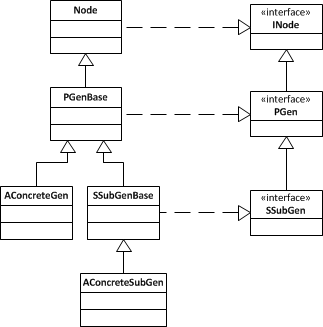
\includegraphics[width=\textwidth]
        {Images/asthierch.png}}
        \caption{\label{fig:AST General Architecture} The AST's General Architecture \parencite{vdmwikiast}}
      \end{figure}.

Nodes have fields which hold information on their values, as well as fields which hold information about, and provide access to, their children and ancestors. Neighbouring nodes - children and ancestor nodes - can be used to infer the structure of the AST surrounding any given node. Child nodes are fields of their parent nodes, this provides the tree structure of the AST. The highest-level class entity in the AST is the abstract \lstinline[language=Java]{Node} class which implements, and provides default definitions for, methods in the \lstinline[language=Java]{INode} interface. This interface defines common behaviour of all nodes in the AST whether they are binary expressions or function patterns. To name but a few, the INode interface contains abstract methods like \lstinline[language=Java]{parent()}, \lstinline[language=Java]{getChildren()} and \lstinline[language=Java]{removeChild()} which all allow for the AST to be manipulated accordingly by visitor classes later. The INode interface also includes abstract \lstinline[language=Java]{apply()} methods to support the visitor pattern for various adaptors, these concepts are explained in detail in section \ref{vp}. The \lstinline[language=Java]{PGen} interface is implemented by \lstinline[language=Java]{PGenBase} which extends \lstinline[language=Java]{Node} and is extended by \lstinline[language=Java]{SSubGenBase} which implements the \lstinline[language=Java]{SSubGen} interface. Evidently then, the structure of the AST is intricate but does provide excellent extensibility for tools such as the one that this project will attempt to implement.

A more concrete example of the AST's structure is the \lstinline[language=Java]{PExp} expressions family of VDM nodes seen in Fig\ref{fig:The AST hierarchy for a binary expression}. This example shows the AST hierarchy for a simple numeric binary expression like $a + b$. The concrete classes \lstinline[language=Java]{APlusNumericBinaryExp} and \lstinline[language=Java]{ATimesNumericBinaryExpIR} are leaf nodes as \lstinline[language=Java]{AConcreteSubGen} was in Fig\ref{fig:AST General Architecture}\begin{figure}
        \center{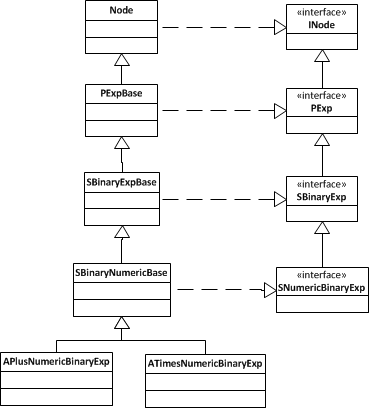
\includegraphics[width=\textwidth]
        {Images/vdmwikibinh.png}}
        \caption{\label{fig:The AST hierarchy for a binary expression} The AST hierarchy for a binary expression, in this case plus and times. \parencite{vdmwikiast}}
      \end{figure}

VDM is made up of a number of core modules, seen in Fig\ref{fig:VDM Modules Architecture}, which all work to build and manipulate the AST. It is worth mentioning that these modules are implemented in Overture, the Eclipse based IDE and VDM-SL platform. This project branches from the Overture GitHub, namely the cth/isagen branch maintained by Casper Thule Hansen,\parencite{VDM2ISAGit} and the entire development is an extension of the Overture package's \ttfamily\hl{CodeGen} module.\rmfamily\begin{figure}
        \center{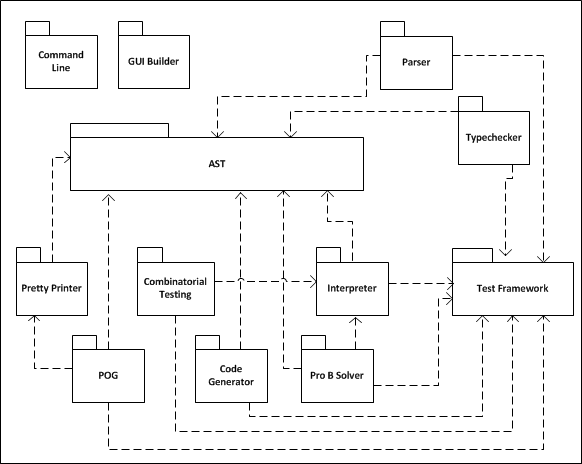
\includegraphics[width=\textwidth]
        {Images/vdmmodules.png}}
        \caption{\label{fig:VDM Modules Architecture} The Architecture of Core VDM Modules \parencite{OvertureWikiArchitectureDescription}}
      \end{figure}.
Fundamentally, all modules are built around the Abstract Syntax Tree (AST), all modules are written in pure Java. A very brief overview of the most important modules is as follows: \begin{itemize}
	\item The \ttfamily\hl{Parser} \rmfamily reads a VDM model and constructs its AST.
	\item After the operation of the \ttfamily\hl{Parser} \rmfamily, an AST is built. The \ttfamily\hl{Typechecker} \rmfamily module validates this AST and assigns types to each node, one such check might test if a given union type contains a Boolean type. An output of this stage is an Intermediate Representation, see \ref{cgair}.
	\item The \ttfamily\hl{Interpreter} \rmfamily module is responsible for executing the AST constructed from VDM Models by the \ttfamily\hl{Parser} \rmfamily, and interacting with the user.
	\end{itemize}


The main module of interest to this project in particular however; is the \ttfamily\hl{Code Generator} \rmfamily, in which lies the base \ttfamily\hl{Code Generator} \rmfamily that generates an Intermediate Representation (IR), and the \lstinline[language=Java]{IsaGen} package which manipulates that IR and contains all of the code written for the entirety of this project.

\subsection{Code Generator \& Intermediate Representation} \label{cgair}
After the \ttfamily\hl{Parser} \rmfamily, \ttfamily\hl{Typechecker} \rmfamily and their subsequent modules have completed operation \footnote{But before any output is produced by the \ttfamily\hl{Interpreter} \rmfamily or its subsequent modules.}, an Intermediate Representation (IR) is output. An IR is commonly used in programming languages to provide extensibility for Code Generators such as the Isabelle/HOL generator in question. An IR is a representation of a program between the source and target programming languages; after VDM has been compiled into an AST but before it is translated into Java or C++, or HOL here. The IR is independent of its source or target languages and is meant to provide a common ground, an interface of sorts between different tools and languages operating on one AST, similar is the way that Latin is used in the classification of wildlife, \lstinline[language=Java]{AAndBoolBinaryExpIR} IR node is an \lstinline[language=Java]{AAndBoolBinaryExpIR} node in both VDM and Isabelle ASTs. The IR allows the translation tool to analyse and manipulate an AST without repeatedly translating to and from VDM and Isabelle and allows the tool to have a pre-type-checked AST to work with. This is beneficial as we do not need to type check again in Isabelle after translation, the translation is broken up into manageable parts. A type-checked binary expression in IR is still a validated and type checked binary expression in Isabelle, or else it would not have been parsed to the IR AST by the \ttfamily\hl{Parser} \rmfamily and \ttfamily\hl{Typechecker} \rmfamily.

The \ttfamily\hl{Code Generator} \rmfamily module contains a base \ttfamily\hl{Code Generator} \rmfamily class which is responsible for providing access to the IR. Sub classing this class gives access to the IR and some valuable AST settings information. This Isabelle/HOL translator, which works within the \ttfamily\hl{Code Generator} \rmfamily module, approximately follows a five-step methodology originally proposed in the 13th Overture Workshop\parencite{overtureproceedings} and reads like so: [1] set-up, [2] add new nodes, [3] transform the IR, [4] generate syntax, [5] validate the translation.  

\begin{figure}
        \center{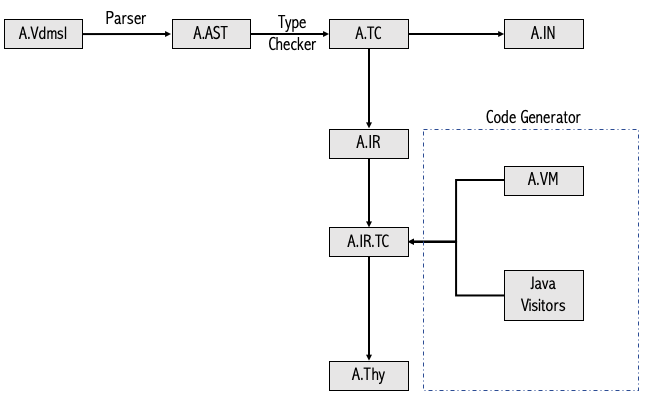
\includegraphics[width=\textwidth]
        {Images/FileOuts.png}}
        \caption{\label{fig:OES} The output progression of the A.vdmsl file.}
\end{figure}

\section{Methodology}
This section will describe the established methodology closely followed by this project as well as explanations of tools and technologies involved in its implementation.

	\subsection{	[1] Set-up a CGP extension} \label{s1}
	Have a class which extends the \lstinline[language=Java]{CodeGenBase} class and create a new template manager which will provide access to the template structure class provided by the \ttfamily\hl{Code Generator} \rmfamily module. Lastly, set up a basic testing facility, Overture, the Eclipse based IDE and VDM-SL interpreter utility in which we write VDM-SL, provides a test framework, this should be used to set up the tests. 
	\subsection{	[2] Add New Nodes}
	If the target language is significantly different from the first, then new nodes may need to be created and added to the AST. In the case of Isabelle, new nodes were needed quite often. In fact, almost every operation required addition of new Expression, Definition or Pattern nodes to the IR AST. This is because, as mentioned previously, an Isabelle translation requires explicit translation of every construct, for example invariants, pre and post conditions are translated as separate functions - contrary to how VDM handles say, functions, with pre and post conditions attached to the definition as VDM AST node fields.
	\subsection{	[3] Transform the IR} \label{ttir}
	This step transforms the AST so that the target language can be generated from it in the next stage. Constructs that are not supported in the target language are transformed away and fields and nodes are adjusted, or constructs removed altogether. There are two types of transformation applied to the AST: 
   	\begin{itemize}
	   \item A partial transformation. A partial transformation is trivial to apply but is limited in the way that it can only change the internal structure of the node - like fields, method overrides and so on. A partial transformation does not make large changes to the AST and so does not interfere greatly with its structure. Rarely, only minor adjustments need be made to an ancestor or a child of a partially transformed construct and this is often easily or even automatically achieved with implemented get and set methods.
	   \item A total transformation. Total transformations can change the node itself; the node can be transformed into a different node through type casts for example, removed and replaced with a different node or removed from the tree entirely. Total transformations are difficult to perform and, as I discovered during my implementation of the tool, volatile and vulnerable to anomalous behaviour, sub nodes of the node must on occasion be subsequently changed significantly according to the changes made to their ancestor. The following code snippet from the overture git shows how to apply transformations.
	   \begin{lstlisting}
	   	List<ExtIrClassDeclStatus> transformed = new Vector<>();

		for (IRClassDeclStatus status : untransformed)
		{
		  // Partial transformation applied directly
		  PartialTransformationFoo t1 = new PartialTransformationFoo();
		  generator.applyPartialTransformation(status, t1);

		  // Total transformations need wrapping
		  ExtIrClassDeclStatus eStatus = new ExtIrClassDeclStatus(status);
		  TotalTransformationBar t2 = new TotalTransformationBar();
		  generator.applyTotalTransformation(eStatus, t2);
		  transformed.add(eStatus);
		}
	  	\end{lstlisting}\parencite{vdmwikicgp}
 	\end{itemize}
	Total transformations need extra work within the \lstinline[language=Java]{TotalTransformationBar} to harmonize the tree with the change to its nodes. Transformations themselves take the form of visitor classes, the \lstinline[language=Java]{PartialTransformationFoo} class above is a visitor class. The visitor pattern is important and so it is given its own section in \ref{vp}.

	\subsubsection{The Visitor Pattern} \label{vp}
	Manipulating the VDM AST directly is highly discouraged, the system of modules and their dependencies is far too complex to handle direct changes to its central component. The idea of a visitor design pattern is to detach an algorithm from the data that it operates on, in this case to detach the VDM AST from code generation transformations performing potentially erroneous meddling. As mentioned in section \ref{ead}, the \lstinline[language=Java]{INode} interface that is the highest level of abstraction in the VDM AST enforces \lstinline[language=Java]{apply()} methods. All Nodes in the AST have \lstinline[language=Java]{apply()} methods as they enable the visitor pattern. Where before, something like \lstinline[language=Java]{node.changeParent()}, becomes instead \lstinline[language=Java]{node.apply(parentChangeVisitor)} where \lstinline[language=Java]{parentChangeVisitor} is a Java class with methods that change the parent of a node. Almost every time that we interact with the AST this pattern is used. The \lstinline[language=Java]{apply()} method, implemented by each node, allows each node of the AST to control the way in which it is individually transformed according to its own subtle intricacies that would not be, nor should have to be, strictly adhered to by external classes. The \lstinline[language=Java]{apply()} method, and by extension the visitor pattern, hence gives control of any interaction with the AST, over to the AST nodes' classes, each of which know precisely how to handle interaction safely in their own unique way, because of this, the AST is never damaged or malformed. 

	The AST classes will only accept a class in their \lstinline[language=Java]{apply()} functions if that class is a visitor. A class is identified as a visitor by extending, sub-classing, an adaptor class in the \lstinline[language=Java]{org.overture.ast.analysis} package, an adaptor class \textbf{adapts} AST interaction by visitors into a safe one. More on the various analysis adaptor classes in this package is discussed later in this section. In order for a visitor to be able to interact with different types and families of nodes, they must be equipped with a method containing functionality for the \emph{case} that certain nodes might be encountered.

	Cases are a powerful construct within the visitor pattern, they allow the programmer to do away with exceedingly long control blocks used to test for the presence of specific nodes, any large code blocks can be stored in a separate visitor class containing case methods for what to do for each different node family or type. Each class in the \lstinline[language=Java]{org.overture.ast.analysis} package is filled with case methods for every type of node. The \lstinline[language=Java]{DepthFirstAnalysisAdaptor} class contains approximately $16,000$ lines of code the majority of which are empty or basic case methods which are overridable so that the sub-classed visitor can add its own functionality for that node case. Each method takes as a parameter, a node of the type that it is the case for. To name but a minute few in this class:
	\begin{lstlisting}[language=Java]
	caseARealPatternIR(ARealPatternIR)
	caseARecordDeclIR(ARecordDeclIR)
	caseARecordModExpIR(ARecordModExpIR)
	caseARecordModifierIR(ARecordModifierIR)
	caseARecordPatternIR(ARecordPatternIR)
	caseARecordTypeIR(ARecordTypeIR)
	caseARemNumericBinaryExpIR(ARemNumericBinaryExpIR)
	caseARenamedDeclIR(ARenamedDeclIR)
	caseARepeatTraceDeclIR(ARepeatTraceDeclIR)
	caseAReturnStmIR(AReturnStmIR)
	caseAReverseUnaryExpIR(AReverseUnaryExpIR)
	caseASameBaseClassExpIR(ASameBaseClassExpIR)
	caseASameClassExpIR(ASameClassExpIR)
	\end{lstlisting}
	If, for example, the programmer would like to create a visitor that counts the number of fields in \lstinline[language=Java]{ARecordDeclIR}\footnote{The IR node for a declaration of a record type.} then they would write a class like so:
	\begin{lstlisting}[language=Java]
	public class EmptySeqVisitor extends AnalysisAdaptor {

	  int nodeCount;
	  
	  @Override
	  public void caseARecordDeclIR(ARecordDeclIR node)
	      throws AnalysisException {
	  
	    nodeCount = node.getFields().size();
	    //_fields is a NodeList<AFieldDeclIR>() field in ARecordDeclIR. NodeList is a VDM class in the AST package implementing list functionality.
	    
	  }
	  
	}
	\end{lstlisting}

	The \lstinline[language=Java]{org.overture.ast.analysis} package contains additional classes, adaptors, to \lstinline[language=Java]{AnalysisAdaptor} which can be extended to provide various AST interactions, parameter passing, return values, or both. 
	\begin{enumerate}
		\item \lstinline[language=Java]{AnalysisAdaptor} The easiest way to create a visitor to the AST, it takes no parameters and the return type of its overridden methods are always void. Such a visitor can be used, for example, to count occurrences of a type of node by incrementing a field as the visitor encounters a node of a certain type. 
		\item \lstinline[language=Java]{QuestionAdaptor<Q>} Allows the visitor to pass information to the AnalysisAdaptor as a generic type parameter, though this parameter must be the same for all cases in a given visitor. In a question visitor the parameter object \lstinline[language=Java]{<Q>} is passed as a second parameter to every method in the visitor. It can be used to check the equality of a node or its fields, to set a parameter of a node to a different value and so on.
		\item \lstinline[language=Java]{AnswerAdaptor<A>} Allows the visitor to define a return type and gather data from the AST so long as the data is of type \lstinline[language=Java]{<A>}. Every method in the visitor has a return type of \lstinline[language=Java]{<A>}. Extending this class requires the visitor to implement two additional methods \lstinline[language=Java]{createNewReturnValue(INode node)} and \lstinline[language=Java]{createNewReturnValue(Object node)}, as something must be returned, these methods are invoked when no other case is matched.
		\item \lstinline[language=Java]{QuestionAnswerAdaptor<Q,A>} As may be evident from the name, a visitor that is a subclass of this class can both pass parameters of type \lstinline[language=Java]{<Q>} and take a return type of \lstinline[language=Java]{<A>}. This class allows for the most flexibility of the three and must implement the same methods as the proceeding classes in this list.
		\item \lstinline[language=Java]{DepthFirstAnalysisAdaptor} This is used frequently in this project; this adaptor allows a visitor to perform a depth first tree traversal of the AST and perform analysis as it does so. A visitor that is a subclass of this class is given the same methods to implement and override as the \lstinline[language=Java]{AnalysisAdaptor} class with the addition of \lstinline[language=Java]{public void setVisitedNodes(Set<INode> value)} and the field \lstinline[language=Java]{_visitedNodes} which allow sub-classed visitors to access the nodes visited during the depth first tree traversal. This is a particularly useful class for modifying the AST, nodes that need to be worked on can be on wildly different sub-trees due to the differences between Isabelle and VDM.
		\item \lstinline[language=Java]{DepthFirstAnalysisAdaptorAnswer<A>} Performs a depth first analysis of the tree with the addition of answer functionality described in  \lstinline[language=Java]{AnswerAdaptor<A>} above.
		\item \lstinline[language=Java]{DepthFirstAnalysisAdaptorQuestion<Q>} Performs a depth first analysis of the tree with the addition of question functionality described in  \lstinline[language=Java]{QuestionAdaptor<A>} above.
		\item \lstinline[language=Java]{DepthFirstAnalysisAdaptorQuestionAnswer<Q,A>} Performs a depth first analysis of the tree with the addition of question/answer functionality described in  \lstinline[language=Java]{QuestionAnswerAdaptor<A>} above.
	\end{enumerate} 


	\subsection{	[4] Generate Target Language Syntax}
	Now that the AST has been transformed into a state ready to be translated into an AST of its target language, it is passed into the syntax generation framework of the \ttfamily\hl{Code Generator} \rmfamily module. At this stage the \ttfamily\hl{Code Generator} \rmfamily module traverses the IR AST and creates translated target language code as a String for each node. The \ttfamily\hl{Code Generator} \rmfamily detects the node's type and then creates code for it by populating pre-defined Apache Velocity templates, see \ref{av} for a description of Apache Velocity and its application to this project.
	\subsubsection{Apache Velocity} \label{av}
	Apache Velocity is a Java based template engine in which a \ttfamily\hl{.vm} \rmfamily file is written containing Velocity syntax, the velocity syntax accesses variables defined in Java code and allows the programmer to interweave their values with appropriate syntax, lexicon and document structure to create the desired output string or file. Some example Velocity syntax is:
	\hfill\break
	\begin{lstlisting}[language=Velocity]
		($Isa.trans($node.Left) \<and> $Isa.trans($node.Right))
	\end{lstlisting} 
	\hfill\break
	This creates essentially place holders for the result of Java computations that will create a value for a Java translation method \lstinline[language=Java]{trans(INode node)} which will have passed into it the node which is the left hand side value of the binary \ttfamily\hl{and} \rmfamily expression followed by the Isabelle/HOL symbol for \ttfamily\hl{and} \rmfamily \lstinline[language=Isabelle, mathescape]{\<and>}\footnote{which will be translated into the HOL symbol $\wedge$} followed by the node which is the right hand side of the \ttfamily\hl{and} \rmfamily expression - we will get something like $A \wedge B$ in Isabelle. The and template is a trivial example but templates as complex as entire function definition structures can be achieved.  
	\hfill\break
	\hfill\break
	\hfill\break
	\hfill\break
	\textbf{Velocity}
	\begin{lstlisting}[language=Velocity, caption=The Velocity template for function declarations. Below is a translation showing how one such template is used in practice.]
	#macro ( transIdentifiers $node )
	#foreach($p in $node.FormalParams)
	$Isa.trans($p.pattern)##
	#end
	#end

	definition
	#if ("$Isa.transTypeParams($node.MethodType.Params)" == "")
		$node.Name :: "$Isa.trans($node.MethodType.Result)"
	#else
		$node.Name :: "$Isa.transTypeParams($node.MethodType.Params) \<Rightarrow> $Isa.trans($node.MethodType.Result)"
	#end
	    where
	    "$node.Name #transIdentifiers($node) \<equiv> $Isa.trans($node.Body)"
	\end{lstlisting} 

	\textbf{Translation}
	\hfill\break
	\hfill\break
	\pagecolor{bgcolor}
	\ttfamily
	\syntaxNULL{}\gutter{\ \ \ \ 1{|}\ }\syntaxKEYWORDA{theory}{\ }A\hspace*{\fill}\\
	\gutter{\ \ \ \ 2{|}\ }{\ }{\ }{\ }{\ }{\ }{\ }\syntaxKEYWORDB{imports}{\ }VDMToolkit\hspace*{\fill}\\
	\gutter{\ \ \ \ 3{|}\ }{\ }{\ }{\ }{\ }\syntaxKEYWORDB{begin}\hspace*{\fill}\\
	\gutter{\ \ \ \ 4{|}\ }\hspace*{\fill}\\
	\gutterH{\ \ \ \ 5{|}\ }\hspace*{\fill}\\
	\gutter{\ \ \ \ 6{|}\ }{\ }{\ }{\ }{\ }\syntaxKEYWORDA{definition}\hspace*{\fill}\\
	\gutter{\ \ \ \ 7{|}\ }{\ }{\ }{\ }{\ }{\ }{\ }f{\ }\syntaxOPERATOR{::}{\ }\syntaxLITERALA{"VDMNat}\hspace*{\fill}\\
	\gutter{\ \ \ \ 8{|}\ }\syntaxLITERALA{{\ }{\ }}\syntaxLITERALA{{\ }{\ }}\syntaxLITERALA{{\ }}\syntaxLITERALA{\usebox{\backslashbox}}\syntaxLITERALA{\usebox{\lessthan}}\syntaxLITERALA{R}\syntaxLITERALA{i}\syntaxLITERALA{g}\syntaxLITERALA{h}\syntaxLITERALA{t}\syntaxLITERALA{a}\syntaxLITERALA{r}\syntaxLITERALA{r}\syntaxLITERALA{o}\syntaxLITERALA{w}\syntaxLITERALA{\usebox{\greaterthan}}\syntaxLITERALA{{\ }}\syntaxLITERALA{V}\syntaxLITERALA{D}\syntaxLITERALA{M}\syntaxLITERALA{N}\syntaxLITERALA{a}\syntaxLITERALA{t}\hspace*{\fill}\\
	\gutter{\ \ \ \ 9{|}\ }\syntaxLITERALA{{\ }{\ }}\syntaxLITERALA{{\ }{\ }}\syntaxLITERALA{{\ }}\syntaxLITERALA{\usebox{\backslashbox}}\syntaxLITERALA{\usebox{\lessthan}}\syntaxLITERALA{R}\syntaxLITERALA{i}\syntaxLITERALA{g}\syntaxLITERALA{h}\syntaxLITERALA{t}\syntaxLITERALA{a}\syntaxLITERALA{r}\syntaxLITERALA{r}\syntaxLITERALA{o}\syntaxLITERALA{w}\syntaxLITERALA{\usebox{\greaterthan}}\syntaxLITERALA{{\ }}\syntaxLITERALA{V}\syntaxLITERALA{D}\syntaxLITERALA{M}\syntaxLITERALA{N}\syntaxLITERALA{a}\syntaxLITERALA{t}\hspace*{\fill}\\
	\gutterH{\ \ \ 10{|}\ }\syntaxLITERALA{{\ }{\ }}\syntaxLITERALA{{\ }{\ }}\syntaxLITERALA{"}\hspace*{\fill}\\
	\gutter{\ \ \ 11{|}\ }{\ }{\ }{\ }{\ }{\ }{\ }{\ }{\ }\syntaxKEYWORDB{where}\hspace*{\fill}\\
	\gutter{\ \ \ 12{|}\ }{\ }{\ }{\ }{\ }{\ }{\ }{\ }{\ }\syntaxLITERALA{"f{\ }x{\ }y{\ }{\ }\usebox{\backslashbox}\usebox{\lessthan}equiv\usebox{\greaterthan}{\ }x"}\hspace*{\fill}\\
	\gutter{\ \ \ 13{|}\ }\hspace*{\fill}\\
	\gutter{\ \ \ 14{|}\ }\hspace*{\fill}\\
	\gutterH{\ \ \ 15{|}\ }{\ }{\ }{\ }{\ }\syntaxKEYWORDA{definition}\hspace*{\fill}\\
	\gutter{\ \ \ 16{|}\ }{\ }{\ }{\ }{\ }{\ }{\ }pre\usebox{\underscorebox}f{\ }\syntaxOPERATOR{::}{\ }\syntaxLITERALA{"VDMNat}\hspace*{\fill}\\
	\gutter{\ \ \ 17{|}\ }\syntaxLITERALA{{\ }{\ }}\syntaxLITERALA{{\ }{\ }}\syntaxLITERALA{{\ }}\syntaxLITERALA{\usebox{\backslashbox}}\syntaxLITERALA{\usebox{\lessthan}}\syntaxLITERALA{R}\syntaxLITERALA{i}\syntaxLITERALA{g}\syntaxLITERALA{h}\syntaxLITERALA{t}\syntaxLITERALA{a}\syntaxLITERALA{r}\syntaxLITERALA{r}\syntaxLITERALA{o}\syntaxLITERALA{w}\syntaxLITERALA{\usebox{\greaterthan}}\syntaxLITERALA{{\ }}\syntaxLITERALA{V}\syntaxLITERALA{D}\syntaxLITERALA{M}\syntaxLITERALA{N}\syntaxLITERALA{a}\syntaxLITERALA{t}\hspace*{\fill}\\
	\gutter{\ \ \ 18{|}\ }\syntaxLITERALA{{\ }{\ }}\syntaxLITERALA{{\ }{\ }}\syntaxLITERALA{{\ }}\syntaxLITERALA{\usebox{\backslashbox}}\syntaxLITERALA{\usebox{\lessthan}}\syntaxLITERALA{R}\syntaxLITERALA{i}\syntaxLITERALA{g}\syntaxLITERALA{h}\syntaxLITERALA{t}\syntaxLITERALA{a}\syntaxLITERALA{r}\syntaxLITERALA{r}\syntaxLITERALA{o}\syntaxLITERALA{w}\syntaxLITERALA{\usebox{\greaterthan}}\syntaxLITERALA{{\ }}\syntaxLITERALA{\usebox{\backslashbox}}\syntaxLITERALA{\usebox{\lessthan}}\syntaxLITERALA{b}\syntaxLITERALA{o}\syntaxLITERALA{o}\syntaxLITERALA{l}\syntaxLITERALA{\usebox{\greaterthan}}\syntaxLITERALA{"}\hspace*{\fill}\\
	\gutter{\ \ \ 19{|}\ }{\ }{\ }{\ }{\ }{\ }{\ }{\ }{\ }\syntaxKEYWORDB{where}\hspace*{\fill}\\
	\gutterH{\ \ \ 20{|}\ }{\ }{\ }{\ }{\ }{\ }{\ }{\ }{\ }\syntaxLITERALA{"pre\usebox{\underscorebox}f{\ }x{\ }y{\ }{\ }\usebox{\backslashbox}\usebox{\lessthan}equiv\usebox{\greaterthan}{\ }(isa\usebox{\underscorebox}invVDMNat{\ }x{\ }\usebox{\backslashbox}\usebox{\lessthan}and\usebox{\greaterthan}{\ }isa\usebox{\underscorebox}invVDMNat{\ }y)"}\hspace*{\fill}\\
	\gutter{\ \ \ 21{|}\ }\hspace*{\fill}\\
	\gutter{\ \ \ 22{|}\ }\hspace*{\fill}\\
	\gutter{\ \ \ 23{|}\ }{\ }{\ }{\ }{\ }\syntaxKEYWORDA{definition}\hspace*{\fill}\\
	\gutter{\ \ \ 24{|}\ }{\ }{\ }{\ }{\ }{\ }{\ }post\usebox{\underscorebox}f{\ }\syntaxOPERATOR{::}{\ }\syntaxLITERALA{"VDMNat}\hspace*{\fill}\\
	\gutterH{\ \ \ 25{|}\ }\syntaxLITERALA{{\ }{\ }}\syntaxLITERALA{{\ }{\ }}\syntaxLITERALA{{\ }}\syntaxLITERALA{\usebox{\backslashbox}}\syntaxLITERALA{\usebox{\lessthan}}\syntaxLITERALA{R}\syntaxLITERALA{i}\syntaxLITERALA{g}\syntaxLITERALA{h}\syntaxLITERALA{t}\syntaxLITERALA{a}\syntaxLITERALA{r}\syntaxLITERALA{r}\syntaxLITERALA{o}\syntaxLITERALA{w}\syntaxLITERALA{\usebox{\greaterthan}}\syntaxLITERALA{{\ }}\syntaxLITERALA{V}\syntaxLITERALA{D}\syntaxLITERALA{M}\syntaxLITERALA{N}\syntaxLITERALA{a}\syntaxLITERALA{t}\hspace*{\fill}\\
	\gutter{\ \ \ 26{|}\ }\syntaxLITERALA{{\ }{\ }}\syntaxLITERALA{{\ }{\ }}\syntaxLITERALA{{\ }}\syntaxLITERALA{\usebox{\backslashbox}}\syntaxLITERALA{\usebox{\lessthan}}\syntaxLITERALA{R}\syntaxLITERALA{i}\syntaxLITERALA{g}\syntaxLITERALA{h}\syntaxLITERALA{t}\syntaxLITERALA{a}\syntaxLITERALA{r}\syntaxLITERALA{r}\syntaxLITERALA{o}\syntaxLITERALA{w}\syntaxLITERALA{\usebox{\greaterthan}}\syntaxLITERALA{{\ }}\syntaxLITERALA{V}\syntaxLITERALA{D}\syntaxLITERALA{M}\syntaxLITERALA{N}\syntaxLITERALA{a}\syntaxLITERALA{t}\hspace*{\fill}\\
	\gutter{\ \ \ 27{|}\ }\syntaxLITERALA{{\ }{\ }}\syntaxLITERALA{{\ }{\ }}\syntaxLITERALA{{\ }}\syntaxLITERALA{\usebox{\backslashbox}}\syntaxLITERALA{\usebox{\lessthan}}\syntaxLITERALA{R}\syntaxLITERALA{i}\syntaxLITERALA{g}\syntaxLITERALA{h}\syntaxLITERALA{t}\syntaxLITERALA{a}\syntaxLITERALA{r}\syntaxLITERALA{r}\syntaxLITERALA{o}\syntaxLITERALA{w}\syntaxLITERALA{\usebox{\greaterthan}}\syntaxLITERALA{{\ }}\syntaxLITERALA{\usebox{\backslashbox}}\syntaxLITERALA{\usebox{\lessthan}}\syntaxLITERALA{b}\syntaxLITERALA{o}\syntaxLITERALA{o}\syntaxLITERALA{l}\syntaxLITERALA{\usebox{\greaterthan}}\syntaxLITERALA{"}\hspace*{\fill}\\
	\gutter{\ \ \ 28{|}\ }{\ }{\ }{\ }{\ }{\ }{\ }{\ }{\ }\syntaxKEYWORDB{where}\hspace*{\fill}\\
	\gutter{\ \ \ 29{|}\ }{\ }{\ }{\ }{\ }{\ }{\ }{\ }{\ }\syntaxLITERALA{"post\usebox{\underscorebox}f{\ }x{\ }y{\ }RESULT{\ }{\ }\usebox{\backslashbox}\usebox{\lessthan}equiv\usebox{\greaterthan}{\ }(isa\usebox{\underscorebox}invVDMNat{\ }x{\ }\usebox{\backslashbox}\usebox{\lessthan}and\usebox{\greaterthan}{\ }\hspace*{\fill}(isa\usebox{\underscorebox}invVDMNat{\ }\hspace*{\fill}y{\ }\usebox{\backslashbox}\usebox{\lessthan}and\usebox{\greaterthan}{\ }isa\usebox{\underscorebox}invVDMNat{\ }RESULT))"}\hspace*{\fill}\\
	\gutterH{\ \ \ 30{|}\ }\hspace*{\fill}\\
	\gutter{\ \ \ 31{|}\ }{\ }{\ }{\ }{\ }\syntaxKEYWORDB{end}\hspace*{\fill}\\
	\mbox{}
	\hfill\break
	\rmfamily
	By this mechanism, the \ttfamily\ttfamily\hl{Code Generator} \rmfamily \rmfamily module traverses the AST and populates the templates while the subsequent steps transform the nodes in the AST by computing and manipulating them in order to provide Velocity with the correct variable values. The purpose of the subsequent steps are to prevent the programmer from having to write large velocity files, a well organised visitor pattern and translator should make their target velocity templates as short as possible, one praise of this project is that the velocity files never exceed any more than $19$ lines of code and are approximately $2.67$, rounded to $3$, lines long on average, this includes white-space. Fig\ref{fig:toolStructure} shows an in detail diagram of these steps' outputs.

	\subsection{	[5] Validate} \label{vdt}
	The validation step involves comparison of the output with a known correct result file. Result files are kept very simple and each construct is separate, for example we have one file to test \lstinline[language=Java]{AIntNumericBasicTypeIR} node translation and it is kept as simple as possible. All test files have the \lstinline[language=Java]{.vdmsl} file extension and have one corresponding \lstinline[language=Java]{.vdmsl.result} file which contains the expected translation of a construct. For example, the file \lstinline[language=Java]{Int.vdmsl} has a corresponding result file \lstinline[language=Java]{Int.vdmsl.result}. 
	\begin{vdmsl}[label=lst:Int.vdmsl,caption=Int.vdmsl]
	types
	XType = int;
	\end{vdmsl}
	\begin{vdmsl}[label=lst:Int.vdmsl.result, caption=Int.vdmsl.result]
	{"translation":"theory DEFAULT
	imports VDMToolkit
	begin

	type_synonym XType \= \"VDMInt\"




	definition
	    inv_XType :: \"(XType) \\<Rightarrow> \\<bool> \"
	    where
	    \"inv_XType x \\<equiv> isa_invTrue x\"

	end","errors":false}
	\end{vdmsl}  
	A test passes if the output of the first file, after running through all of the core modules and the translation tool, matches the second.

	\section{Previous Tool Implementation Work}
	\subsection{Previously Completed Step [1] Set-up A CGP Extension}

	Before starting this project, Casper Thule Hansen, PhD Researcher of Aarhus University Denmark\parencite{casper}, had completed the important and tricky first step of the methodology described in \ref{s1}.\parencite{VDM2ISAGit}
	\begin{figure}
        \center{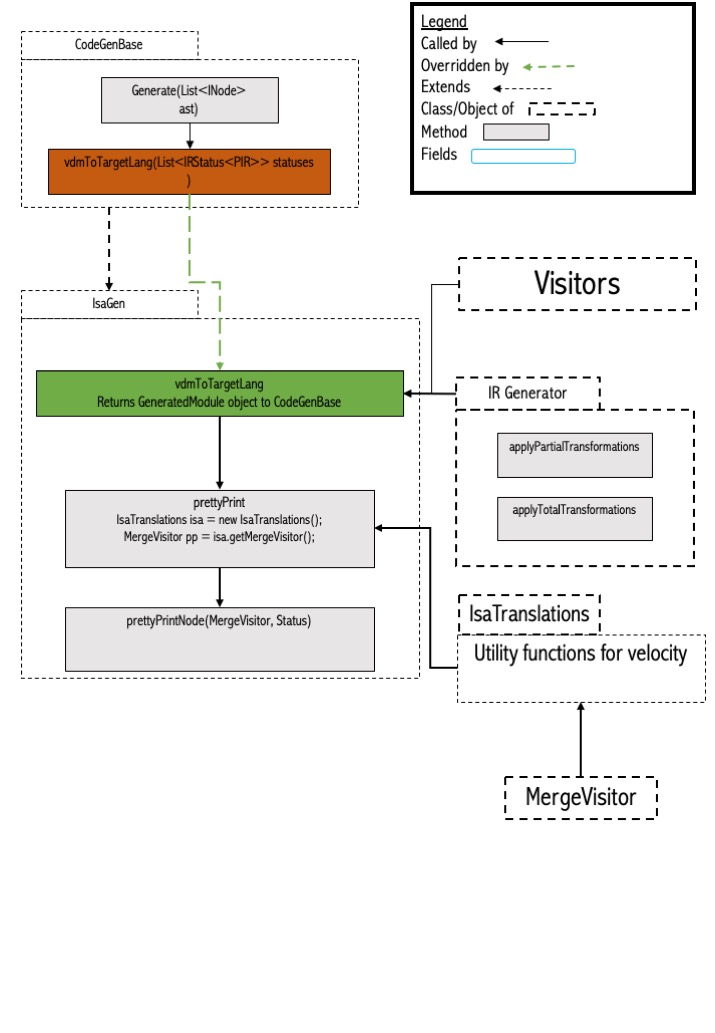
\includegraphics[width=\textwidth]
        {Images/toolStructure.jpg}}
        \caption{\label{fig:toolStructure} The tools structure at the set up stage. \parencite{vdmwikiast}}
     \end{figure}.
    As mentioned in \ref{s1} this is the first step in creating a CGP (Code Generation Platform) extension.\ref{fig:toolStructure} \lstinline[language=Java]{IsaGen}, extends the \lstinline[language=Java]{CodeGenBase} class and the \lstinline[language=Java]{IsaTranslations} class serves as a template manager, this class provides access to the template structure provided by the \ttfamily\hl{Code Generator} \rmfamily module by creating a \lstinline[language=Java]{MergeVisitor} object as a field as well as a list of callable templates, \lstinline[language=Java]{TemplateCallable[] templateCallables} from the \lstinline[language=Java]{org.overture.codegen.merging.TemplateCallable} package in the CGP module, for accessing the various Velocity templates for each node.

    The \lstinline[language=Java]{IsaGen} class overrides the \lstinline[language=Java]{genVDMToTargetLang} method\footnote{See appendix \ref{beforecode}, section \ref{IsaGenbefore}to see \lstinline[language=Java]{genVdmToTargetLang} before development, and appendix \ref{aftercode}, section \ref{IsaGenafter}, for after development} in \lstinline[language=Java]{CodeGenBase}. This method is used by \lstinline[language=Java]{CodeGenBase} and the CGP to generate the target language data. By overriding it, it becomes our main point of interaction with the CGP and so this is where we perform our transformations. We do so by placing visitor classes in this method, taking \lstinline[language=Java]{status} as an argument. 

    Once this method has initialised the fields of a \lstinline[language=Java]{GeneratedModule} object, it is returned to the calling method in \lstinline[language=Java]{CodeGenBase}, \lstinline[language=Java]{generate()}, which is used by \lstinline[language=Java]{CodeGenBase} in a series of steps by the CGP to create the target language output.
   
	The \lstinline[language=Java]{getInfo()} method provides access to AST settings while the parameter \lstinline[language=Java]{List<IRStatus<PIR>> statuses} provides access to the AST itself. The method generates the IR using the CGP and Typechecker module through several calls to CGP methods during the lambda function at the top of the method. 

	As the final step in stage one, a test framework had also been set up. The test that I used was the JUnit class \lstinline[language=Java]{IsaGenParamTest}. The test strategy was that all tests should pass and before this project one already did, integer, as described later in this section\footnote{The full class can be seen in appendix \ref{testing}}. It is necessary to understand that this test class was set up as an array of skipped tests, the strategy was to activate a test, make it pass and then continue to the next.\footnote{See appendix \ref{testing} for the full code.}

	
	\subsection{Previous Work on Step [2] Add New Nodes \& Step [3] Transform The IR} \label{pwos}

	Some parts of the transformation step described in \ref{ttir}, were also implemented prior to this project.	As the tool goes over the AST it applies visitor classes to its nodes. Total transformations are applied to each status, by the  \lstinline[language=Java]{GroupMutRecs} visitor, recursion cycles in the AST's structure are transformed away before translation to Isabelle. The \lstinline[language=Java]{SortDependencies} visitor is applied to \lstinline[language=Java]{AModuleDeclIR} nodes, this sets up the theory file, dependencies, imports, name etc. . The \lstinline[language=Java]{AModuleDeclIR} node is the highest level element of the theory file, it is the file definition that encase all declarations within it, in Isabelle it is marked by the \lstinline[language=Isabelle, mathescape]{theory} keyword at the top of a \lstinline[language=Isabelle, mathescape]{.thy} file. In this visitor we have the case: 
	\begin{lstlisting}[language=Java]
	@Override
    public void caseAModuleDeclIR(AModuleDeclIR node) throws AnalysisException {
        result = new AModuleDeclIR();
        result.setExports(node.getExports());
        result.setImport(node.getImport());
        result.setIsDLModule(node.getIsDLModule());
        result.setIsFlat(node.getIsFlat());
        result.setMetaData(node.getMetaData());
        result.setName(node.getName());
        result.setSourceNode(node.getSourceNode());
        result.setTag(node.getTag());
        result.setDecls(node.getDecls());
        filterFunctions(node.getDecls());
        calcDependencies();

    }
    \end{lstlisting}
    This clarifies the above, the module declaration, i.e. the file declaration, is set up by setting the above fields. The \lstinline[language=Java]{_decls}, declaration, child is particularly important, it holds all declarations in the file as a list. Adding a declaration to the \lstinline[language=Java]{AModuleDeclIR} 's \lstinline[language=Java]{_decls} list field adds it to the AST, and so the file, this will be seen later as it is the mechanism used to add to the AST. In short, the \lstinline[language=Java]{AModuleDeclIR} ancestor of a node is retrieved, the \lstinline[language=Java]{_decls} field is accessed using a get method, then a declaration is added to it.

    With the module declaration set up, visitor classes are then free to be applied to the AST nodes. Previous work had set up one example of how to manipulate the AST to set up classes properly, 
    \begin{lstlisting}[language=Java]
    IsaBasicTypesConv invConv = new IsaBasicTypesConv(getInfo(), this.transAssistant, vdmToolkitModuleIR);
    generator.applyPartialTransformation(status, invConv);
    \end{lstlisting}
    The visitor class \lstinline[language=Java]{IsaBasicTypesConv} contains a case for \lstinline[language=Java]{caseAIntNumericBasicTypeIR} which translates VDMToolkit's VDMInt types.\footnote{See appendix \ref{beforecode}, section \ref{IsaBasicTypesConvbefore}} The constructor of this visitor has a pattern that is commonly repeated throughout the visitors in this project. A lambda function goes through all of the type declarations in the VDMToolkit and maps their name to their IR node. Example: 
	\begin{lstlisting}[language=Java]
	{isa_VDMNat=privateATypeDeclIRisa_VDMNatint,  
	isa_VDMInt=privateATypeDeclIRisa_VDMIntint, 
	isa_VDMNat1=privateATypeDeclIRisa_VDMNat1int}
	\end{lstlisting}

	A description of the functionality provided by these classes will be present in section \ref{wd}, as this document explains changes made by the development process, so will it describe, by proxy, the similar mechanisms previously implemented here.\footnote{Appendix \ref{beforecode}, shows all of this code and classes at the start of the project.}

	\subsubsection{Invariant Generation} \label{iigt}
	Before development, the \lstinline[language=Java]{IsaInvGenTrans} invariant transformation visitor had been established. This visitor generates nodes that will contribute to building the invariant function declaration for a type.\footnote{See appendix \ref{beforecode}, section \ref{IsaInvGenTransbefore} for the before state of \lstinline[language=Java]{IsaInvGenTrans}} 
	This visitor grows significantly over the course of ensuing development as it is used to generate invariants differently per case, further case methods for field declarations\footnote{VDM value declarations} are added later. As with \lstinline[language=Java]{IsaBasicTypesConv}, a map for VDMToolkit types is initialised. Through an identical mechanism, this constructor has the addition of a map initialisation for VDMToolkit function types.
	\begin{lstlisting}[language=Java]
	this.isaFuncDeclIRMap = this.vdmToolkitModule.getDecls().stream().filter(d ->
	        {
	            if (d instanceof AFuncDeclIR)
	                return true;
	            else
	                return false;
	        }).map(d -> (AFuncDeclIR) d).collect(Collectors.toMap(x -> x.getName(), x -> x));
	\end{lstlisting}
	A lambda stream filters through all function declarations, of node type \lstinline[language=Java]{AFuncDeclIR}, in the VDMToolkit IR. These nodes correspond to invariant functions, and so this map is essentially an map of VDMToolkit invariant names to their declaration. 

	A case method for all type declarations was established that would generate invariants for a type declaration node.
	\begin{lstlisting}[language=Java]
	@Override
	    public void caseATypeDeclIR(ATypeDeclIR node) throws AnalysisException {
	\end{lstlisting}
	
	The state of this case method before development can be found in the appendices, appendix \ref{beforecode}, section \ref{IsaInvGenTransbefore}. Essentially, the method specified that if no invariant existed, a new function declaration node would be created along with a number of other nodes. These nodes would construct the fields of the function declaration before it is added to the AST, in the body of the generated invariant function, a check that \lstinline[language=Java]{isa_invTrue x} held of the type declaration. The details of these computations, and the resulting construction of invariant functions, are not detailed here as they are explained thoroughly in \ref{itag}.

	This method was limited in that it only generated invariants if none were there, where it could have concatenated existing invariants with additional generated necessary checks. At this stage the visitor only supported type declarations with this functionality.

	\section{Work Done in This Project}
	As step one was entirely set up by Casper Thule Hansen previously, the implementation of each construct starts at step [2] \ref{ttir} and goes through to step [5]\ref{vdt}. This section will not discuss every change made to achieve translation for each construct, but instead focus on implementation issues and headlines. This is because some additions or modifications are similar, and represent the same implementation issues and headlines. As such, the following section is structured like so: firstly, a more in depth overview of the development strategy; then, a test representing a VDM construct from \lstinline[language=Java]{IsaGenParamTest} will be activated, if there are relevant, and as yet uncovered programming issues and headlines they will be described, if not this construct test will be skipped.

	\subsection{Development Strategy}
	The goal of development was that all \lstinline[language=Java]{IsaGenParamTest} tests should pass, development only progressed when a test passed, in that sense \textbf{development was test driven}. I started with what should be the top of the VDM file, types, so that my approach was structured in a way that complimented the functional programming rules that defined my source and target languages. After, I moved on to values, then functions, then state. At each stage I repeated the five step methodology, previously discussed, in a cycle. I first transformed the IR to translate no more than what was already in the IR AST into Isabelle; next, I generated additional constructs, such as invariant function body expressions, to support the translation and then added them to the AST; I passed the resulting IR AST to the \lstinline[language=Java]{IsaGen} class and the \lstinline[language=Java]{applyPartialTransformations} method to generate the Isabelle syntax, at this stage I also added any necessary Velocity code, although this was rare; finally I validated the generated syntax with the relevant test.

	\subsection{No Invariant, Basic Numeric Type Translations}
	For basic numeric types, generating their translation was the same.\footnote{See appendix \ref{aftercode}, section \ref{IsaBasicTypesConvafter}.} All VDMToolkit types were simply added as cases to the \lstinline[language=Java]{IsaBasicTypesConv} class. The code within them was each time identical to the \lstinline[language=Java]{caseAIntNumericBasiTypeIR}, with the exception of their VDMToolkit name. To enable the function of these classes, I added string constants as fields of the class as with the \lstinline[language=Java]{private final static String isa_VDMInt = "isa_VDMInt";} field. 
	\subsubsection{Nat1 Example}
	\lstinline[language=Java]{private final static String isa_VDMNat1 = "isa_VDMNat1";} was added as a field in \lstinline[language=Java]{IsaBasicTypesConv} as well as the case method:
	\begin{lstlisting}[language=Java]
	//transform nat1 to isa_VDMNat1
    public void caseANat1NumericBasicTypeIR(ANat1NumericBasicTypeIR x){
        if(x.getNamedInvType() == null)
        {
            // Retrieve isa_VDMNat1 from VDMToolkit
            ATypeDeclIR isa_td = isaTypeDeclIRMap.get(IsaBasicTypesConv.isa_VDMNat1);

            x.setNamedInvType((ANamedTypeDeclIR)isa_td.getDecl().clone());
        }

    }
    \end{lstlisting}


    Because, \lstinline[language=Java]{IsaBasicTypesConv extends DepthFirstAnalysisIsaAdaptor}, this visitor traverses the AST, and as it encounters a \lstinline[language=Java]{ANat1NumericBasicTypeIR} node, this case is executed. The line \lstinline[language=Java]{x.setNamedInvType((ANamedTypeDeclIR)isa_td.getDecl().clone());} sets the invariant type of the \lstinline[language=Java]{ANat1NumericBasicTypeIR} node \lstinline[language=Java]{x}, to the type declaration value in the map created in the constructor, described in \ref{pwos}. This value is safe copied with the \lstinline[language=Java]{clone()} method which must be implemented by all implementing classes of the \lstinline[language=Java]{SDeclIR} interface i.e. by all declaration nodes. \lstinline[language=Java]{copy()} should return a deep copy of its enclosing class instance. Later in development, I encountered severe and difficult to debug issues spawned from Null Pointer Exceptions that were the result of failing to call \lstinline[language=Java]{copy()} on nodes, \lstinline[language=Java]{copy()} proved to be arguably the most important method in the entire AST. 

    The returned object of all of this computation, is cast to \lstinline[language=Java]{ANamedTypeDeclIR} for two reasons, this is the type of the \lstinline[language=Java]{_namedInvType} field and \lstinline[language=Java]{getDecl()} returns \lstinline[language=Java]{SDeclIR}, that is the \lstinline[language=Java]{_decl} child of the \lstinline[language=Java]{ATypeDeclIR} object \lstinline[language=Java]{isa_td}. \lstinline[language=Java]{SDeclIR} is the interface for all declaration family nodes in the IR AST and it will be used extensively during the following development.

    \subsection{No Invariant, "Type Type" (Collection) Translations}
    \lstinline[language=Java]{ASeqSeqTypeIR} and \lstinline[language=Java]{ASetSetTypeIR} were translated using a new visitor class \lstinline[language=Java]{IsaTypeTypesConv}, so called for the nomenclature of the IR nodes involved. There was no obligation to have these two IR nodes' translation functionality in a separate visitor, they could have been written comfortably as cases in the \lstinline[language=Java]{IsaBasicTypesConv} class, however I did so in the interest of separating concerns, making the program easier to debug and read. As \lstinline[language=Java]{IsaBasicTypesConv}, \lstinline[language=Java]{IsaTypeTypesConv} repeats code for each node case method in the class.\footnote{To see the whole class please refer to appendix \ref{aftercode}, section \ref{IsaTypeTypesConv}.} For that reason, I will show the example of \lstinline[language=Java]{ASetSetTypeIR}.
    \subsubsection{Set Type Example}
    \lstinline[language=Java]{caseASetSetTypeIR} was added to the \lstinline[language=Java]{IsaTypeTypesConv} class which has approximately identical constructor and fields to \lstinline[language=Java]{IsaBasicTypesConv}, the implementation is the same also. Although there are no new issues or headlines in this case, it was added to show the benefits of the VDMToolkit, a collection can be added in the same way as a basic type such as \lstinline[language=Java]{AIntNumericBasicTypeIR} as the translation to Isabelle and type-checked IR negates us having to do so ourselves.
    \begin{lstlisting}[language=Java]
    //transform seq into VDMSeq
    public void caseASetSetTypeIR(ASetSetTypeIR x) {
    	if(x.getNamedInvType() == null)
        {
            
            // Retrieve isa_VDMSet from VDMToolkit
            ATypeDeclIR isa_td = isaTypeDeclIRMap.get(IsaTypeTypesConv.isa_VDMSet);

            x.setNamedInvType((ANamedTypeDeclIR)isa_td.getDecl().clone());
            
        }
    }
    \end{lstlisting} 
	The difference in this implementation is that as it is a separate visitor, a separate transformation, it must be added to the \lstinline[language=Java]{genVdmToTargetLang} method so that it can be applied to the AST by the \lstinline[language=Java]{applyPartialTransformation()} method of the \lstinline[language=Java]{IRGenerator generator} field in the \lstinline[language=Java]{IsaGen} class.
	\begin{lstlisting}[language=Java]
	// Transform Seq and Set types into isa_VDMSeq and isa_VDMSet
    IsaTypeTypesConv invSSConv = new IsaTypeTypesConv(getInfo(), this.transAssistant, vdmToolkitModuleIR);
    generator.applyPartialTransformation(status, invSSConv);
	\end{lstlisting}
	Applying these transformations uses the exact same code in the \lstinline[language=Java]{genVdmToTargetLang} class for each transformation visitor for the rest of the development.\footnote{See appendix \ref{aftercode}, section \ref{IsaGenafter}.}

	\subsection{Invariant Transformations \& Generation} \label{itag}
	Type declarations need invariants in Isabelle, as does almost every declaration that is not a function declaration. At the beginning of development, a transformation visitor for generating the comprising IR nodes of an invariant had already been established, see \ref{iigt}. As mentioned in \ref{iigt} the case was limited in that it only handled invariants when they were not present, and could only generate \lstinline[language=Java]{isa_invTrue} invariants. Development of this stage aimed to add support for generating invariant checks that would validate each primitive type constituting the type declaration. Next, translating both a generated invariant and an existing one.\footnote{The final case method after consequential development is shown in appendix \ref{aftercode}, section \ref{IsaInvGenTransafter}}. 

	\begin{lstlisting}[language=Java]
	String typeName = IsaInvNameFinder.findName(node.getDecl());
    SDeclIR decl = node.getDecl().clone();
     
    SDeclIR invFun;
    if (node.getDecl() instanceof ARecordDeclIR)
    	invFun = ( (ARecordDeclIR) decl).getInvariant();
    else
    	invFun = node.getInv();
    // Invariant function
    AFuncDeclIR invFun_ = new AFuncDeclIR();
    invFun_.setName("inv_" + typeName); //inv_t

    // Define the type signature
    AMethodTypeIR methodType = new AMethodTypeIR();
    
    STypeIR t = IsaDeclTypeGen.apply(decl);
    methodType.getParams().add(t.clone());
    
        
	methodType.setResult(new ABoolBasicTypeIR());
    invFun_.setMethodType(methodType);
	\end{lstlisting}  
	
	This block of code is taken out of the control block and is therefore executed regardless of weather an invariant for a type already exists or not. This is done because in both cases we still want to generate some extra invariant checks on types in order to aid proof in Isabelle later on.
	\begin{enumerate}
		\item \begin{lstlisting}[language=Java] 
		{String typeName = IsaInvNameFinder.findName(node.getDecl());}
		\end{lstlisting}
	  	Assign to \lstinline[language=Java]{typeName}, the result of the \lstinline[language=Java]{IsaInvNameFinder} visitor utility class \lstinline[language=Java]{IsaInvNameFinder}\footnote{See appendix \ref{beforecode}, section \ref{IsaInvNameFinderbefore} for the before development state of this visitor.}. \lstinline[language=Java]{IsaInvNameFinder} gets the name of the type declaration node with a call to a few straightforward get methods.
		\item \begin{lstlisting}[language=Java] 
		SDeclIR decl = node.getDecl().clone();
		\end{lstlisting} 
		Assign to \lstinline[language=Java]{decl}, The \lstinline[language=Java]{SDeclIR} value of the \lstinline[language=Java]{_decl} child of the type declaration node and clone it. If the clone method is not used here \lstinline[language=Java]{decl} evaluates to \lstinline[language=Java]{null} at later computation. Such an error at one point in the project, took an entire day to track down.
		\item \begin{lstlisting}[language=Java] 
		SDeclIR invFun = node.getInv();
	    \end{lstlisting}
	    We declare an \lstinline[language=Java]{SDeclIR} node and assign to it the \lstinline[language=Java]{AFuncDeclIR} node that is the \lstinline[language=Java]{_invFun} child of this type declaration node. If there is not invariant defined then \lstinline[language=Java]{invFun} will evaluate to \lstinline[language=Java]{null}.
	    \item \begin{lstlisting}[language=Java] 
		// Invariant function
	    AFuncDeclIR invFun_ = new AFuncDeclIR();
	    invFun_.setName("inv_" + typeName); //inv_t
	    \end{lstlisting}
	    Now the invariant function that will become the generated invariant is created and initialised. Its name is set to \lstinline[language=Java]{"inv_" + typeName)}, a \lstinline[language=Java]{String} concatenation of the keyword \lstinline[language=Java]{inv_} that is the standard nomenclature for Isabelle invariant translations, and \lstinline[language=Java]{typeName}, retrieved above. For example, for the \lstinline[language=Isabelle, mathescape]{type_synonym t}, the invariant function name is \lstinline[language=Isabelle, mathescape]{inv_t}.
	    \begin{lstlisting}[language = Isabelle]
	    type_synonym t = "VDMNat"

		definition
			inv_t ....
	    \end{lstlisting}
	    \item \begin{lstlisting}[language=Java] 
		// Define the type signature
	    AMethodTypeIR methodType = new AMethodTypeIR();
	    
	    STypeIR t = IsaDeclTypeGen.apply(decl);
	    methodType.getParams().add(t.clone());
	    
	        
		methodType.setResult(new ABoolBasicTypeIR());
	    invFun_.setMethodType(methodType);
	    \end{lstlisting}
	    Each function declaration in the IR AST must have a method type. \lstinline[language=Java]{AMethodTypeIR} is of the \lstinline[language=Java]{STypeIR} family of nodes and is eventually set as the \lstinline[language=Java]{_methodType} child of the \lstinline[language=Java]{AFuncDeclIR} node. \lstinline[language=Java]{AMethodTypeIR} nodes are made up of parameters, their \lstinline[language=Java]{_params} child, and a result, the \lstinline[language=Java]{_result} child\footnote{To clarify once again, it is important to remember that children are nothing more than fields of a node class.}. As such, they make up the signature of a function, its parameters and return type. The \lstinline[language=Java]{_params} child of the method type takes only type family nodes, those that implement the \lstinline[language=Java]{STypeIR} interface and therefore a utility visitor, \lstinline[language=Java]{IsaDeclTypeGen},\footnote{See the state of this utility visitor before development in appendix \ref{beforecode}, section \ref{IsaDeclTypeGenbefore}.} is used to create a type node corresponding to the type declaration node for which the invariant function is being generated. \lstinline[language=Java]{IsaDeclTypeGen} will be detailed further during discussion of later development. 
	\end{enumerate}

	At this point the invariant function declaration has been set up and needs a function body. There are two conditions that were added during development, one for an existing invariant and one for no existing invariant.

	\subsubsection{Generation for existing invariant functions}
	\lstinline[language=Java]{if (invFun != null)} is the condition that is met. Below details my implementation of this condition.
	\begin{enumerate}
		\item \begin{lstlisting}[language=Java]
		AFuncDeclIR inv = (AFuncDeclIR) invFun;//cast invariant function declaration to AFuncDeclIR
        AAndBoolBinaryExpIR multipleInvs = new AAndBoolBinaryExpIR();
		\end{lstlisting}
		The exiting invariant function is currently stored as \lstinline[language=Java]{SDeclIR} and so it is cast to \lstinline[language=Java]{AFuncDeclIR} before being assigned to a new function declaration \lstinline[language=Java]{inv} so that the \lstinline[language=Java]{AFuncDeclIR} fields needed to build the invariant can be accessed. A  \lstinline[language=Java]{AAndBoolBinaryExpIR}  object is created, it has two fields of note \lstinline[language=Java]{_left} and \lstinline[language=Java]{_right} both of these fields are \lstinline[language=Java]{SExpIR} nodes, meaning that they can be populated with any expression family node.
		\item \begin{lstlisting}[language=Java] 
		for (int i = 0; i < inv.getMethodType().getParams().size(); i++)
        	{
	        	AFormalParamLocalParamIR afplp = new AFormalParamLocalParamIR();
	            afplp.setPattern(inv.getFormalParams().get(i).getPattern());
	            afplp.setType(inv.getMethodType().getParams().get(i).clone());
	            invFun_.getFormalParams().add(afplp);
        	}
		\end{lstlisting} 
		This loops through the parameters of the existing function and creates local parameters for functions. Local parameters are those that are used in the invariant body: \lstinline[language=Java]{"inv_t t \<equiv> isa_invTrue t"}, \lstinline[language=Java]{t} here, before \lstinline[language=Java]{\<equiv>}, is a \lstinline[language=Java]{AFormalParamLocalParamIR} node. For each type in the method type parameters, a new parameter is created, named with the \lstinline[language=Java]{setPattern()} method to what it is called in the existing invariant, its type is set to the parameter it represents and it is added to the \lstinline[language=Java]{_formalParams} child of the invariant function.
		\item \begin{lstlisting}[language=Java]
		multipleInvs.setRight(inv.getBody()); 
	    \end{lstlisting}
	    The right hand side of the \lstinline[language=Java]{AAndBoolBinaryExpIR} expression defined earlier, is set to the existing invariant body expression.
	    \item \begin{lstlisting}[language=Java]
	    SExpIR expr = IsaInvExpGen.apply(decl.clone(), 
					identifierPattern , 
					methodType.clone(), isaFuncDeclIRMap);
	    \end{lstlisting}
	    The \lstinline[language=Java]{IsaInvExpGen} class is a utility visitor that generates invariant check expressions for a given declaration and will be discussed later\footnote{To see the version of IsaInvExpGen before development, see appendix \ref{beforecode}, section \ref{IsaInvExpGenbefore}}.
	    \item \begin{lstlisting}[language=Java]
	    multipleInvs.setLeft(expr);
       	invFun_.setBody(multipleInvs);
	    \end{lstlisting}
	    The left side of the and expression is set and the and expression is set to the body of the invariant.
	\end{enumerate}

	\subsubsection{Velocity development}
	Successful translation of types required additions and changes to velocity, all changes were very similar and straightforward, the change of an \lstinline[language=Velocity]{and} keyword to the correct Isabelle \lstinline[language=Velocity]{\<and>}, as well as changes to collection templates being written in incorrect order. \lstinline[language=Velocity]{VDMSet VDMNat} was changed to the correct \lstinline[language=Velocity]{VDMNat VDMSet}. \footnote{Changes made to velocity can be compared in the appendices, appendix \ref{velocity} section \ref{Velocitybefore}, shows the initial velocity templates, appendix \ref{velocity} section \ref{Velocityafter}, shows the velocity templates after development for any interesting changes only.}More velocity templates for mathematical constructs were required and written in, like for example \lstinline[language=Velocity]{ASetUnionBinaryExpIR} and many more. 

	\subsubsection{Validation \& results}
	For the VDM type declaration below, it is easy to see how the \lstinline[language=Velocity]{<\and>} keyword in the \lstinline[language=Velocity]{AAndBoolBinaryExpIR} is used:
	\begin{vdmsl}
	types

	t = int
	inv t == t > 0
	\end{vdmsl}
	We want to generate a check that the type satisfies VDMTrue from the VDMToolkit, and that the type is more than 0. The tool generates:
	\begin{lstlisting}[language=Isabelle, mathescape]
	theory DEFAULT
	  imports VDMToolkit
	begin

	type_synonym t = "VDMInt
	"



	definition
		inv_t :: "(t) \<Rightarrow> \<bool>"
	    where
	    "inv_t t \<equiv> (isa_invTrue t \<and> (t > 0))"

	end
	\end{lstlisting}

	\subsection{Field/Value Declaration Transformations}
	No additional visitors were added to enable translation of values, this speaks to the robustness of the visitor system. Keeping the architecture of the tool simple, cases were added to existing visitors with their own complex functionality.\footnote{See appendix \ref{aftercode}, section \ref{IsaInvGenTransafter} to see the \lstinline[language=Java]{caseAFieldDeclIR} method after development.} The \lstinline[language=Java]{IsaInvGenTrans} case for value declarations required no noteworthy additional functionality. This set of transformations, however; provide the perfect opportunity to demonstrate the operation of the \lstinline[language=Java]{IsaInvExpGen} utility visitor. 
	\begin{lstlisting}[language=Java]
	SExpIR expr = IsaInvExpGen.apply(node, identifierPattern, mt.clone(), isaFuncDeclIRMap);
	\end{lstlisting}
	The above line calls the apply method implemented by \lstinline[language=Java]{IsaInvExpGen}\footnote{The final \lstinline[language=Java]{IsaInvExpGen} visitor can be found in full in appendix \ref{aftercode}, section \ref{IsaInvExpGenafter}} which it inherited from \lstinline[language=Java]{AnswerIsaAdaptor<SExpIR>}.\footnote{Recall section \ref{vp}.} The \lstinline[language=Java]{apply(SDeclIR decl, AIdentifierPatternIR afp, AMethodTypeIR methodType, Map<String, AFuncDeclIR> isaFuncDeclIRMap)} method, applies to the passed in \lstinline[language=Java]{SDeclIR}, declaration node, the \lstinline[language=Java]{IsaInvExpGen} visitor. In the case of value declarations, the case \lstinline[language=Java]{public SExpIR caseAFieldDeclIR(AFieldDeclIR node) throws AnalysisException} is executed. 

	Inside this case method, an expression for all relevant type invariant checks is generated and returned to \lstinline[language=Java]{IsaInvGenTrans} so that it can be set as the invariant function's body expression. 
	\begin{enumerate}
		\item \begin{lstlisting}[language=Java]
		STypeIR t = node.getType().clone();
        AApplyExpIR completeExp = new AApplyExpIR();
		\end{lstlisting}
		The type of the value declaration is cloned and stored in a variable \lstinline[language=Java]{t} so that it is safely cloned for later use. The invariant function of the field\footnote{Value and field will be used interchangeably.} must be the invariants of the type of that field, applied to the field itself. For example, for the VDM value:
		\begin{vdmsl}
		values
		x = 1;
		\end{vdmsl}
		The consequent Isabelle translation and invariant should be:
		\begin{lstlisting}[language=Isabelle, mathescape]
		abbreviation
		 x :: VDMNat1
		 where
		"x \<equiv> 1"

		definition
		inv_x :: "\<bool>"
	    where
	    "inv_x  \<equiv> isa_invVDMNat1 x"
		\end{lstlisting}
		The invariant for VDMNat1 is applied to the abbreviation/value translation, x. This is easy to achieve when the type is as straightforward as a natural number, however, if we have collections, it becomes difficult. This is because of the way that the IR is structured, for the type \lstinline[language=Java]{VDMNat1 VDMSet}, the set is an \lstinline[language=Java]{ASetSetTypeIR} node. This node contains a child \lstinline[language=Java]{_setOf}, which is a \lstinline[language=Java]{STypeIR} interface node. This allows the set to contain any type node, including another set. To create an invariant for the type that the set collects we could very simply \lstinline[language=Java]{getSetOf()} and build the invariant for that type with simple computation. The issue however, is that a set can contain an arbitrary number of nested sets, there is no way of getting the number of these sets efficiently as they are not stored as an iterable, measurable structure in memory. The best way to create an invariant for a type such as \lstinline[language=Java]{VDMNat VDMSet VDMSet} or \lstinline[language=Java]{VDMInt VDMSeq VDMSet} is to recursively get the \lstinline[language=Java]{_setOf} child. We should end up with, for the type \lstinline[language=Java]{VDMNat VDMSet VDMSet}, an invariant body, \lstinline[language=Java]{isa_invSetElems isa_invSetElems isa_invVDMNat x} where \lstinline[language=Java]{x} is the value declaration - so the direction of recursion is also important. The reason that invariant expressions are structured like this, with each nested set type being applied to the one before, is because Isabelle's functions are curried.

		\subsubsection{Isabelle's curried functions} \label{icf}
		To properly understand why Isabelle functions are translated in this way we need an understanding of what it means for Isabelle functions to be curried. Without going into too much depth, currying functions means that the evaluation of a function that takes multiple arguments is a sequence of functions rather than a function applied to multiple arguments. For the non-curried function below, applied to multiple arguments:
		\begin{align}
		f(x,y,z)
		\end{align} 
		When curried this application evaluates to:
		\begin{align}
 		f(x,y,z) = g(x)(y)(z)
		\end{align} 
		So, for the invariant function:
		\begin{align}
		isa\_invSetElems(isa\_invSetElems,\:isa\_invVDMNat1) \to X
		\end{align}
		The curried function in Isabelle would be the evaluation of $isa\_invSetElems$ applied to $isa\_invSetElems, applied to \to isa\_invVDMNat1$, then the evaluation of all of those functions to $X$, to clarify:
		\begin{align}
		((isa\_invSetElems \to isa\_invSetElems) \to isa\_invVDMNat1) \to X
		\end{align}
		And this is how it is translated in the tool.
		\hfill\break
		\hfill\break
		\item \begin{lstlisting}[language=Java]
		// Crete apply to the inv_ expr e.g inv_x inv_y
        AIdentifierVarExpIR invExp = new AIdentifierVarExpIR();
        invExp.setName(node.getName());
        invExp.setType(this.methodType);
		\end{lstlisting}
		\lstinline[language=Java]{AIdentifierVarExpIR} nodes are those that hold variable values in a function body, functions are applied to these variable nodes using \lstinline[language=Java]{AApplyExpIR}. Here the \lstinline[language=Java]{AIdentifierVarExpIR} node will be the field declaration that the curried invariant functions are applied to.
		\item \begin{lstlisting}[language=Java]
		this.targetIP = invExp;
	    \end{lstlisting}
	    So that the \lstinline[language=Java]{AIdentifierVarExpIR} can be used later when building the function in a separate method, it is stored in a field.
	    \item \begin{lstlisting}[language=Java]
	   	completeExp.setType(new ABoolBasicTypeIR());
	    \end{lstlisting}
	    All invariants return a boolean value, and so the type of the invariant expression body is set to a boolean IR node \lstinline[language=Java]{ABoolBasicTypeIR}.
	    \item \begin{lstlisting}[language=Java]
	    //Recursively build curried inv function e.g.  (inv_VDMSet (inv_VDMSet inv_Nat1)) inv_x
       
		completeExp = buildInvForType(t);
		return completeExp;
	    \end{lstlisting}
	    Here, the \lstinline[language=Java]{AApplyExpIR} that was created earlier and set up in subsequent steps, is assigned to the return of the \lstinline[language=Java]{buildInvForType} method and returned to the \lstinline[language=Java]{IsaInvGenTrans} class, this method drives all invariant generation for the entire tool and uses recursion to handle nested collections.
	\end{enumerate}
    \subsubsection{The \lstinline[language=Java]{buildInvForType} method} \label{bift}
    This section will go through each stage in the \lstinline[language=Java]{buildInvForType} recursive method.\footnote{See appendix \ref{aftercode}, section \ref{IsaInvExpGenafter}} 
	\begin{enumerate}
		\item \begin{lstlisting}[language=Java]
		String typeName = IsaInvNameFinder.findName(seqtNode);
		\end{lstlisting}
		The \lstinline[language=Java]{IsaInvNameFinder}\footnote{See appendix \ref{aftercode}, section \ref{IsaInvNameFinderafter} .} is used to get the correct invariant name based on the current type passed into the method - \lstinline[language=Java]{seqtNode}. If the type is a modeller defined type i.e. a type that is not present as an STypeIR node, the \lstinline[language=Java]{IsaInvNameFinder} class' \lstinline[language=Java]{createNewReturnType} method uses another map present as a public field in the \lstinline[language=Java]{IsaGen} class, \lstinline[language=Java]{typeGenHistoryMap} . \lstinline[language=Java]{typeGenHistoryMap} is populated with mappings of previously declared modeller defined type names, for example \lstinline[language=Java]{Qualification}, and their declaration, that have been added to the AST.
		\item \begin{lstlisting}[language=Java]
		AFuncDeclIR fInv;
    	if (this.isaFuncDeclIRMap.get("isa_inv"+typeName) != null)
    	{
    		fInv = this.isaFuncDeclIRMap.get("isa_inv"+typeName);
    	}
		\end{lstlisting}
		If the type is a node in the IR AST, its invariant is present in the \lstinline[language=Java]{isaFuncDeclIRMap}, so its invariant is retrieved.
		\item \begin{lstlisting}[language=Java]
		else
    	{
    		fInv = IsaGen.funcGenHistoryMap.get("inv_"+typeName).clone();
    	}
		\end{lstlisting}
		If the type is modeller defined, e.g. \lstinline[language=Java]{Qualification} then its invariant is present in the \lstinline[language=Java]{funcGenHistoryMap} which is a mapping of all previously generated invariant functions for modeller defined types, value or state declarations.
		\item \begin{lstlisting}[language=Java]
		if (fInv.getMethodType() == null)
    	{
    		AMethodTypeIR mt = new AMethodTypeIR();
    		mt.setResult(new ABoolBasicTypeIR());
    		mt.getParams().add(seqtNode);
    		fInv.setMethodType(mt.clone());
    	}
		\end{lstlisting}
		If the invariant retrieved has no method type already, or no existing invariant was retrieved, then one is provided for it. This had to be done here because of an issue with method types being nullified after some previous computation despite cloning or other measures. The best way to combat this was to spare a few lines to reset it, eliminating the NPE.
		\item \begin{lstlisting}[language=Java]
		AIdentifierVarExpIR curriedInv = new AIdentifierVarExpIR();
        curriedInv.setName(fInv.getName());
        curriedInv.setSourceNode(fInv.getSourceNode());
        curriedInv.setType(fInv.getMethodType().clone());//Must always clone
    	AApplyExpIR accum = new AApplyExpIR();
    	accum.setRoot(curriedInv);
		\end{lstlisting}
		This is where the curried invariant function is set up so that it can be applied to its arguments, or in the case of curried functions, subsequent function evaluations. A new  \lstinline[language=Java]{AApplyExpIR} node is created and its root is set to the recently generated invariant function call,  \lstinline[language=Java]{curriedInv}.
		\hfill\break
		\hfill\break
		\hfill\break
		\item \begin{lstlisting}[language=Java]
		//if this type is not the last in the nested types, then keep rescursing until we get to the final nested type
    	if ( seqtNode instanceof ASetSetTypeIR && ((ASetSetTypeIR) seqtNode).getSetOf() != null )
    	{
    		accum.getArgs().add(buildInvForType(((ASetSetTypeIR) seqtNode).getSetOf().clone()));
    	}
    	else if (seqtNode instanceof ASeqSeqTypeIR && ((ASeqSeqTypeIR) seqtNode).getSeqOf() != null)
    	{
    		
    		accum.getArgs().add(buildInvForType(((ASeqSeqTypeIR) seqtNode).getSeqOf().clone()));
    	}
		\end{lstlisting}
		If the  \lstinline[language=Java]{setOf} or  \lstinline[language=Java]{seqOf} is a collection, and it is not a collection of nothing,\footnote{The last level of nesting in the nested collection could be an empty collection} then the argument of the  \lstinline[language=Java]{AApplyExpIR} is set as a recursive call to the  \lstinline[language=Java]{buildInvForType} method, with the \lstinline[language=Java]{setOf} or \lstinline[language=Java]{seqOf} type as its parameter,  \lstinline[language=Java]{buildInvForType} will do all of this again recursively for that nested type.
		\item \begin{lstlisting}[language=Java]
		else
    	{
    		accum.getArgs().add(targetIP);
    	}
    	return accum;
		\end{lstlisting}
		The base case of \lstinline[language=Java]{buildInvForType}, the final function in the curried function is set to the target identifier variable set in the case method that called \lstinline[language=Java]{buildInvForType} earlier.
	\end{enumerate}
	\subsubsection{The  \lstinline[language=Java]{buildInvForType} method's recursive operation}
	The operation of  \lstinline[language=Java]{buildInvForType} is not clear to understand from the code alone. As an example, say the type initially passed in by the case method is  \lstinline[language=Java]{VDMNat1 VDMSet VDMSet}. Let $S, S, N$ represent these types, $b$ represent the  \lstinline[language=Java]{buildInvForType} method, $AP$ represent the  \lstinline[language=Java]{AApplyExpIR} generated at each call and $i$ represent the target identifier variable.
	\begin{align}
		b(S\; S\; N\:)\\
		AP(S,\;)\\
		AP(S,\;AP(S,\;)\:)\\
		AP(S,\;AP(S,\;AP(N,\;i)\:)\:)\\
		return\:\colon\; AP(S,\:AP(S,\:AP(N,\:i)\:)\:)\\
	\end{align}
	\subsection{Function Transformations}
	A new function transformation visitor, \lstinline[language=Java]{IsaFuncDeclConv} was created and added to \lstinline[language=Java]{IsaGen} to generate pre and post conditions, add them to the AST and handle implicit functions, for which there should only be translated a pre and post condition.\footnote{This section will refer to appendix \ref{aftercode}, section \ref{IsaFuncDeclConv} where you can find the full class.} A brief explanation of these conditions is below.

	The class has a central case handling what is to be generated for certain \lstinline[language=Java]{AFuncDeclIR} nodes, the case calls methods based on different conditions.
	\begin{lstlisting}[language=Java]
	if (!x.getName().contains("inv") && 
			!x.getName().contains("post") && !x.getName().contains("pre"))
	{
	\end{lstlisting}
	This stops pre conditions of pre conditions of pre conditions etc. from being generated when the visitor traverses the AST, as pre, post and invariants are all \lstinline[language=Java]{AFuncDeclIR} nodes and so would be executed by this case. 
	\begin{lstlisting}[language=Java]
	if (x.getImplicit()) removeFromAST(x);
	\end{lstlisting}
	The above removes implicit functions from the AST as only pre and post conditions should exist for implicit functions. Adding and removing from the AST is done by removing or adding an object from or to the \lstinline[language=Java]{_decls} child of the enclosing \lstinline[language=Java]{AModuleDeclIR} node described in \ref{pwos}. This can be seen below:
	\begin{lstlisting}[language=Java]
	private void removeFromAST(AFuncDeclIR x) {
    	// Insert into AST
        AModuleDeclIR encModule = x.getAncestor(AModuleDeclIR.class);
        if(encModule != null)
        {
            encModule.getDecls().remove(x);
        }
		
	}

    private void addToAST(INode node, INode parent) {
    	// Insert into AST
        AModuleDeclIR encModule = parent.getAncestor(AModuleDeclIR.class);
        if(encModule != null)
        {
            encModule.getDecls().add((SDeclIR) node);
        }

		
	}
	\end{lstlisting}


	Some velocity was required to assist translation of function declarations.
	\begin{lstlisting}[language=Velocity]
	#macro ( transIdentifiers $node )
	#foreach($p in $node.FormalParams)
	$Isa.trans($p.pattern)##
	#end
	#end

	definition
	#if ("$Isa.transTypeParams($node.MethodType.Params)" == "")
		$node.Name :: "$Isa.trans($node.MethodType.Result)"
	#else
		$node.Name :: "$Isa.transTypeParams($node.MethodType.Params) \<Rightarrow> $Isa.trans($node.MethodType.Result)"
	#end
	    where
	    "$node.Name #transIdentifiers($node) \<equiv> $Isa.trans($node.Body)"
	\end{lstlisting}
	The structure of this file was changed slightly\footnote{See appendix \ref{velocity}, section \ref{Velocityafter}}. To translate only the result for no parameter functions, as it should be in Isabelle, before this change the parameter was translated as empty parentheses.

	\subsubsection{Pre/Post condition generation}
	Transforming pre and post conditions of a function are done more or less in the same way. Method types, function declarations, identifier patterns, formal parameters etc. are all set and generated in different but similar ways that do not warrant stepping through their code as we have done before, please refer to appendix \ref{aftercode}, section \ref{IsaFuncDeclConv}, for clarification. As the full method is far too large, and its function similar to that which you have seen in the invariant generation, there are few new issues and headlines to discuss.\lstinline[language=Java]{IsaInvExpGen} is used again for its \lstinline[language=Java]{buildInvForType} method to generate invariant checks for parameters of a function that will be present in the pre and post conditions. Method types are set using the parameters and results of existing pre and post conditions or generated based on the functions parameters. Pre and post conditions must always be generated regardless of the function and so this visitor always produces something.
	\begin{lstlisting}[language=Java]
	/* If no post condition is written, none has been generated then
    there are no parameter types to use as invariant checks and no relevant checks provided
    by modeller, so post condition is added but left empty as a reminder to the modeller to add one later.*/
    else if (node.getPostCond() == null && generatedPost == null)
    {
    	//Copy across all pre written properties into final post condition.
    	finalPostCondition = new AFuncDeclIR();
    	ANotImplementedExpIR n = new ANotImplementedExpIR();
    	n.setTag("TODO");
    	finalPostCondition.setBody(n);
   
        AMethodTypeIR mty = new AMethodTypeIR();
        mty.setResult(new ABoolBasicTypeIR());
		mty.getParams().add(mt.getResult());
        finalPostCondition.setMethodType(mty);
    	finalPostCondition.setName("unimplemented_post_"+node.getName());
    }
	\end{lstlisting} 
	Even if the function has no information with which to generate a pre or post condition, one is added to remind the modeller to do so later.

	As with invariants, an existing pre and/or post condition expression is always added to the end of the generated one. The \lstinline[language=Java]{IsaInvExpGen} class is equipped with a method \lstinline[language=Java]{genAnd}\footnote{See \ref{aftercode}, section \ref{IsaInvExpGenafter}} called by many cases including the \lstinline[language=Java]{caseAFuncDeclIR} case. This serves two purposes, firstly, to generate \ttfamily \hl{and} \rmfamily expressions between generated expressions and existing ones so that they are all satisfied in the pre/post conditions of functions, or in the case of \lstinline[language=Java]{ARecordDeclIR} invariants between each record field. Secondly, to string together invariant checking expressions for each type in the parameters of a function. For example, for a function:
	\begin{lstlisting}[language=Isabelle, mathescape]
	definition
		f :: "VDMNat
	 \<Rightarrow> VDMInt
	"
	    where
	    "f x  \<equiv> 0"
	\end{lstlisting}
	We need to check in the post condition that the invariant for VDMNat holds for the parameter, that the invariant for VDMInt holds for the result and that any existing post condition expression is included, the tool uses \lstinline[language=Java]{genAnd} to generate the below recursively:
	\begin{lstlisting}[language=Isabelle, mathescape]
	definition
		post_f :: "VDMNat
	 \<Rightarrow> VDMInt
	 \<Rightarrow> \<bool>"
	    where
	    "post_f x RESULT  \<equiv> ((isa_invVDMNat x \<and> isa_invTrue RESULT) \<and> true)"

	\end{lstlisting}
	The \lstinline[language=Java]{IsaInvExpGen} method \lstinline[language=Java]{genAnd}, achieves this through a very similar mechanism to that seen in \lstinline[language=Java]{buildInvForType}, hence we will not discuss it in detail - it is enough to know that post condition checks are linked together through recursive generation of nested \lstinline[language=Isabelle, mathescape]{\<and>} expressions.

	\subsection{State Declaration Translation}
	The state invariant generation in \lstinline[language=Java]{IsaInvGenTrans} works identically to \lstinline[language=Java]{ATypeDeclIR} but must be separated for very minor differences, the code of the two cases is almost exactly symmetrical. The functionality in \lstinline[language=Java]{IsaInvExpGen} contains no new issues or headlines either. A for loop is used to generate invariants for each field in the declaration, this is because states are represented as records in Isabelle. 

	\subsection{Final Notes on Implementation}
	This section has abstracted away any subtle changes between transformations for each construct because it was meant to focus on purely the headlines and issues encountered during development, needless repetition was avoided at all costs. Noteworthy methodology and difficult obstacles alone were detailed, but this development took a significant amount of time and refinement. Methods in this section began three times their size and through continuous development iterations they have been refined and whittled down using logic and Java's powerful object oriented structure. To name but a few ways: interfaces and casting were used to take two similar code blocks in the same family of node, and merge them into one; visitors were used to do away with clunky control blocks that rendered a method longer than most classes; the \lstinline[language=Java]{buildInvForType} and \lstinline[language=Java]{genAnd} methods are used widely throughout the tool and use recursion to achieve correct translation for every construct passed to them; \lstinline[language=Java]{IsaInvExpGen} alone uses these methods successfully for every declaration in the declaration node family. In all, it is worth looking at the appendices of this paper, the code there is far longer and more complex than can be impressed in this relatively short description and may give an appreciation for how each these classes utilise the functionality of the other. 

	\section{Isabelle Translation Recipe} \label{itr}
	Translation from VDM to Isabelle, at a high level, is relatively straightforward, expressions tend to translate one to one with different symbol representations, as we have seen with \lstinline[language=Isabelle, mathescape]{\<any operator>}. A few expressions do not follow this rule, like cardinality, which is handled differently in Isabelle as it is to VDM, for this reason we use the VDMToolkit's definition of cardinality \lstinline[language=Java]{VDMCard}. This is the same for \lstinline[language=Java]{len}, to get the length of a sequence and a few more. The VDMToolkit, as I have said before, is the most powerful tool in translation; where tricky hacks around differences between VDM cardinality and Isabelle cardinality might have been time consuming and difficult to write, VDMToolkit gives us a solution of a pre-written, pre-proven cardinality function.

	\subsection{Type Translation Recipe}
	Translation of types is similar for all types, and we will avoid going into too great a depth about the cases in which it is different. For a type:
	\begin{vdmsl}
	types

	t = nat
	\end{vdmsl} 

	The type \lstinline[language=Isabelle, mathescape]{t} would be translated using the \lstinline[language=Isabelle, mathescape]{type_synonym} Isabelle construct into:

	\begin{lstlisting}[language=Isabelle, mathescape]
	theory DEFAULT
	  imports VDMToolkit
	begin

	type_synonym t = "VDMNat"

	\end{lstlisting}

	The Isabelle \lstinline[language=Isabelle, mathescape]{type_synonym} keyword replaces, in a sense, the types keyword for VDM-SL, however in Isabelle types need to be defined one at a time, rather than in a block of type definitions like in VDM-SL.

	A block of type definitions below will demonstrate both the idea of one to one translation and the translation of a large number of VDM types:
	\begin{vdmsl}
	types
	x = char
	t = nat
	y = set of nat1
	A :: b : seq of char
         c : int
    Q = <D> | <C> | <E> | <G>;

	...
	\end{vdmsl}
	Each type would be translated as:
	\begin{lstlisting}[language=Isabelle, mathescape]
	theory DEFAULT
	  imports VDMToolkit
	begin

	type_synonym t = "VDMNat"

	type_synonym x = "\<char>"

	type_synonym y = "VDMNat1 VDMSet"

	record A =
	  a_b :: "char VDMSeq"  
	  a_c :: int

	datatype Q = D | C | E | G
	\end{lstlisting}
	Collections are written in the opposite direction in Isabelle as what they collect is applied to their type declaration. Records are translated in almost the same way as they are written in VDM-SL, the \lstinline[language=Isabelle, mathescape]{record} keyword denotes a record and its name is written directly after it. Fields are separated by white-space and their naming convention is to use the lower case of the record name, followed by an underscore, followed by the name of the field, though this does not have to be strictly followed. Two colons denote the type of the field. Union types are translated very similarly as well, making the types translation recipe relatively straightforward, the keyword \lstinline[language=Isabelle, mathescape]{datatype} proceeds the name of the union, and then all that is done is to remove the $<$  $>$ symbols.

	\subsection{Value Translation Recipe}
	VDM values are almost always translated into the \lstinline[language=Isabelle, mathescape]{abbreviation} construct.
	\begin{vdmsl}
	values
	x : nat = 1;
	\end{vdmsl}
	Should translate to:
	\begin{lstlisting}[language=Isabelle, mathescape]
	abbreviation
	 x :: VDMNat where 
	 "x $\equiv$ 1 " 
	\end{lstlisting}
	As with types, VDM values under the values block are translated one by one with the \lstinline[language=Isabelle, mathescape]{abbreviation} pattern for each. \lstinline[language=Isabelle, mathescape]{abbreviation} is followed by the name of the value, as with fields two colons denote type; the keyword \lstinline[language=Isabelle, mathescape]{where} tells Isabelle that the abbreviation is about to be assigned to a value; inside the speech marks is written the name of the value; the Isabelle translation of equivalence \lstinline[language=Isabelle, mathescape]{$\equiv$} followed by the actual value of the abbreviation.
	\begin{vdmsl}
	values
		a: nat1 = 10;
		b: set of nat = {0,...,a};
	\end{vdmsl}
	We translate sets and give them value using the normal mathematical set symbol, this is the same with sequences. To initialise a set between a range of values the syntax is the lower bound, followed by an ellipsis, followed by the upper bound. So long as another value has already been defined, as are the rules of functional programming, it can be used in following computation by the interpreter.
	\begin{lstlisting}[language=Isabelle, mathescape, mathescape]
	abbreviation a :: VDMNat where 
	  "a $\equiv$ 10"
	abbreviation b :: "VDMNat VDMSet" where 
	  "b $\equiv$ {0 .. a}" 
	\end{lstlisting}
	Where $\equiv$ is what the \lstinline[language=Isabelle, mathescape]{\<equiv>} statement is encoded as.

	\subsection{Invariant Translation Recipe}
	Invariants are translated into Isabelle as functions, they have no language-defined distinction from other functions and are identified solely by their nomenclature, all invariant functions must be proceeded by the word \lstinline[language=Isabelle, mathescape]{inv_} followed by the name of the type or value that it belongs to, e.g. \lstinline[language=Isabelle, mathescape]{inv_y}. Invariants are slightly more complex translations but no more difficult.

	Functions in Isabelle follow the \lstinline[language=Isabelle, mathescape]{definition} pattern.
	\begin{vdmsl}
	types

	t = int
	inv t == t > 0
	\end{vdmsl}
	This type and its invariant would be translated to:
	\begin{lstlisting}[language=Isabelle, mathescape]
	type_synonym t = "VDMInt"

	definition
		inv_t :: "t $\rightarrow$ \<bool>"
	    where
	    "inv_t t $\equiv$ isa_invTrue t \<and> (t > 0)"
	\end{lstlisting}

	Ideally, we also check the invariant of the type that makes up the type declaration, here we use  \lstinline[language=Isabelle, mathescape]{isa_invTrue} for demonstration. The  \lstinline[language=Isabelle, mathescape]{definition} keyword, just as all other constructs we have seen, proceeds the function name, two colons again denotes type. A functions "type" is not as straightforward as a single basic type like with a type declaration. Functions have parameters and a return type, they can be empty. A functions "type" is its method type which is the parameters and return type, so after the double colon we place the functions parameters, the invariant  \lstinline[language=Isabelle, mathescape]{t} takes a type  \lstinline[language=Isabelle, mathescape]{t} and returns a boolean as all invariants do, an invariant is satisfied and evaluates to true, or is broken and evaluates to false, this is boolean. Multiple parameters for a function are curried, as explained in \ref{icf}, and as will be clarified soon also. The  \lstinline[language=Isabelle, mathescape]{where} keyword, again denotes assigning of a value to the definition. The name of the function,  \lstinline[language=Isabelle, mathescape]{$\equiv$} symbol and function body go inside the speech marks.  \lstinline[language=Isabelle, mathescape]{inv_t t} here is an example of a local variable parameter, where inv t in VDM-SL takes type t and evaluates it against the greater than operator, functions can be applied by placing such a variable after the function name, as seen with  \lstinline[language=Isabelle, mathescape]{isa_invTrue t}.

	\subsection{Function Translation Recipe}
	For further translations of functions outside of invariants, we discuss pre and post conditions, as well as implicit function translation. Functions in VDM are translated into Isabelle in the exact same way as with invariants, but with extra functionality. Functions are again, translated one to one, each with the \lstinline[language=Isabelle, mathescape]{definition} pattern.
	\begin{vdmsl}
	functions
	f : nat * nat -> int
	f (x,y) == 0
	pre true
	post true
	\end{vdmsl}
	This function, with multiple parameters stored as a tuple, would be written in Isabelle with curried functions, as described before, the * of the tuple would be removed and replaced with further right arrows, as below. Also, pre and post conditions would be translated in the exact same way as invariant functions, but would need extra local parameter variables for the additional parameters, \lstinline[language=Isabelle, mathescape]{x} and \lstinline[language=Isabelle, mathescape]{y}.
	\begin{lstlisting}[language=Isabelle, mathescape]
	definition
		f :: "VDMNat
	 $\rightarrow$ VDMNat
	 $\rightarrow$ VDMInt
	"
	    where
	    "f x y  \<equiv> 0"


	definition
		pre_f :: "VDMNat
	 $\rightarrow$ VDMNat
	 $\rightarrow$ \<bool>"
	    where
	    "pre_f x y  $\equiv$ ((isa_invVDMNat x \<and> isa_invVDMNat y) \<and> true)"


	definition
		post_f :: "VDMNat
	 $\rightarrow$ VDMNat
	 $\rightarrow$ VDMInt
	 $\rightarrow$ \<bool>"
	    where
	    "post_f x y RESULT  $\equiv$ ((isa_invVDMNat x \<and> (isa_invVDMNat y \<and> isa_invTrue RESULT)) \<and> true)"
	\end{lstlisting}
	Pre conditions only check parameters and return boolean, whereas post conditions check that parameters produce particular results and so take as parameters every type in the function signature, and returns boolean. As mentioned, the numerous parameters are curried, where numerous parameters are tuples in VDM-SL, in Isabelle they are separated by \lstinline[language=Isabelle, mathescape]{$\rightarrow$} symbols, applied to one another, this is currying.

	Implicit functions are those without a function body, they specify parameters and a return type, or just a return type.
	\begin{vdmsl}
	functions

	f (x:int, y:int) r: int
	pre y <> 0
	post x/y =r
	\end{vdmsl}
	As these functions have no implementation to translate, they are defined by their pre and post conditions, in this case only pre and post conditions are translated.
	\begin{lstlisting}[language=Isabelle, mathescape]
	definition
	pre_f :\: "VDMInt
	 $\rightarrow$ VDMInt
	 $\rightarrow$ \<bool>"
	    where
	    "pre_f x y  $\equiv$ y <> 0"


	definition
		post_f :: "VDMInt
	 $\rightarrow$ VDMInt
	 $\rightarrow$ VDMInt
	 $\rightarrow$ \<bool>"
	    where
	    "post_f x y r  \<equiv> (x / y) = r"

	\end{lstlisting}

	\subsection{State Translation Recipe}
	In Isabelle, state is broken into three separate parts: the state declaration, stored as a record type; the state invariant and the state initialisation.
	\begin{vdmsl}
	state S of
	  x : nat
	  y : nat
	  init s == s = mk_S(0)
	end
	\end{vdmsl}
	State is stored as a record, the initialisation of the state is a definition as is its invariant. 
	\begin{lstlisting}[language=Isabelle, mathescape]
	record S =
	  x :: VDMNat
	  y :: VDMNat

	definition 
	  inv_S :: "S ⇒ \<bool>"
	where
	  "inv_S x y ≡ inv_VDMnat1 (x st) \<and> inv_VDMNat1 (y st)"

	 definition 
	  init_S :: "S"
	where
	  "init_S ≡ (| x = 1, y = 2 |)"

	\end{lstlisting}
	For the invariant, we check the type of each field, as we do for all record types. In Isabelle, record fields are accessed like so \lstinline[language=Isabelle, mathescape]{(field_name record_name)}. The initialisation of the state is done with another function, the third and final part of state translation. As explained before, functions follow the \lstinline[language=Isabelle, mathescape]{definition} pattern. In VDM-SL, fields are initialised individually, either with a predicate, which is easily translated as we have seen in invariant expressions in previous sections, or with a make expression like so \lstinline[language=Java]{mk_stateName(field1_value, field2_value, fieldN_value)}. In Isabelle make expressions are translated as corresponding fields being assigned a value between what are known informally as "banana brackets", $\lbparen\;\rbparen$. For a make expression like \lstinline[language=Java]{mk_stateName(field1_value, field2_value, ..., fieldN_value)}, the Isabelle translation would be of this structure $\lbparen$\lstinline[language=Isabelle, mathescape]{field1 = 1, field2 = 2, ..., fieldN = X}$\rbparen$.


\chapter{Results}
The following section will describe the outcome of development, it will discuss, among other things: a measure of what work has been done, for example which constructs were translated; metrics of the development, how long development took, how many lines of code were written; limitations of the current state of the tool.

\section{Work Done} \label{wd}
As mentioned, the purpose of development was to create IR transformation functionality, that would facilitate translation from the IR into Isabelle, for as many VDM constructs as possible. The test framework provided a large list of tests for the translation of VDM constructs to Isabelle, the test strategy was that they should all pass, there were tests for each construct, as well as tests for a combination of constructs. By the end of development every one of these tests passed successfully, each construct test and construct combination test matched a manual correct translation.
\begin{vdmsl}[label=lst:MapIntChar.vdmsl, caption=The VDM-SL test file\, MapIntChar.vdmsl]
types

t = map int to char
\end{vdmsl} 

This test file tests that the translation of a VDM-SL map, and a combination of int and char constructs, matches a previously manually translated correct translation, seen below in MapIntChar.vdmsl.result. If the translation matches then the tool successfully translates this construct.

\begin{lstlisting}[language=Isabelle, label=lst:MapIntChar.vdmsl.result, caption=The MapIntChar.vdmsl.result file specifies that the below is the correct translation and the output of the tool applied to MapIntChar.vdmsl should match it.]
 --- Expected: ---
theory DEFAULT
  imports VDMToolkit
begin

type_synonym t = "VDMInt \<rightharpoonup> char"




definition
    inv_t :: "(t) \<Rightarrow> \<bool>"
    where
    "inv_t t \<equiv> isa_invTrue t"

end
 --- Got: ---
theory DEFAULT
  imports VDMToolkit
begin

type_synonym t = "VDMInt
 \<rightharpoonup> char"



definition
	inv_t :: "(t) \<Rightarrow> \<bool>"
    where
    "inv_t t \<equiv> isa_invTrue t"

end
\end{lstlisting}
The .vdmsl.result file specifies that not only should the type be translated but it should also have an invariant generated for it. The output, under the word "Got:" matches, and so this test passes, this construct is successfully translated.


Additional to the pre-defined tests, I created some further tests that should pass, testing things like nested collection translation and translation of multiple parameter functions. A partial list of tests and their contents is in the appendices along with their result files, appendix \ref{testing}, section \ref{vdmsl}. The collective code is far too long to include each test. Instead, below is a list of tests that pass, the names should make evident what they tested.
\begin{multicols}{2}
\textbf{\emph{Functions}}\hfill\break
\emph{Explicit}
\begin{itemize}
\item FuncApply1Param.vdmsl
\item FuncApply3Params.vdmsl
\item FuncApplyNoParam.vdmsl
\item FuncDecl1Param.vdmsl
\item FuncDecl2Params.vdmsl
\item FuncDeclNoParam.vdmsl
\item FuncDepSimple.vdmsl
\item FuncPost.vdmsl
\item FuncPre.vdmsl
\item FuncPrePost.vdmsl
\item NotYetSpecified.vdmsl
\end{itemize}
\emph{Implicit}
\begin{itemize}
\item 1ParamNoPre.vdmsl
\item 1ParamPrePost.vdmsl
\item 2ParamsPrePost.vdmsl
\item 2ParamsNoPre.vdmsl
\item 2ParamsNoPost.vdmsl
\item NoParamNoPre.vdmsl
\item NoParamPrePost.vdmsl
\end{itemize}
\textbf{\emph{State}}
\begin{itemize}
\item EqualsInit.vdmsl
\item PredicateInit.vdmsl
\end{itemize}
\textbf{\emph{Types}}\hfill\break
\emph{InvTypes}
\begin{itemize}
\item InvInt.vdmsl
\item InvRecordDummyInv.vdmsl
\item InvSet.vdmsl
\end{itemize}
\emph{NoInv}
\begin{itemize}
\item Char.vdmsl
\item CharNatTokenTuple.vdmsl
\item CharSeqIntSetTuple.vdmsl
\item Int.vdmsl
\item IntCharTuple.vdmsl
\item IntIntTuple.vdmsl
\item MapIntChar.vdmsl
\item MapIntInt.vdmsl
\item Nat.vdmsl
\item Nat1.vdmsl
\item Rat.vdmsl
\item Real.vdmsl
\item Rec1Field.vdmsl
\item Rec2Fields.vdmsl
\item Rec2FieldsDiffTypes.vdmsl
\item SeqInt.vdmsl
\item SeqNat.vdmsl
\item \item SetInt.vdmsl
\item Token.vdmsl
\end{itemize}
\textbf{\emph{Values}}
\begin{itemize}
\item BoolType.vdmsl
\item ExplicitInt.vdmsl
\item ExplicitNat.vdmsl
\item ExplicitNat1.vdmsl
\item ExplicitReal.vdmsl
\item ImplicitNumericExp.vdmsl
\item IndependentDefsOrder.vdmsl
\item IntExpVarExp.vdmsl
\item NestedVarExp.vdmsl
\item VarExp.vdmsl
\end{itemize}
\end{multicols}
\subsection{Reflection on Difficulty at Each Stage}
This means that every VDM construct was successfully translated, with the exception of a few special cases, discussed in \ref{lott}. Basic constructs such as \lstinline[language=Isabelle]{Int}, \lstinline[language=Isabelle]{char}, \lstinline[language=Isabelle]{set}, essentially the type construct, were translated without much hassle, relative to function or invariant translations. Successful translation of basic constructs presented a nice quirk of the development process that I decided to exploit early on, if visitors and their methods are built flexibly, translations almost pass like dominoes when one of these tests pass. Translation of the basic types and their invariants means that any consequent combination of types is translated successfully. For example, successful translation of \lstinline[language=Isabelle]{Map}, \lstinline[language=Isabelle]{Int} and \lstinline[language=Isabelle]{char}, powered by a flexible visitor for generating invariants from any type, means that any combination of them also translate successfully - see \ref{mapintchar}. This feature means that translation of most type constructs were relatively trivial after one good general transformation visitor was written, the truly difficult part of translation was engineering this flexibility. 

This was not true for all types however, and more tricky transformations were required for record types due to the uniqueness of their field structure, however even then, due to the fact that a flexible invariant and type generation visitor was set up, transformation functionality was already majorly established for each field and only required some massaging. Due to the way that invariant generation visitors had been written, different invariants for different fields were generated, the difficult part here was to combine them into one invariant field.


\begin{vdmsl}[caption=Rec2FieldsDiffTypes.vdmsl\, two fields needed to have invariant checks in the invariant but were generated in separate invariant functions.]
types

RecType :: x : char
           y: real
\end{vdmsl}

\begin{lstlisting}[language=Isabelle, caption=After removing malformed individual invariants from the AST\, one was generated and combined\, no additional code had to be written to translate each field's type as this had already been done when translating type constructs.]
  imports VDMToolkit
begin

record RecType =
        recType_x :: char
        recType_y :: \<real>
    



definition
	inv_RecType :: "RecType \<Rightarrow> \<bool>"
    where
    "inv_RecType r \<equiv> (isa_invTrue (recType_x r) \<and> isa_invTrue (recType_y r))"

end
\end{lstlisting}

The more difficult translations were for functions - invariant or otherwise. Functions have many more layers of complexity to be concerned with during translation, the tool had to worry about more than just one name, one type and keywords generated by velocity. Now there were special cases for implicit functions, multiple parameter functions, no parameter functions, functions with existing pre and post conditions with their own identifier variables. For implicit functions, the malformed function body needed to be removed from the AST leaving only correctly translated pre and post conditions. Pre conditions carried the issue of having to traverse the AST and pull out only the parameters of a function for their method type. Post conditions required more fiddling by adding the result of their parent function to their parameters. Most of all though, the most difficult thing in the development was generating expressions. Generating expressions was so sophisticated for the fact that they were needed to be generated by almost every construct in the AST, and as such, the methods involved needed to be highly flexible. Figuring out the recursion of methods such as \lstinline[language=Isabelle]{genAnd} and \lstinline[language=Isabelle]{buildInvForType} was a difficult task with so many different inputs to consider, and took up the majority of my time with the project. Again though, once this infrastructure had been set up, all invariant check expression generation was successful for functions and invariants regardless of their type, structure or parameters.

Briefly, translation of state declaration followed the same formula as other transformations before it, and all that needed be done was to create a new function that would hold initialisation of state. 

To summarise, thoughtful generation of flexible transformations from the start, made it trivial to translate what should have been highly complex constructs later in the development, and this I think is what makes the tool successful. Creating transformations was difficult overall because development was aimed toward making the tool as flexible and extensible as possible. Translating individual constructs would have been trivial but rigid, and not extendible to successful translation of further tests on whole models.


\subsection{Complexity of This Project}
This project had a high level of complexity because of the numerous, and varied, frameworks and environments that drive it.
For the Java side alone, there was an AST to work with and efficiently traverse and manipulate. I had to learn the structure of the AST, the families of nodes within it and their interaction. I also had to learn the visitor design pattern and get to grips with the various adaptors, each one with its own subtlety and aberration. Familiarity with a number of frameworks was also essential, the code generation platform, overture, and the ability to write and use Apache Velocity. Before development could begin, it was necessary to be able to write, use and understand two formal specification languages, both Isabelle and VDM-SL. Finally, and perhaps most importantly, the tool required me to learn and be able to perform translation from VDM into HOL and Isabelle so that the tool produced the correct translation.

\subsection{Limitations of the Tool} \label{lott}
Due to time restrictions, a few translations are not sophisticated, the tool simply prints out the translations of the node that it can cope with, and for the most part this is acceptable, however for more intricate Isabelle, the tool might struggle to produce an error free translation. These include the template type, and the \lstinline[language=Isabelle]{ARecordPatternIR} pattern template, as well as a number more IR node constructs which form a list of roughly $7$. The biggest limitation of the tool is that it does not translate VDM-SL operations, thought it is common for the modeller to not translate operations anyway, there would have been more satisfaction in including operation translations also. With that said, the tool goes above and beyond in other ways, it can translate far more than just the POLAR model, as we will see in \label{atp} 

\section{Development Process Metrics}
The entire development process lasted for 46 days in total, and each day averaged successful translation of two constructs, this is because later in the project development slowed down to debug null pointer exceptions and develop utility methods for more complex function translations. To the merit of the tool, Velocity templates were kept as small as possible, at 2.6, rounded to 3, lines on average. It is worth noting that the code in the appendices and in this project were at three times their size on the first development iteration, but have been refined and cut down for efficiency. Given more time with the project, it would be rewarding to revise the code further, some control flow blocks could be transformed into more complex separate state methods and would therefore become better programs for it. In all, the functionality of the tool is split across only 14 visitor classes, development contributed 2,049 additions and 171 deletions. See https://github.com/overturetool/overture/compare/cth/isagen...SamieJim:cth/isagen, to compare the progress of development.

\section{Application to POLAR and More} \label{atp}
In this section, a number of examples will be displayed to show the tool working on individual constructs. Next, the tool will be applied to the POLAR model. It came to be that the tool worked well on the POLAR model, and therefore it is applied further to the FSM3 payment system model and a model of a nuclear plant Alarm system. Also discussed, will be any bugs and limitations of the tool present in translations. This section is thick with code, but is kept out of the appendices as it is important to have it all in one locale so that it can be commented upon.

\subsection{Examples of Application to Individual Types}  
\subsubsection{Some function translations}
\begin{vdmsl}
module A

definitions

functions
f : int * int * int -> int
f (x,y,z) == 0;

values
x = f(1,2,3);

end A
\end{vdmsl}

\begin{lstlisting}[language=Isabelle]
--- Got: ---
theory A
  imports VDMToolkit
begin


definition
	f :: "VDMInt
 \<Rightarrow> VDMInt
 \<Rightarrow> VDMInt
 \<Rightarrow> VDMInt
"
    where
    "f x y z  \<equiv> 0"

abbreviation
 x :: VDMInt
 where
"x \<equiv> f 1 2 3"


definition
	inv_x :: "\<bool>"
    where
    "inv_x  \<equiv> isa_invTrue x"


definition
	pre_f :: "VDMInt
 \<Rightarrow> VDMInt
 \<Rightarrow> VDMInt
 \<Rightarrow> \<bool>"
    where
    "pre_f x y z  \<equiv> (isa_invTrue x \<and> (isa_invTrue y \<and> isa_invTrue z))"


definition
	post_f :: "VDMInt
 \<Rightarrow> VDMInt
 \<Rightarrow> VDMInt
 \<Rightarrow> VDMInt
 \<Rightarrow> \<bool>"
    where
    "post_f xyzRESULT \<equiv> (isa_invTrue x \<and> (isa_invTrue y \<and> (isa_invTrue z \<and> isa_invTrue RESULT)))"

end
\end{lstlisting}


\begin{vdmsl}
functions

f (x:int, y:int) r: int
pre y <> 0
post x/y =r
\end{vdmsl}

\begin{lstlisting}[language=Isabelle]
--- Got: ---
theory DEFAULT
  imports VDMToolkit
begin


definition
	pre_f :: "VDMInt
 \<Rightarrow> VDMInt
 \<Rightarrow> \<bool>"
    where
    "pre_f x y  \<equiv> ((isa_invTrue x \<and> isa_invTrue y) \<and> (y <> 0))"


definition
	post_f :: "VDMInt
 \<Rightarrow> VDMInt
 \<Rightarrow> VDMInt
 \<Rightarrow> \<bool>"
    where
    "post_f x y r \<equiv> ((isa_invTrue x \<and> (isa_invTrue y \<and> isa_invTrue r)) \<and> ((x / y) = r))"
\end{lstlisting}

\subsubsection{Some value translations}
\begin{vdmsl}
values
a = 10;
b = 20;
c = 30;
\end{vdmsl}

\begin{lstlisting}[language=Isabelle]
 --- Got: ---
theory DEFAULT
  imports VDMToolkit
begin

abbreviation
 x :: VDMNat1
 where
"x \<equiv> 1"

abbreviation
 y :: VDMNat1
 where
"y \<equiv> x"


definition
	inv_x :: "\<bool>"
    where
    "inv_x  \<equiv> isa_invVDMNat1 x"


definition
	inv_y :: "\<bool>"
    where
    "inv_y  \<equiv> isa_invVDMNat1 y"

end
\end{lstlisting}

\subsubsection{Some type translations}

\begin{vdmsl}
types

t = set of int
inv t == t <> {}
\end{vdmsl}

\begin{lstlisting}[language=Isabelle]
 --- Got: ---
theory DEFAULT
  imports VDMToolkit
begin

type_synonym t = "VDMInt
 VDMSet
"



definition
	inv_t :: "(t) \<Rightarrow> \<bool>"
    where
    "inv_t t \<equiv> (isa_invTrue t \<and> (t <> {}))"
\end{lstlisting}


\begin{vdmsl}
types

t = nat1
\end{vdmsl}

\begin{lstlisting}[language=Isabelle]
 --- Got: ---
theory DEFAULT
  imports VDMToolkit
begin

type_synonym t = "VDMNat1
"



definition
	inv_t :: "(t) \<Rightarrow> \<bool>"
    where
    "inv_t t \<equiv> isa_invTrue t"

end
\end{lstlisting}

\begin{vdmsl}
types

RecType :: x : char
           y: real
\end{vdmsl}

\begin{lstlisting}[language=Isabelle]
 --- Got: ---
theory DEFAULT
  imports VDMToolkit
begin

record RecType =
        recType_x :: char
        recType_y :: \<real>
    



definition
	inv_RecType :: "RecType \<Rightarrow> \<bool>"
    where
    "inv_RecType r \<equiv> (isa_invTrue (recType_x r) \<and> isa_invTrue (recType_y r))"

end
\end{lstlisting}


\begin{vdmsl}
types

t = map int to int
\end{vdmsl}

\begin{lstlisting}[language=Isabelle]
--- Got: ---
theory DEFAULT
  imports VDMToolkit
begin

type_synonym t = "VDMInt
 \<rightharpoonup> VDMInt
"



definition
	inv_t :: "(t) \<Rightarrow> \<bool>"
    where
    "inv_t t \<equiv> isa_invTrue t"

end
\end{lstlisting}

\subsubsection{State translations}
\begin{vdmsl}
state S of
  x : nat
  init s == s = mk_S(0)
end
\end{vdmsl}

\begin{lstlisting}[language=Isabelle]
 --- Got: ---
theory DEFAULT
  imports VDMToolkit
begin

record S =
        s_x :: VDMNat

    

definition
	inv_S :: "S \<Rightarrow> \<bool>"
    where
    "inv_S s \<equiv> isa_invVDMNat (s_x s)"


definition
	init_S :: "S \<Rightarrow> \<bool>"
    where
    "init_S s \<equiv> (s = (| x = 0 |))"

end
\end{lstlisting}

\subsection{Comments}
As is evident from the above, the tool successfully translates every construct presented to it. For a full list of its translations for all of the types mentioned in \ref{wd}, see appendix \ref{results}, section \ref{ict}.

\subsection{Application to FSM3}
Due to the sensitivity of this model, with relation to the legally reserved technology that it models, I cannot show the entire model's translation or its VDM-SL specification, but a jumbled version of it is below to prove that this translation is not a fabrication. FSM3 is a payment system, the function of the tool on this model speaks to this projects success.


\begin{lstlisting}[language=Isabelle]
theory FSM3
  imports VDMToolkit
begin

datatype Command = <CONFIG_REC_C>| <DUMMY_C>| <LED_ALL_OFF_C>| <LED_OFF_C>| <LED_ON_C>| <PROG_CLK_CNT_C>| <PROG_DELAY_DIAG_C>| <PROG_ID_C>| <PROG_OP_MEM_C>| <READ_DIAG_C>| <READ_LED_C>| <READ_LFP_C>| <RESET_ANA_C>| <RUN_MEM_C>| <SET_ANA_C>| <SET_BRE_C>| <SET_VLED_C>



abbreviation
 ALL_STATES :: State
 VDMSet
 where
"ALL_STATES \<equiv> start, get_cmd, LED_off, send_packet_3, LED_on, set_vLED, send_packet_6, set_sDac, set_bre, send_packet_9, set_dDac, LED_all_off, prog_delay_diag, prog_op_mem_1, send_packet_14, prog_op_mem_2, run_mem, prog_{c}lk_cnt, reset_ana, set_ana, config_rec, prog_ID, dummy, read_LED, send_packet_24, read_DIAG, read_LFP, receive_packet_27, receive_packet_28, receive_packet_29, receive_packet_30, error_, chip_rst, cmd_finish"

abbreviation
 ALL_EVENTS :: Event
 VDMSet
 where
"ALL_EVENTS \<equiv> CONT, ERROR, SPI_TX_FINISH, SPI_RX_FINISH, LED_ON_E, SET_VLED_E, SET_BRE_E, LED_ALL_OFF_E, PROG_DELAY_DIAG_E, PROG_OP_MEM_E, RUN{_}MEM_E, PROG_CLK_CNT_E, RESET_ANA_E, SET_ANA_E, CONFIG_REC_E, PROG_ID_E, DUMMY_E, READ_LED_E, READ_DIAG_E, READ_LFP_E, GET_CMD_E"

abbreviation
 stage_two_packet_creator_states :: State
 VDMSet
 where
"stage_two_packet_creator_states \<equiv> set_sDac, set_dD{a}c, prog_op_mem_2"

abbreviation
 error_states :: State
 VDMSet
 where
"error_states \<equiv> chip_rst, {c}md_finish"

datatype Packet_Data = <DAC_value>| <LED_addr>| <NO_LED_ADDR>| <constructed_data>| <diag_delay>| <fs_ratio_to_clk>| <mem_len>| <rec_config>




abbreviation
 PACKET_LENGTH :: VDMNat1
 where
"PACKET_LENGTH \<equiv> 3"

abbreviation
 MAX_COUNT :: VDMNat1
 where
"MAX_COUNT \<equiv> 2"

type_synonym StateMap = "State
 \<rightharpoonup> State
"


type_synonym TXMap = "State
 \<rightharpoonup> State
"


definition
	inv_Packet 
definition
	inv_StateMap :: "(StateMap) \<Rightarrow> \<bool>"
    where
    "inv_StateMap s \<equiv> (isa_invTrue s \<and> (not (('start' in @set rng (s))) \<and> ((not (('start' in @set dom (s))) or (s<'start'> in @set {'get_cmd', 'error_'})) \<and> ((not (('error_' in @set dom (s))) or (s<'error_'> in @set {'get_cmd', 'chip_rst', 'error_'})) \<and> ((not (('cmd_finish' in @set dom (s))) or (s<'cmd_finish'> = 'error_')) \<and> ((not (('chip_rst' in @set dom (s))) or (s<'chip_rst'> = 'error_')) \<and> ((forall p in @set packet_creator_states & (not ((p in @set dom (s))) or (s<p> in @set [error_] \<union> send_states))) \<and> ((forall r in @set receive_states & (not ((r in @set dom (s))) or (s<r> in @set [cmd_finish, r, error_] \<union> stage_two_packet_creator_states))) \<and> (not (('get_cmd' in @set dom (s))) or (s<'get_cmd'> in @set [error_] \<union> stage_one_packet_creator_states))))))))))"


definition
	inv_TXMap :: "(TXMap) \<Rightarrow> \<bool>"
    where
    "inv_TXMap m \<equiv> (isa_invTrue t \<and> ((dom (m) subset send_states) \<and> (rng (m) subset receive_states)))"


definition
	inv_IdMap :: "(IdMap) \<Rightarrow> \<bool>"
    where
    "inv_IdMap m \<equiv> (isa_invTrue i \<and> (forall s in @set dom (m) & (m<s> = s)))"


definition
	inv_FSM :: "(FSM) \<Rightarrow> \<bool>"
    where
    "inv_FSM f \<equiv> isa_invTrue f"


definition
	inv_TFSM :: "(TFSM) \<Rightarrow> \<bool>"
    where
    "inv_TFSM fsm \<equiv> (isa_invTrue t \<and> ((dom (fsm) = ALL_EVENTS) \<and> (forall e in @set dom (fsm) & (fsm<e> hasType State
 \<rightharpoonup> State
))))"


definition
	inv_CandoFSM :: "(CandoFSM) \<Rightarrow> \<bool>"
    where
    "inv_CandoFSM fsm \<equiv> (isa_invTrue c \<and> ((send_states \<ADomainResToBinaryExp> fsm(CONT) hasType State
 \<rightharpoonup> State
) \<and> ((send_states \<ADomainResToBinaryExp> fsm(SPI_TX_FINISH) hasType State
 \<rightharpoonup> State
) \<and> ((receive_states \<ADomainResToBinaryExp> fsm(SPI_RX_FINISH) hasType State
 \<rightharpoonup> State
) \<and> ((packet_creator_states \<ADomainResToBinaryExp> fsm(CONT) hasType State
 \<rightharpoonup> State
) \<and> ((error_states \<ADomainResToBinaryExp> org.overture.codegen.ir.expressions.ADomainResByBinaryExpIR@5f861587 hasType State
 \<rightharpoonup> State
) \<and> ((fsm<'CONT'><'start'> = 'get_cmd') \<and> ((forall x in @set dom ([CONT] \<ADomainResByBinaryExp> fsm) & (fsm<x><'start'> = 'error_')) \<and> ((fsm<'CONT'><'error_'> = 'chip_rst') \<and> ((fsm<'GET_CMD_E'><'error_'> = 'get_cmd') \<and> ((forall x in @set dom ([CONT, GET_CMD_E] \<ADomainResByBinaryExp> fsm) & (fsm<x><'error_'> = 'error_')) \<and> (receive_states \<ADomainResToBinaryExp> fsm(CONT) hasType State
 \<rightharpoonup> State
))))))))))))"


definition
	inv_recommended_fsm :: "\<bool>"
    where
    "inv_recommended_fsm  \<equiv> isa_invTrue recommended_fsm"


definition
	inv_original_initial_fsm :: "\<bool>"
    where
    "inv_original_initial_fsm  \<equiv> isa_invTrue original_initial_fsm"


definition
	inv_test5 :: "\<bool>"
    where
    "inv_test5  \<equiv> isa_invTrue test5"


definition
	pre_sm2tsm_VDM :: "State
 \<rightharpoonup> State
 \<Rightarrow> \<bool>"
    where
    "pre_sm2tsm_VDM sm  \<equiv> isa_invTrue sm"


definition
	post_sm2tsm_VDM :: "State
 \<rightharpoonup> State
 \<Rightarrow> State
 \<rightharpoonup> State
 \<Rightarrow> \<bool>"
    where
    "post_sm2tsm_VDM sm RESULT  \<equiv> (isa_invTrue sm \<and> isa_invTrue RESULT)"


definition
	pre_sm2tsm_VDM2 :: "State
 \<rightharpoonup> State
 \<Rightarrow> \<bool>"
    where
    "pre_sm2tsm_VDM2 sm  \<equiv> isa_invTrue sm"


definition
	post_sm2tsm_VDM2 :: "State
 \<rightharpoonup> State
 \<Rightarrow> State
 \<rightharpoonup> State
 \<Rightarrow> \<bool>"
    where
    "post_sm2tsm_VDM2 sm RESULT  \<equiv> (isa_invTrue sm \<and> isa_invTrue RESULT)"

end
\end{lstlisting}

\subsection{Comments}
Above, there are a few places in which the tool does not successfully translate, this is only because it has a handful of velocity templates missing, notice, at one point, an expression operator \lstinline[language=Isabelle]{\<ADomainResByBinaryExp>} is one of them.

\subsection{Application to Alarm.vdmsl}
One model that is open source and can be shown in its entirety, is an alarm system for a nuclear reactor. 
\begin{vdmsl}
types

  Plant :: schedule : Schedule
           alarms   : set of Alarm
  inv mk_Plant(schedule,alarms) ==
        forall a in set alarms &
     forall peri in set dom schedule &
       QualificationOK(schedule(peri),a.quali);
       
  Schedule = map Period to set of Expert
inv sch ==
   forall exs in set rng sch &
          exs <> {} and
          forall ex1, ex2 in set exs &
                 ex1 <> ex2 => ex1.expertid <> ex2.expertid;

  Period = token;

  Expert :: expertid : ExpertId
            quali    : set of Qualification
  inv ex == ex.quali <> {};

  ExpertId = token;

  Qualification = <Elec> | <Mech> | <Bio> | <Chem>;
     
  Alarm :: alarmtext : seq of char
           quali     : Qualification

functions

  NumberOfExperts: Period * Plant -> nat
  NumberOfExperts(peri,plant) ==
    card plant.schedule(peri)
  pre peri in set dom plant.schedule;

  ExpertIsOnDuty: Expert * Plant -> set of Period
  ExpertIsOnDuty(ex,mk_Plant(sch,-)) ==
    {peri| peri in set dom sch & ex in set sch(peri)};

  ExpertToPage(a:Alarm,peri:Period,plant:Plant) r: Expert
  pre peri in set dom plant.schedule and
      a in set plant.alarms
  post r in set plant.schedule(peri) and
       a.quali in set r.quali;

  QualificationOK: set of Expert * Qualification -> bool
  QualificationOK(exs,reqquali) ==
    exists ex in set exs & reqquali in set ex.quali;
\end{vdmsl}

\begin{lstlisting}[language=Isabelle]
theory DEFAULT
  imports VDMToolkit
begin

type_synonym Schedule = "(Period) \<rightharpoonup> Expert VDMSet
"


type_synonym Period = "VDMToken
"


record Expert =
        expert_expertid :: (ExpertId)
        expert_quali :: Qualification
 VDMSet

    


type_synonym ExpertId = "VDMToken
"


datatype Qualification = <Bio>| <Chem>| <Elec>| <Mech>


record Alarm =
        alarm_alarmtext :: char VDMSeq

        alarm_quali :: Qualification

    



definition
	NumberOfExperts :: "(Period) \<Rightarrow> Plant \<Rightarrow> VDMNat
"
    where
    "NumberOfExperts peri plant  \<equiv> card ((plant_schedule plant)peri)"


definition
	ExpertIsOnDuty :: "Expert \<Rightarrow> Plant \<Rightarrow> (Period) VDMSet
"
    where
    "ExpertIsOnDuty ex Plant_(sch, _)  \<equiv> {peri | peri \<in> dom (sch)  & (ex \<in> sch<peri>)}"


definition
	QualificationOK :: "Expert VDMSet
 \<Rightarrow> Qualification
 \<Rightarrow> \<bool>"
    where
    "QualificationOK exs reqquali  \<equiv> (exists ex \<in> exs & (reqquali \<in> (ex_quali ex)))"

record Plant =
        plant_schedule :: (Period) \<rightharpoonup> Expert VDMSet

        plant_alarms :: Alarm VDMSet

    



definition
	inv_Plant :: "Plant \<Rightarrow> \<bool>"
    where
    "inv_Plant Plant_(schedule, alarms) \<equiv> ((isa_invTrue (plant_schedule p) \<and> isa_invSetElems isa_invTrue (plant_alarms p)) \<and> (forall a \<in> alarms & (forall peri \<in> dom (schedule) & QualificationOK schedule<peri> (a_quali a))))"


definition
	pre_NumberOfExperts :: "(Period) \<Rightarrow> Plant \<Rightarrow> \<bool>"
    where
    "pre_NumberOfExperts peri plant  \<equiv> ((isa_invTrue peri \<and> isa_invTrue plant) \<and> (peri \<in> dom ((plant_schedule plant))))"


definition
	post_NumberOfExperts :: "(Period) \<Rightarrow> Plant \<Rightarrow> VDMNat
 \<Rightarrow> \<bool>"
    where
    "post_NumberOfExperts peri plant RESULT  \<equiv> (isa_invTrue peri \<and> (isa_invTrue plant \<and> isa_invVDMNat RESULT))"


definition
	pre_ExpertIsOnDuty :: "Expert \<Rightarrow> Plant \<Rightarrow> \<bool>"
    where
    "pre_ExpertIsOnDuty ex Plant_(sch, _)  \<equiv> (isa_invTrue ex \<and> isa_invTrue Plant_(sch, -))"


definition
	post_ExpertIsOnDuty :: "Expert \<Rightarrow> Plant \<Rightarrow> (Period) VDMSet
 \<Rightarrow> \<bool>"
    where
    "post_ExpertIsOnDuty ex Plant_(sch, _) RESULT  \<equiv> (isa_invTrue ex \<and> (isa_invTrue Plant_(sch, -) \<and> isa_invSetElems isa_invTrue RESULT))"


definition
	pre_ExpertToPage :: "Alarm \<Rightarrow> (Period) \<Rightarrow> Plant \<Rightarrow> \<bool>"
    where
    "pre_ExpertToPage a peri plant  \<equiv> ((isa_invTrue a \<and> (isa_invTrue peri \<and> isa_invTrue plant)) \<and> ((peri \<in> dom ((plant_schedule plant))) \<and> (a \<in> (plant_alarms plant))))"


definition
	post_ExpertToPage :: "Alarm \<Rightarrow> (Period) \<Rightarrow> Plant \<Rightarrow> Expert \<Rightarrow> \<bool>"
    where
    "post_ExpertToPage a peri plant r  \<equiv> ((isa_invTrue a \<and> (isa_invTrue peri \<and> (isa_invTrue plant \<and> isa_invTrue r))) \<and> ((r \<in> (plant_schedule plant)peri) \<and> ((a_quali a) \<in> (r_quali r))))"


definition
	pre_QualificationOK :: "Expert VDMSet
 \<Rightarrow> Qualification
 \<Rightarrow> \<bool>"
    where
    "pre_QualificationOK exs reqquali  \<equiv> (isa_invSetElems isa_invTrue exs \<and> inv_Qualification reqquali)"


definition
	post_QualificationOK :: "Expert VDMSet
 \<Rightarrow> Qualification
 \<Rightarrow> \<bool> \<Rightarrow> \<bool>"
    where
    "post_QualificationOK exs reqquali RESULT  \<equiv> (isa_invSetElems isa_invTrue exs \<and> (inv_Qualification reqquali \<and> isa_invTrue RESULT))"

end
\end{lstlisting}

\subsection{Comments}
As previously mentioned, this tool is not without its bugs, one such example is \lstinline[language=Isabelle]{sch<peri>} above, as well as \lstinline[language=Isabelle]{ Plant_(sch, -)}, it is unclear why the tool handles \lstinline[language=Isabelle]{sch} in this way. This is a good opportunity however, to commend the tool on its robustness. The  \lstinline[language=Isabelle]{post_ExpertToPage} post condition is extremely complex and the tool translates the entire thing correctly.

\subsection{Application to POLAR}
Law prevents inclusion of the VDM-SL specification to POLAR, and only a minimal section of the translation can be shown, however, the tool translates it without trouble, making this project a success.

\begin{lstlisting}[language=Isabelle]

\end{lstlisting}

\chapter{Conclusion}
To conclude, the issues laid out in the introduction and background chapters are eliminated by this tool, the aims and objectives of this dissertation achieved. As explained in the previous section; the development of the tool was difficult due the vast complexity of its environment. Considering this, and considering that the tool works correctly, the project should be considered a success, this conclusion will attempt justify this statement. 

\section{Measuring The Success Of This Project}
From the aims and objectives defined in the Introduction chapter, all were achieved. The aim of this dissertation was to extend the current VDM to Isabelle translation tool so that it could translate more components of the POLAR model, this went unchanged and has been achieved and exceeded as more models than just POLAR can be translated successfully, as demonstrated in \ref{atp}. The objectives of this project were augmented as development and research into the field progressed. The objectives before this project were:
\begin{itemize}
	\item Understand the Java visitor design pattern.
	\item Understand the existing tool architecture.
	\item Create Velocity templates and Java visitors for more VDM constructs.
	\item Apply the translator to the POLAR model.
\end{itemize}

These objectives were not enough to cover the work required for a project of such complexity, and in reflection I believe that I underestimated the task with these objectives. The objectives were changed to those seen in \ref{objectives}, it was no where near enough to understand solely the Java visitor design pattern. A thorough understanding of not only this pattern, but also its intricate implementation with cases and various adaptors, was required to create the functionality of the tool. Likewise, understanding the existing tool architecture did not come close to satisfying the depth of knowledge required to safely navigate and manipulate the AST - it is for this reason that it became an objective to understand the AST and the VDM modules which create and alter its structure. Though, as this paper has shown, I had created a number of Velocity templates and modified many more, it was not necessary, and in fact would have been irresponsible, to create too much Velocity because a good template is just that, a template, it should be abstract, short, and minimal. Working with the existing velocity at the start of the project, and making small modifications to it, improved the overall quality of the tool, and for this reason the third objective was removed. 

As was hopefully demonstrated in \ref{vp}, I fully understand the visitor design pattern and its implementation with adaptor classes in Overture/VDM, \ref{wd} should have provided an argument that this knowledge enabled me to create transformations to the AST. \ref{ead} shows how I successfully learnt a large amount about the AST's architecture and the VDM modules which create and manipulate it - again, subsequent sections in \ref{wd} should demonstrate a well learned, clear ability to work with the AST correctly. Application to the POLAR model was a success and the tool even went further to translate Alarm.vdmsl, FSM3.vdmsl and by extension could translate countless more models. Translation is successful and efficient with the exception of some small foibles already covered, caused by a few kinks in the tool.

\section{Future Development}
This tool lays the foundations for more sophisticated prototypes to be developed on top of it. Flexible methods and translation of basic VDM constructs have made the tool extensible, but in some areas, like the way that symbols are reorganised to their correct positions in set and sequence initialisation, the tool uses a "hacky" method to iterate through where they should have been in their correct place to begin with.\footnote{This quirk of the tool is a side effect of reverse recursion to generate symbols.} Though they present no practical obstacle, and the tool works well for the tests that have been run, given more time, these inelegant methods could be transformed or removed entirely after some thought so that they do not present potential problems down the line for larger models. For actual additional functionality however, it would be highly beneficial if this tool could also generate lemmas, the units of auxiliary information used by Isabelle to prove a model. This would be done in an similar way to the way that it has been done for invariant generations during the development of this tool, although they would have to be generated \emph{after} the generation of the translated model. The reason for this, is that the lemmas are based on other constructs in the Isabelle file as well as theories present in the "Main" Isabelle theory directory mentioned previously. 

Should lemmas be generated successfully, the tool would become more than a translation engine and code generator. The tool would then, with the assistance of the Isabelle automated theorem assistant, become an automated proof tool that could have vastly beneficial implementations in proving the specification of safety critical systems.  


\section{Impact of This Project}
The introduction explains that before the development of this tool, the modeller was required to manually translate an VDM-SL model into Isabelle. This is cumbersome for two reasons, the first is that the modeller is human and makes mistakes, despite the high intelligence true of those working in the field of mathematical formal specification, human error is ever present. Small errors made in translation could result in faults with proof, e.g. proving the wrong thing. This means that the soundness of proof of an Isabelle proven specification could come into question. The second reason is the massive additional time required to translate a model into Isabelle. Each construct must be manually typed and considered, this means that it simply is not feasible to translate large Isabelle models, like the one for POLAR into Isabelle. The important thing to note is that the man hours required to translate a model could not only be spent proving it, which is the difficult part, but if we are to use Isabelle to prove all safety critical systems, as we should to ensure the utmost safety assurance, then a potentially life saving/changing technology could be delayed while such an automatable step is performed. This tool remedies both, for the first, automation means that we only have to prove that a translation is sound once, when we create the translation recipe that the tool follows, then any subsequent translations done by the tool are always likely to be correct, practically eliminating the concern of modeller error. The second encumbrance of time is removed entirely thanks to the speed of the computer, automated translation could speed up the development of safety critical systems with the beneficial side effect of leaving the modeller more time to focus on proof.

\printbibliography

\begin{appendices}
\chapter{Tool Code Before Development} \label{beforecode}
\section{Transformations} \label{transformationsbefore}

\subsection{IsaBasicTypesConv} \label{IsaBasicTypesConvbefore}
\begin{lstlisting}
package org.overturetool.cgisa.transformations;

import org.overture.cgisa.isair.analysis.DepthFirstAnalysisIsaAdaptor;
import org.overture.codegen.ir.*;
import org.overture.codegen.ir.declarations.*;
import org.overture.codegen.ir.types.AIntNumericBasicTypeIR;
import org.overture.codegen.trans.assistants.TransAssistantIR;

import java.util.Map;
import java.util.stream.Collectors;

/***
 * Visitor to convert basic VDM types to VDMToolkit types
 */
public class IsaBasicTypesConv extends DepthFirstAnalysisIsaAdaptor {

    private final Map<String, ATypeDeclIR> isaTypeDeclIRMap;
    private final TransAssistantIR t;
    private final AModuleDeclIR vdmToolkitModuleIR;
    private final IRInfo info;
    private final static String isa_VDMInt = "isa_VDMInt";

    public IsaBasicTypesConv(IRInfo info, TransAssistantIR t, AModuleDeclIR vdmToolkitModuleIR) {
        this.t = t;
        this.info = info;
        this.vdmToolkitModuleIR = vdmToolkitModuleIR;

        this.isaTypeDeclIRMap = this.vdmToolkitModuleIR.getDecls()
                .stream()
                .filter(d -> {
                    if (d instanceof ATypeDeclIR)
                        return true;
                    else
                        return false;
                }).map(d -> (ATypeDeclIR) d)
                .collect(Collectors.toMap(x -> ((ANamedTypeDeclIR) x.getDecl()).getName().getName(), x -> x));
    }

    //Transform int to isa_VDMInt
    public void caseAIntNumericBasicTypeIR(AIntNumericBasicTypeIR x){
        if(x.getNamedInvType() == null)
        {
            AIntNumericBasicTypeIR a = new AIntNumericBasicTypeIR();
            // Retrieve isa_VDMInt from VDMToolkit
            ATypeDeclIR isa_td = isaTypeDeclIRMap.get(this.isa_VDMInt);

            x.setNamedInvType((ANamedTypeDeclIR)isa_td.getDecl().clone());
        }

    }
}
\end{lstlisting}
\subsection{IsaInvGenTrans.java} \label{IsaInvGenTransbefore}
\begin{lstlisting}[language=Java]


public class IsaInvGenTrans extends DepthFirstAnalysisIsaAdaptor {

    private final AModuleDeclIR vdmToolkitModule;
    private final Map<String, ATypeDeclIR> isaTypeDeclIRMap;
    private IRInfo info;
    private final Map<String, AFuncDeclIR> isaFuncDeclIRMap;

    public IsaInvGenTrans(IRInfo info, AModuleDeclIR vdmToolkitModuleIR) {
        this.info = info;
        this.vdmToolkitModule = vdmToolkitModuleIR;

        this.isaFuncDeclIRMap = this.vdmToolkitModule.getDecls().stream().filter(d ->
        {
            if (d instanceof AFuncDeclIR)
                return true;
            else
                return false;
        }).map(d -> (AFuncDeclIR) d).collect(Collectors.toMap(x -> x.getName(), x -> x));

        this.isaTypeDeclIRMap = this.vdmToolkitModule.getDecls().stream().filter(d -> {
            if (d instanceof ATypeDeclIR)
                return true;
            else
                return false;
        }).map(d -> (ATypeDeclIR) d).collect(Collectors.toMap(x -> ((ANamedTypeDeclIR) x.getDecl()).getName().getName(), x -> x));


    }

    @Override
    public void caseATypeDeclIR(ATypeDeclIR node) throws AnalysisException {
        super.caseATypeDeclIR(node);

        String typeName = IsaInvNameFinder.findName(node.getDecl());
        SDeclIR decl = node.getDecl();
        SDeclIR invFun = node.getInv();

        if(invFun == null)
        {
            // Invariant function
            AFuncDeclIR invFun_ = new AFuncDeclIR();
            invFun_.setName("inv_" + typeName);

            // Define the type signature
            //TODO: Type should be XTypeInt - correct?
            AMethodTypeIR methodType = new AMethodTypeIR();
            STypeIR t = IsaDeclTypeGen.apply(node.getDecl());
            methodType.getParams().add(t.clone());
            methodType.setResult(new ABoolBasicTypeIR());
            invFun_.setMethodType(methodType);

            // Generate the pattern
            AIdentifierPatternIR identifierPattern = new AIdentifierPatternIR();
            identifierPattern.setName("x");
            AFormalParamLocalParamIR afp = new AFormalParamLocalParamIR();
            afp.setPattern(identifierPattern);
            afp.setType(t.clone()); // Wrong to set entire methodType?
            invFun_.getFormalParams().add(afp);

            // Generate the expression
            SExpIR expr = IsaInvExpGen.apply(decl, identifierPattern, methodType.clone(), isaFuncDeclIRMap);
            invFun_.setBody(expr);

            // Insert into AST
            AModuleDeclIR encModule = node.getAncestor(AModuleDeclIR.class);
            if(encModule != null)
            {
                encModule.getDecls().add(invFun_);
            }

            System.out.println("");

        }
    }

    public String GenInvTypeDefinition(String arg){
        return "Definition\n" +
                "   inv_" + arg+ " :: \"" + arg + " \\<Rightarrow> \\<bool>\"\n" +
                "   where\n" +
                "";
    }

}
\end{lstlisting}

\subsection{IsaBasicTypesConv} \label{IsaBasicTypesConvbefore}
\begin{lstlisting}

/***
 * Visitor to convert basic VDM types to VDMToolkit types
 */
public class IsaBasicTypesConv extends DepthFirstAnalysisIsaAdaptor {

    private final Map<String, ATypeDeclIR> isaTypeDeclIRMap;
    private final TransAssistantIR t;
    private final AModuleDeclIR vdmToolkitModuleIR;
    private final IRInfo info;
    private final static String isa_VDMInt = "isa_VDMInt";

    public IsaBasicTypesConv(IRInfo info, TransAssistantIR t, AModuleDeclIR vdmToolkitModuleIR) {
        this.t = t;
        this.info = info;
        this.vdmToolkitModuleIR = vdmToolkitModuleIR;

        this.isaTypeDeclIRMap = this.vdmToolkitModuleIR.getDecls()
                .stream()
                .filter(d -> {
                    if (d instanceof ATypeDeclIR)
                        return true;
                    else
                        return false;
                }).map(d -> (ATypeDeclIR) d)
                .collect(Collectors.toMap(x -> ((ANamedTypeDeclIR) x.getDecl()).getName().getName(), x -> x));
    }

    //Transform int to isa_VDMInt
    public void caseAIntNumericBasicTypeIR(AIntNumericBasicTypeIR x){
        if(x.getNamedInvType() == null)
        {
            AIntNumericBasicTypeIR a = new AIntNumericBasicTypeIR();
            // Retrieve isa_VDMInt from VDMToolkit
            ATypeDeclIR isa_td = isaTypeDeclIRMap.get(this.isa_VDMInt);

            x.setNamedInvType((ANamedTypeDeclIR)isa_td.getDecl().clone());
        }

    }
}
\end{lstlisting}
\subsection{IsaDeclTypeGen} \label{IsaDeclTypeGenbefore}
\begin{lstlisting}
public class IsaDeclTypeGen extends AnswerIsaAdaptor<STypeIR> {

    public static STypeIR apply(INode node) throws AnalysisException {
        IsaDeclTypeGen finder = new IsaDeclTypeGen();
        return node.apply(finder);
    }

    public STypeIR caseANamedTypeDeclIR(ANamedTypeDeclIR n)
    {
        AIntNumericBasicTypeIR a = new AIntNumericBasicTypeIR();
        a.setNamedInvType(n.clone());
        return a;
    }



    public STypeIR caseARecordTypeDeclIR(ARecordDeclIR n)
    {
        return null;
    }

    @Override
    public STypeIR createNewReturnValue(INode node) throws AnalysisException {
        return null;
    }

    @Override
    public STypeIR createNewReturnValue(Object node) throws AnalysisException {
        return null;
    }
}

\end{lstlisting}
\subsection{IsaInvExpGen} \label{IsaInvExpGenbefore}
\begin{lstlisting}

/*
Generates the expression for an invariant.
Example:
    VDM spec:   types
                test = nat
    Invariant expression: isa_inv_VDMNat i
    where i is a parameter to this visitor.
 */
public class IsaInvExpGen extends AnswerIsaAdaptor<SExpIR> {

    AIdentifierPatternIR ps;
    AMethodTypeIR methodType;
    private final Map<String, AFuncDeclIR> isaFuncDeclIRMap;

    public IsaInvExpGen(AIdentifierPatternIR ps, AMethodTypeIR methodType, Map<String, AFuncDeclIR> isaFuncDeclIRMap)
    {
        this.ps = ps;
        this.methodType = methodType;
        this.isaFuncDeclIRMap = isaFuncDeclIRMap;
    }

    public static SExpIR apply(SDeclIR decl, AIdentifierPatternIR afp, AMethodTypeIR methodType, Map<String, AFuncDeclIR> isaFuncDeclIRMap) throws AnalysisException {
        IsaInvExpGen finder = new IsaInvExpGen(afp, methodType, isaFuncDeclIRMap);
        return decl.apply(finder);
    }

    @Override
    public SExpIR caseANamedTypeDeclIR(ANamedTypeDeclIR node) throws AnalysisException {
        STypeIR type = node.getType();

        // Find invariant function
        AFuncDeclIR fInv = this.isaFuncDeclIRMap.get("isa_invTrue");

        // Create ref to function
        AIdentifierVarExpIR fInvIdentifier = new AIdentifierVarExpIR();
        fInvIdentifier.setName(fInv.getName());
        fInvIdentifier.setSourceNode(fInv.getSourceNode());
        fInvIdentifier.setType(fInv.getMethodType());

        // Crete apply expr
        AApplyExpIR exp = new AApplyExpIR();
        exp.setType(new ABoolBasicTypeIR());
        AIdentifierVarExpIR iVarExp = new AIdentifierVarExpIR();
        iVarExp.setName(this.ps.getName());
        iVarExp.setType(this.methodType);
        exp.getArgs().add(iVarExp);
        exp.setRoot(fInvIdentifier);

        return exp;
    }

    @Override
    public SExpIR caseARecordDeclIR(ARecordDeclIR node) throws AnalysisException {
        throw new AnalysisException();
    }

    @Override
    public SExpIR createNewReturnValue(INode node) throws AnalysisException {
        return null;
    }

    @Override
    public SExpIR createNewReturnValue(Object node) throws AnalysisException {
            return null;
    }


    public SExpIR caseASeqSeqType(ASeqSeqTypeIR node)
            throws AnalysisException {
        if(node.getSeqOf().getTag()!= null)
        {
            Object t = node.getSeqOf().getTag();

            // We are referring to another type, and therefore we stop here. This is the instantiation of the polymorphic function.
            /*
            For VDM:
             */
            // Return expression corresponding to: isa_invSeqElemens[token](isa_true[token], p)
        }
        else {
            //We need to keep going
        }
        throw new AnalysisException();
    }

    public SExpIR caseATokenBasicTypeIR(ATokenBasicTypeIR n) throws AnalysisException
    {

        AApplyExp e = new AApplyExp();

        throw new AnalysisException();

    }


    public SExpIR caseASetSetTypeIR(ASetSetTypeIR node) throws AnalysisException {
        throw new AnalysisException();

    }


}
\end{lstlisting}

\subsection{IsaInvNameFinder} \label{IsaInvNameFinderbefore}
\begin{lstlisting}
public class IsaInvNameFinder extends AnswerIsaAdaptor<String>
{
    public static String findName(INode node) throws AnalysisException {
        IsaInvNameFinder finder = new IsaInvNameFinder();
        return node.apply(finder);
    }

    @Override
    public String caseANamedTypeDeclIR(ANamedTypeDeclIR node) throws AnalysisException {
        return node.getName().getName();
    }

    @Override
    public String caseARecordDeclIR(ARecordDeclIR node) throws AnalysisException {
        return node.getName();
    }

    @Override
    public String createNewReturnValue(INode node) throws AnalysisException {
        return null;
    }

    @Override
    public String createNewReturnValue(Object node) throws AnalysisException {
        return null;
    }
}
\end{lstlisting}

\section{CodeGen Platform}
\subsection{IsaGen} \label{IsaGenbefore}
\begin{lstlisting}
/*
 * #%~
 * VDM to Isabelle Translation
 * %%
 * Copyright (C) 2008 - 2015 Overture
 * %%
 * This program is free software: you can redistribute it and/or modify
 * it under the terms of the GNU General Public License as
 * published by the Free Software Foundation, either version 3 of the
 * License, or (at your option) any later version.
 * 
 * This program is distributed in the hope that it will be useful,
 * but WITHOUT ANY WARRANTY; without even the implied warranty of
 * MERCHANTABILITY or FITNESS FOR A PARTICULAR PURPOSE.  See the
 * GNU General Public License for more details.
 * 
 * You should have received a copy of the GNU General Public
 * License along with this program.  If not, see
 * <http://www.gnu.org/licenses/gpl-3.0.html>.
 * #~%
 */

package org.overturetool.cgisa;

import java.io.File;
import java.io.StringReader;
import java.io.StringWriter;
import java.util.ArrayList;
import java.util.HashSet;
import java.util.LinkedList;
import java.util.List;

import org.apache.velocity.Template;
import org.apache.velocity.app.Velocity;
import org.apache.velocity.runtime.RuntimeServices;
import org.apache.velocity.runtime.RuntimeSingleton;
import org.apache.velocity.runtime.parser.ParseException;
import org.apache.velocity.runtime.parser.node.SimpleNode;
import org.overture.ast.analysis.AnalysisException;
import org.overture.ast.definitions.SClassDefinition;
import org.overture.ast.expressions.PExp;
import org.overture.ast.modules.AModuleModules;
import org.overture.codegen.ir.*;
import org.overture.codegen.ir.declarations.AModuleDeclIR;
import org.overture.codegen.merging.MergeVisitor;
import org.overture.codegen.utils.GeneratedData;
import org.overture.codegen.utils.GeneratedModule;
import org.overture.typechecker.util.TypeCheckerUtil;
import org.overturetool.cgisa.transformations.*;

/**
 * Main facade class for VDM 2 Isabelle IR
 *
 * @author ldc
 */
public class IsaGen extends CodeGenBase {

    public IsaGen()
    {
        this.addInvTrueMacro();

        this.getSettings().setAddStateInvToModule(false);
        this.getSettings().setGenerateInvariants(true);
    }
    //TODO: Auto load files in macro directory
    public static void addInvTrueMacro(){
        StringBuilder sb = new StringBuilder("#macro ( invTrue $node )\n" +
                "    definition\n" +
                "        inv_$node.Name :: $node.Name \\<RightArrow> \\<bool>\n" +
                "        where\n" +
                "        \"inv_$node.Name \\<equiv> inv_True\"\n" +
                "#end");
        addMacro("invTrue",new StringReader(sb.toString()));
        Template template = new Template();
    }

    public static void addMacro(String name, StringReader reader){
        try {
            Template template = new Template();
            RuntimeServices runtimeServices = RuntimeSingleton.getRuntimeServices();

            SimpleNode simpleNode = runtimeServices.parse(reader, name);
            template.setRuntimeServices(runtimeServices);
            template.setData(simpleNode);
            template.initDocument();
        } catch (ParseException e)
        {
            System.out.println("Failed with: " + e);
        }
    }

    public static String vdmExp2IsaString(PExp exp) throws AnalysisException,
            org.overture.codegen.ir.analysis.AnalysisException {
        IsaGen ig = new IsaGen();
        GeneratedModule r = ig.generateIsabelleSyntax(exp);
        if (r.hasMergeErrors()) {
            throw new org.overture.codegen.ir.analysis.AnalysisException(exp.toString()
                    + " cannot be generated. Merge errors:"
                    + r.getMergeErrors().toString());
        }
        if (r.hasUnsupportedIrNodes()) {
            throw new org.overture.codegen.ir.analysis.AnalysisException(exp.toString()
                    + " cannot be generated. Unsupported in IR:"
                    + r.getUnsupportedInIr().toString());
        }
        if (r.hasUnsupportedTargLangNodes()) {
            throw new org.overture.codegen.ir.analysis.AnalysisException(exp.toString()
                    + " cannot be generated. Unsupported in TargLang:"
                    + r.getUnsupportedInTargLang().toString());
        }

        return r.getContent();
    }


    /**
     * Main entry point into the Isabelle Translator component. Takes an AST and returns corresponding Isabelle Syntax.
     *
     * @param statuses The IR statuses holding the nodes to be code generated.
     * @return The generated Isabelle syntax
     * @throws AnalysisException
     *
     */
    @Override
    protected GeneratedData genVdmToTargetLang(List<IRStatus<PIR>> statuses) throws AnalysisException {


        // Typecheck the VDMToolkit module and generate the IR
        TypeCheckerUtil.TypeCheckResult<List<AModuleModules>> listTypeCheckResult1 =
                TypeCheckerUtil.typeCheckSl(new File("src/test/resources/VDMToolkit.vdmsl"));
        AModuleModules isaToolkit = listTypeCheckResult1.result.
                stream().
                filter(mod -> mod.getName().getName().equals("VDMToolkit")).
                findAny().
                orElseThrow(() -> new AnalysisException("Failed to find VDMToolkit module"));
        super.genIrStatus(statuses, isaToolkit);

        // Get the VDMToolkit module IR
        IRStatus<PIR> vdmToolkitIR = statuses.stream().filter(x -> x.getIrNodeName().equals("VDMToolkit")).findAny().orElseThrow(() -> new AnalysisException("Failed to find VDMToolkit IR node"));
        AModuleDeclIR vdmToolkitModuleIR = (AModuleDeclIR) vdmToolkitIR.getIrNode();


        GeneratedData r = new GeneratedData();
        try {


            // Apply transformations
            for (IRStatus<PIR> status : statuses) {
                if(status.getIrNodeName().equals("VDMToolkit")){
                    System.out.println("");
                } else {


                    // make init expression an op
                    StateInit stateInit = new StateInit(getInfo());
                    generator.applyPartialTransformation(status, stateInit);

                    // transform away any recursion cycles
                    GroupMutRecs groupMR = new GroupMutRecs();
                    generator.applyTotalTransformation(status, groupMR);

                    if (status.getIrNode() instanceof AModuleDeclIR) {
                        AModuleDeclIR cClass = (AModuleDeclIR) status.getIrNode();
                        // then sort remaining dependencies
                        SortDependencies sortTrans = new SortDependencies(cClass.getDecls());
                        generator.applyPartialTransformation(status, sortTrans);
                    }

                    
                    // Transform all token types to isa_VDMToken
                    // Transform all nat types to isa_VDMNat
                    // Transform all nat1 types to isa_VDMNat
                    // Transform all int types to isa_VDMInt

                    IsaBasicTypesConv invConv = new IsaBasicTypesConv(getInfo(), this.transAssistant, vdmToolkitModuleIR);
                    generator.applyPartialTransformation(status, invConv);

                    IsaInvGenTrans invTrans = new IsaInvGenTrans(getInfo(), vdmToolkitModuleIR);
                    generator.applyPartialTransformation(status, invTrans);
                }
            }

            r.setClasses(prettyPrint(statuses));
        } catch (org.overture.codegen.ir.analysis.AnalysisException e) {
            throw new AnalysisException(e);
        }
        return r;

    }

    public GeneratedModule generateIsabelleSyntax(PExp exp)
            throws AnalysisException,
            org.overture.codegen.ir.analysis.AnalysisException {
        IRStatus<SExpIR> status = this.generator.generateFrom(exp);

        if (status.canBeGenerated()) {
            return prettyPrint(status);
        }

        throw new org.overture.codegen.ir.analysis.AnalysisException(exp.toString()
                + " cannot be code-generated");
    }


    private List<GeneratedModule> prettyPrint(List<IRStatus<PIR>> statuses)
            throws org.overture.codegen.ir.analysis.AnalysisException {
        // Apply merge visitor to pretty print Isabelle syntax
        IsaTranslations isa = new IsaTranslations();
        MergeVisitor pp = isa.getMergeVisitor();

        List<GeneratedModule> generated = new ArrayList<GeneratedModule>();

        for (IRStatus<PIR> status : statuses) {
            if(status.getIrNodeName().equals("VDMToolkit")){
                System.out.println("");
            } else {
                generated.add(prettyPrintNode(pp, status));
            }

        }

        // Return syntax
        return generated;
    }

    private GeneratedModule prettyPrint(IRStatus<? extends INode> status)
            throws org.overture.codegen.ir.analysis.AnalysisException {
        // Apply merge visitor to pretty print Isabelle syntax
        IsaTranslations isa = new IsaTranslations();
        MergeVisitor pp = isa.getMergeVisitor();
        return prettyPrintNode(pp, status);
    }

    private GeneratedModule prettyPrintNode(MergeVisitor pp,
                                            IRStatus<? extends INode> status)
            throws org.overture.codegen.ir.analysis.AnalysisException {
        INode irClass = status.getIrNode();

        StringWriter sw = new StringWriter();

        irClass.apply(pp, sw);

        if (pp.hasMergeErrors()) {
            return new GeneratedModule(status.getIrNodeName(), irClass, pp.getMergeErrors(), false);
        } else if (pp.hasUnsupportedTargLangNodes()) {
            return new GeneratedModule(status.getIrNodeName(), new HashSet<VdmNodeInfo>(), pp.getUnsupportedInTargLang(), false);
        } else {
            // Code can be generated. Ideally, should format it
            GeneratedModule generatedModule = new GeneratedModule(status.getIrNodeName(), irClass, sw.toString(), false);
            generatedModule.setTransformationWarnings(status.getTransformationWarnings());
            return generatedModule;
        }
    }
}
\end{lstlisting}

\chapter{Tool Code After Development} \label{aftercode}
\section{Transformations} \label{transformationsafter}

\subsection{IsaInvNameFinder} \label{IsaInvNameFinderafter}
\begin{lstlisting}
public class IsaInvNameFinder extends AnswerIsaAdaptor<String>
{
    public static String findName(INode node) throws AnalysisException {
        IsaInvNameFinder finder = new IsaInvNameFinder();
        return node.apply(finder);
    }

    @Override
    public String caseANamedTypeDeclIR(ANamedTypeDeclIR node) throws AnalysisException {
        return node.getName().getName();
    }
    
    @Override
    public String caseANotImplementedExpIR(ANotImplementedExpIR node) {
    return "True";
      
    }
    
    @Override
    public String caseAStateDeclIR(AStateDeclIR node) throws AnalysisException {
        return node.getName();
    }
    
    @Override
    public String caseASetSetTypeIR(ASetSetTypeIR node) throws AnalysisException {
        return "SetElems";
    }
    
    @Override
    public String caseASeqSeqTypeIR(ASeqSeqTypeIR node) throws AnalysisException {
      ANamedTypeDeclIR n = new ANamedTypeDeclIR();
      return "SeqElems";
    }
    @Override
    public String caseANatNumericBasicTypeIR(ANatNumericBasicTypeIR node) throws AnalysisException {
      return "VDMNat";
    }
    
    @Override
    public String caseAIntNumericBasicTypeIR(AIntNumericBasicTypeIR node) throws AnalysisException {
      return "True";
    }
    
    @Override
    public String caseARealNumericBasicTypeIR(ARealNumericBasicTypeIR node) throws AnalysisException {
      return "True";
    }
    
    @Override
    public String caseARatNumericBasicTypeIR(ARatNumericBasicTypeIR node) throws AnalysisException {
      return "True";
    }
    
    
    @Override
    public String caseABoolBasicTypeIR(ABoolBasicTypeIR node) throws AnalysisException {
      return "True";
    }
    
    @Override
    public String caseACharBasicTypeIR(ACharBasicTypeIR node) throws AnalysisException {
      return "True";
    }
    
    @Override
    public String caseAMapMapTypeIR(AMapMapTypeIR node) throws AnalysisException {
      return "True";
    }
    
    @Override
    public String caseATokenBasicTypeIR(ATokenBasicTypeIR node) throws AnalysisException {
      return "True";
    }
    
    @Override
    public String caseANat1NumericBasicTypeIR(ANat1NumericBasicTypeIR node) throws AnalysisException {
      return "VDMNat1";
    }
    
    
    
    
    @Override
    public String caseARecordDeclIR(ARecordDeclIR node) throws AnalysisException {
        return node.getName();
    }

    @Override
    public String createNewReturnValue(INode node) throws AnalysisException {
      String typeName;
        STypeIR n = (STypeIR) node;
        //if not a toolkit or IR node type
      if (n.getNamedInvType() == null) typeName = "True";
      else typeName = n.getNamedInvType().getName().getName();
      return typeName;  
    }

    @Override
    public String createNewReturnValue(Object node) throws AnalysisException {
      String typeName;
        STypeIR n = (STypeIR) node;
        //if not a toolkit or IR node type
      if (n.getNamedInvType() == null) typeName = "True";
      else typeName = n.getNamedInvType().getName().getName();
      return typeName;  
    }
}
\end{lstlisting}

\subsection{IsaFuncDeclConv} \label{IsaFuncDeclConv}
\begin{lstlisting}
public class IsaFuncDeclConv extends DepthFirstAnalysisIsaAdaptor {


    private final AModuleDeclIR vdmToolkitModuleIR;
    private final Map<String, AFuncDeclIR> isaFuncDeclIRMap;
    
    public IsaFuncDeclConv(IRInfo info, TransAssistantIR t, AModuleDeclIR vdmToolkitModuleIR) {
        this.vdmToolkitModuleIR = vdmToolkitModuleIR;

        this.vdmToolkitModuleIR.getDecls()
                .stream()
                .filter(d -> {
                    if (d instanceof ATypeDeclIR)
                        return true;
                    else
                        return false;
                }).map(d -> (ATypeDeclIR) d)
                .collect(Collectors.toMap(x -> ((ANamedTypeDeclIR) x.getDecl()).getName().getName(), x -> x));
        
        this.isaFuncDeclIRMap = this.vdmToolkitModuleIR.getDecls().stream().filter(d ->
        {
            if (d instanceof AFuncDeclIR)
                return true;
            else
                return false;
        }).map(d -> (AFuncDeclIR) d).collect(Collectors.toMap(x -> x.getName(), x -> x));

        
    }
    
   
    // Transform AFuncDeclIR
    @Override
    public void caseAFuncDeclIR(AFuncDeclIR x) throws AnalysisException {
      super.caseAFuncDeclIR(x);
      //we need to stop post conditions of postconditions of post conditions... being formed
      if (!x.getName().contains("inv") && 
          !x.getName().contains("post") && !x.getName().contains("pre"))
      {
        
        if (x.parent() instanceof AStateDeclIR)
        {
          transStateInit(x);
          
        }
        else 
        {
          transformPreConditions(x);
          
          transformPostConditions(x);
          
          // If no parameter function set params to null to make this more concrete for velocity
          if (x.getFormalParams().size() == 0) 
          {
            x.getMethodType().setParams(null);
          }
          
          formatIdentifierPatternVars(x);
          if (x.getImplicit()) removeFromAST(x);
        }
      
      
      
      }
    }
    
    private void transStateInit(AFuncDeclIR node) {
      AStateDeclIR st = node.getAncestor(AStateDeclIR.class);
      
      AMethodTypeIR methodType = new AMethodTypeIR();
      
      
      st.getFields().forEach(f -> methodType.getParams().add(f.getType().clone()));
      methodType.setResult(new ABoolBasicTypeIR());
      
      AFuncDeclIR postInit = new AFuncDeclIR();
      postInit.setMethodType(methodType.clone());     
      postInit.setName("post_"+node.getName());
      
      AApplyExpIR app = new AApplyExpIR();
      AIdentifierVarExpIR root = new AIdentifierVarExpIR();
      root.setName("inv_"+st.getName());
      System.out.println(IsaGen.funcGenHistoryMap.keySet());
      root.setType(IsaGen.funcGenHistoryMap.get("inv_"+st.getName()).getMethodType().clone());
      app.setRoot(root);
      
      AIdentifierVarExpIR arg = new AIdentifierVarExpIR();
      arg.setName(node.getName());
      arg.setType(node.getMethodType().clone());
      app.getArgs().add(arg);
      
      postInit.setBody(app);
        addToAST(postInit, node);

        System.out.println("Post condition has been added");
    
  }


  private void removeFromAST(AFuncDeclIR x) {
      // Insert into AST
        AModuleDeclIR encModule = x.getAncestor(AModuleDeclIR.class);
        if(encModule != null)
        {
            encModule.getDecls().remove(x);
        }
    
  }

    private void addToAST(INode node, INode parent) {
      // Insert into AST
        AModuleDeclIR encModule = parent.getAncestor(AModuleDeclIR.class);
        if(encModule != null)
        {
            encModule.getDecls().add((SDeclIR) node);
        }

    
  }
    

  private void transformPreConditions (AFuncDeclIR node) throws AnalysisException {
      AMethodTypeIR mt = node.getMethodType().clone();
      
      /*The final pre condition that will be populated with a generated pre condition,
      a modeller written pre condition or both or neither.*/
      AFuncDeclIR finalPreCondition = null;
      
      //Generated pre condition will be populated if one can be generated
      AFuncDeclIR generatedPre = null;
      
        // If there are parameters with which to build a pre condition then build one
      if (!mt.getParams().isEmpty())
      {
        generatedPre = createPre(node.clone());     
        //Copy across all generated properties into final pre condition.
        finalPreCondition = generatedPre;
        
      }
        
        // If there are pre written pre conditions and one was generated add them both
      if (node.getPreCond() != null && generatedPre != null)
      {
        AFuncDeclIR preCond_ = (AFuncDeclIR) node.getPreCond();
        
        AAndBoolBinaryExpIR andExisting = new AAndBoolBinaryExpIR();
        andExisting.setLeft(generatedPre.getBody());
        andExisting.setRight(preCond_.getBody());
        finalPreCondition.setBody(andExisting);
      }
      
      //If there is only a pre written pre condition add that
      else if (node.getPreCond() != null && generatedPre == null)
      {
        //Copy across all pre written properties into final pre condition.
        finalPreCondition = new AFuncDeclIR();
        
        //No need to add formal params again they're all already put there above
        AFuncDeclIR preCond_ = (AFuncDeclIR) node.getPreCond();
        finalPreCondition.setBody(preCond_.getBody());
        finalPreCondition.setFormalParams(preCond_.getFormalParams());
        finalPreCondition.setMethodType(preCond_.getMethodType());
        finalPreCondition.setName(preCond_.getName());
      }
       /* If no pre condition is written, none has been generated then
        there are no parameter types to use as invariant checks and no relevant checks provided
        by modeller, so pre condition is added but left empty as a reminder to the modeller to add one      later.*/
      else if (node.getPreCond() == null && generatedPre == null)
      {
        //Copy across all pre written properties into final pre condition.
        finalPreCondition = new AFuncDeclIR();
        ANotImplementedExpIR n = new ANotImplementedExpIR();
        n.setTag("TODO");
        finalPreCondition.setBody(n);
        // Set up method type for post condition
          AMethodTypeIR mty = new AMethodTypeIR();
          mty.setResult(new ABoolBasicTypeIR());
      mty.setParams(null);
          finalPreCondition.setMethodType(mty);
        finalPreCondition.setName("unimplemented_pre_"+node.getName());
      }
    
      formatIdentifierPatternVars(finalPreCondition);
      node.setPreCond(finalPreCondition);
      IsaGen.funcGenHistoryMap.put(finalPreCondition.getName(), finalPreCondition.clone());
      addToAST(finalPreCondition, node);
      
      System.out.println("Pre condition has been added");
   
    }
    
    

    
    private void transformPostConditions (AFuncDeclIR node) throws AnalysisException {
      AMethodTypeIR mt = node.getMethodType().clone();
      
      /*The final post condition that will be populated with a generated post condition,
      a modeller written post condition or both or neither.*/
      AFuncDeclIR finalPostCondition = null;
      
      //Generated post condition will be populated if one can be generated
      AFuncDeclIR generatedPost = null;
      
        // If there are parameters and results with which to build a post condition then build one
      if (!mt.getParams().isEmpty() && mt.getResult() != null)
      {
        generatedPost = createPost(node.clone()); 
        //Copy across all generated properties into final post condition.
          finalPostCondition = generatedPost;
          
      }
      
      // If there are pre written post conditions and one was generated add them both
        if (node.getPostCond() != null && generatedPost != null)
        {
          AFuncDeclIR postCond_ = (AFuncDeclIR) node.getPostCond();   
          
          
          AAndBoolBinaryExpIR andExisting = new AAndBoolBinaryExpIR();
          andExisting.setLeft(generatedPost.getBody());
          andExisting.setRight(postCond_.getBody());
          finalPostCondition.setBody(andExisting);
          
        }
        
        //If there is only a pre written post condition add that
        else if (node.getPostCond() != null && generatedPost == null)
        {
          //Copy across all pre written properties into final post condition.
          finalPostCondition = new AFuncDeclIR();
          
          //No need to add formal params again they're all already put there above
          AFuncDeclIR postCond_ = (AFuncDeclIR) node.getPostCond();
          finalPostCondition.setBody(postCond_.getBody());
          finalPostCondition.setFormalParams(postCond_.getFormalParams());
          finalPostCondition.setMethodType(postCond_.getMethodType());
          finalPostCondition.setName(postCond_.getName());
        }
       /* If no post condition is written, none has been generated then
        there are no parameter types to use as invariant checks and no relevant checks provided
        by modeller, so post condition is added but left empty as a reminder to the modeller to add one later.*/
        else if (node.getPostCond() == null && generatedPost == null)
        {
          //Copy across all pre written properties into final post condition.
          finalPostCondition = new AFuncDeclIR();
          ANotImplementedExpIR n = new ANotImplementedExpIR();
          n.setTag("TODO");
          finalPostCondition.setBody(n);
       
          AMethodTypeIR mty = new AMethodTypeIR();
          mty.setResult(new ABoolBasicTypeIR());
      mty.getParams().add(mt.getResult());
          finalPostCondition.setMethodType(mty);
          finalPostCondition.setName("unimplemented_post_"+node.getName());
        }
      
        formatIdentifierPatternVars(finalPostCondition);
        node.setPostCond(finalPostCondition);
      IsaGen.funcGenHistoryMap.put(finalPostCondition.getName(), finalPostCondition.clone());
        addToAST(finalPostCondition, node);

        System.out.println("Post condition has been added");
    }
    
  
    


    private AFuncDeclIR createPre(AFuncDeclIR node) throws AnalysisException {
      // Post condition function
        AFuncDeclIR preCond = new AFuncDeclIR();
      AMethodTypeIR mt = node.getMethodType();
        SExpIR expr;
        
       // Set post_[function name] as post function name
      preCond.setName("pre_" + node.getName()); 
        
      // Set up method type for post condition
        AMethodTypeIR type = new AMethodTypeIR();
        type.setResult(new ABoolBasicTypeIR());
    type.setParams(mt.getParams());
        preCond.setMethodType(type);
        
        
        
        AIdentifierPatternIR identifierPattern = new AIdentifierPatternIR();
        identifierPattern.setName("");
        if (node.getFormalParams() != null && !node.getFormalParams().isEmpty())
        {
          // Loop through all but result type
          for (int i = 0; i < preCond.getMethodType().getParams().size(); i++)
          {
            identifierPattern = new AIdentifierPatternIR();
              identifierPattern.setName(node.getFormalParams().get(i).getPattern().toString());
            AFormalParamLocalParamIR afp = new AFormalParamLocalParamIR();
            afp.setPattern(identifierPattern);
            afp.setType(preCond.getMethodType().getParams().get(i).clone()); 
            preCond.getFormalParams().add(afp);
          }
        }
    expr = IsaInvExpGen.apply(preCond.clone(), identifierPattern, preCond.getMethodType().clone(), isaFuncDeclIRMap);
      preCond.setBody(expr);
        return preCond;
    }
    
    
  private AFuncDeclIR createPost(AFuncDeclIR node) throws AnalysisException {
      // Post condition function
        AFuncDeclIR postCond = new AFuncDeclIR();
      AMethodTypeIR mt = node.getMethodType();
        SExpIR expr;
        
       // Set post_[function name] as post function name
      postCond.setName("post_" + node.getName()); 
        
      // Set up method type for post condition
        AMethodTypeIR type = new AMethodTypeIR();
        type.setResult(new ABoolBasicTypeIR());
        List<STypeIR> params = mt.getParams();
        params.add(mt.getResult().clone());
    type.setParams(params);
        postCond.setMethodType(type);
        
        
        
        AIdentifierPatternIR identifierPattern = new AIdentifierPatternIR();
        identifierPattern.setName("");
        if (node.getFormalParams() != null && !node.getFormalParams().isEmpty())
        {
          // Loop through all but result type
          for (int i = 0; i < postCond.getMethodType().getParams().size() -1; i++)
          {
            identifierPattern = new AIdentifierPatternIR();
              identifierPattern.setName(node.getFormalParams().get(i).getPattern().toString());
            AFormalParamLocalParamIR afp = new AFormalParamLocalParamIR();
            afp.setPattern(identifierPattern);
            afp.setType(postCond.getMethodType().getParams().get(i).clone()); 
            postCond.getFormalParams().add(afp);
          }
        }
        
        // Add RESULT pattern if the function has a result
        if (mt.getResult() != null)
        {
          identifierPattern = new AIdentifierPatternIR();
          if (node.getPostCond() != null)
            identifierPattern.setName(((AFuncDeclIR) 
                node.getPostCond()).getFormalParams().getLast().getPattern().toString());
          else
            identifierPattern.setName("RESULT");
          AFormalParamLocalParamIR afp = new AFormalParamLocalParamIR();
          afp.setPattern(identifierPattern);
          afp.setType(mt.getResult()); 
          postCond.getFormalParams().add(afp);
        }
    //an and expression of all of the parameter invariants do nothing if the body is not implemented
        expr = IsaInvExpGen.apply(postCond.clone(), identifierPattern, postCond.getMethodType().clone(), isaFuncDeclIRMap);
        postCond.setBody(expr);
        
        
        return postCond;
  }
    
    
   /*space out identifier variables, e.g. for two variable t and x we should have t x not tx. 
      "inv_t t x \<equiv> isa_invTrue t \<and> isa_invTrue x"*/
    private AFuncDeclIR formatIdentifierPatternVars (AFuncDeclIR node) {
      /*  This puts a space between different parameters in the Isabelle function body
      , xy is misinterpreted as one variable whereas x y is correctly interpreted as two
      */
      node.getFormalParams().forEach
      (   
          p -> { 
            
            AIdentifierPatternIR ip = new AIdentifierPatternIR();
            ip.setName(p.getPattern().toString() + " ");
            p.setPattern(ip);
            
          }
      );
      
      return node;
    }
    
}
\end{lstlisting}

\subsection{IsaBasicTypesConv} \label{IsaBasicTypesConvafter}
\begin{lstlisting}
/***
 * Visitor to convert sequence or set VDM types to VDMToolkit types
 */
public class IsaTypeTypesConv extends DepthFirstAnalysisIsaAdaptor {

    private final Map<String, ATypeDeclIR> isaTypeDeclIRMap;
    private final TransAssistantIR t;
    private final AModuleDeclIR vdmToolkitModuleIR;
    private final IRInfo info;

    private final static String isa_VDMSet = "isa_VDMSet";

    private final static String isa_VDMSeq = "isa_VDMSeq";

    public IsaTypeTypesConv(IRInfo info, TransAssistantIR t, AModuleDeclIR vdmToolkitModuleIR) {
        this.t = t;
        this.info = info;
        this.vdmToolkitModuleIR = vdmToolkitModuleIR;

        this.isaTypeDeclIRMap = this.vdmToolkitModuleIR.getDecls()
                .stream()
                .filter(d -> {
                    if (d instanceof ATypeDeclIR)
                        return true;
                    else
                        return false;
                }).map(d -> (ATypeDeclIR) d)
                .collect(Collectors.toMap(x -> ((ANamedTypeDeclIR) x.getDecl()).getName().getName(), x -> x));
    }
    
   //transform seq into VDMSeq
    public void caseASeqSeqTypeIR(ASeqSeqTypeIR x) {
      if(x.getNamedInvType() == null)
        {
            
            // Retrieve isa_VDMSeq from VDMToolkit
            ATypeDeclIR isa_td = isaTypeDeclIRMap.get(IsaTypeTypesConv.isa_VDMSeq);

            x.setNamedInvType((ANamedTypeDeclIR)isa_td.getDecl().clone());
            
        }
    }
  //transform set into VDMSet
    public void caseASetSetTypeIR(ASetSetTypeIR x) {
      if(x.getNamedInvType() == null)
        {
            
            // Retrieve isa_VDMSet from VDMToolkit
            ATypeDeclIR isa_td = isaTypeDeclIRMap.get(IsaTypeTypesConv.isa_VDMSet);

            x.setNamedInvType((ANamedTypeDeclIR)isa_td.getDecl().clone());
        }
    }
    
    
    
    
}
\end{lstlisting}
\subsection{IsaTypeTypesConv} \label{IsaTypeTypesConv}

\subsection{IsaInvExpGen} \label{IsaInvExpGenafter}
\begin{lstlisting}
/*
Generates the expression for an invariant.
Example:
    VDM spec:   types
                test = nat
    Invariant expression: isa_inv_VDMNat i
    where i is a parameter to this visitor.

 */
public class IsaInvExpGen extends AnswerIsaAdaptor<SExpIR> {

    AIdentifierPatternIR ps;
    AMethodTypeIR methodType;
    
    private final Map<String, AFuncDeclIR> isaFuncDeclIRMap;
  private AIdentifierVarExpIR targetIP;
  private final LinkedList<ANamedTypeDeclIR> invArr = new LinkedList<ANamedTypeDeclIR>();


    public IsaInvExpGen(AIdentifierPatternIR ps, AMethodTypeIR methodType, Map<String, AFuncDeclIR> isaFuncDeclIRMap)
    {
        this.ps = ps;
        this.methodType = methodType;
        this.isaFuncDeclIRMap = isaFuncDeclIRMap;
    }

    public static SExpIR apply(SDeclIR decl, AIdentifierPatternIR afp, AMethodTypeIR methodType, Map<String, AFuncDeclIR> isaFuncDeclIRMap) throws AnalysisException {
        IsaInvExpGen finder = new IsaInvExpGen(afp, methodType, isaFuncDeclIRMap);
        return decl.apply(finder);
    }

    @Override
    public SExpIR caseANamedTypeDeclIR(ANamedTypeDeclIR node) throws AnalysisException {
        node.getType();
        //TODO make for different types invariants
        // Find invariant function
        AFuncDeclIR fInv = this.isaFuncDeclIRMap.get("isa_invTrue");
        // Create ref to function
        AIdentifierVarExpIR fInvIdentifier = new AIdentifierVarExpIR();
        fInvIdentifier.setName(fInv.getName());
        fInvIdentifier.setSourceNode(fInv.getSourceNode());
        fInvIdentifier.setType(fInv.getMethodType());

        // Crete apply expr
        AApplyExpIR exp = new AApplyExpIR();
        exp.setType(new ABoolBasicTypeIR());
        AIdentifierVarExpIR iVarExp = new AIdentifierVarExpIR();
        iVarExp.setName(this.ps.getName());
        iVarExp.setType(this.methodType);
        exp.getArgs().add(iVarExp);
        exp.setRoot(fInvIdentifier);

        return exp;
    }

    
    @Override
    public SExpIR caseAStateDeclIR(AStateDeclIR node) throws AnalysisException {
      //TODO e.g. where "inv_recType r \<equiv> isa_invVDMSeq isa_invVDMNat1 (x r) etc. 
      LinkedList<AFieldDeclIR> fields = new LinkedList<AFieldDeclIR>();
    node.getFields().forEach(f -> fields.add(f.clone()));
        AApplyExpIR completeExp = new AApplyExpIR();
        LinkedList<AApplyExpIR> fieldInvariants = new LinkedList<AApplyExpIR>();
        
        for (int i = 0; i < fields.size(); i++) 
          {
            STypeIR type = fields.get(i).getType();
          AIdentifierVarExpIR invExp = new AIdentifierVarExpIR();
              invExp.setName("("+node.getName().substring(0,1).toLowerCase()+
                  node.getName().toString().substring(1, node.getName().toString().length())+"_"+
                  fields.get(i).getName()+" "+this.ps.toString()+")");
              invExp.setType(this.methodType);
              this.targetIP = invExp;
        
              completeExp.setType(new ABoolBasicTypeIR());
              //Recursively build curried inv function e.g.  (inv_VDMSet (inv_VDMSet inv_Nat1)) inv_x
             
              try {
          fieldInvariants.add(buildInvForType(type.clone()));
        } catch (AnalysisException e) {
          e.printStackTrace();
        }
          
          }
      
     // Link numerous apply expressions together in an and expression
        if (fieldInvariants.size() >= 2)
          return genAnd(fieldInvariants);
        else
        // Just one field return it as an apply expression
          return fieldInvariants.get(0);
    }
    
    
    
    
    
    
    @Override
    public SExpIR caseARecordDeclIR(ARecordDeclIR node) throws AnalysisException {
      //TODO e.g. where "inv_recType r \<equiv> isa_invVDMSeq isa_invVDMNat1 (x r) etc. 
      LinkedList<AFieldDeclIR> fields = new LinkedList<AFieldDeclIR>();
    node.getFields().forEach(f -> fields.add(f.clone()));
        AApplyExpIR completeExp = new AApplyExpIR();
        LinkedList<AApplyExpIR> fieldInvariants = new LinkedList<AApplyExpIR>();
        
        for (int i = 0; i < fields.size(); i++) 
          {
            STypeIR type = fields.get(i).getType();
          AIdentifierVarExpIR invExp = new AIdentifierVarExpIR();
              invExp.setName("("+node.getName().substring(0,1).toLowerCase()+
                  node.getName().toString().substring(1, node.getName().toString().length())+"_"+
                  fields.get(i).getName()+" "+this.ps.toString()+")");
              invExp.setType(this.methodType);
              this.targetIP = invExp;
        
              completeExp.setType(new ABoolBasicTypeIR());
              //Recursively build curried inv function e.g.  (inv_VDMSet (inv_VDMSet inv_Nat1)) inv_x
             
              try {
          fieldInvariants.add(buildInvForType(type.clone()));
        } catch (AnalysisException e) {
          e.printStackTrace();
        }
          
          }
      
     // Link numerous apply expressions together in an and expression
        if (fieldInvariants.size() >= 2)
          return genAnd(fieldInvariants);
        else
        // Just one field return it as an apply expression
          return fieldInvariants.get(0);
    }
    
    
    
    @Override
    public SExpIR caseAFieldDeclIR(AFieldDeclIR node) throws AnalysisException {
        STypeIR t = node.getType().clone();
        AApplyExpIR completeExp = new AApplyExpIR();
        // Crete apply to the inv_ expr e.g inv_x inv_y
        AIdentifierVarExpIR invExp = new AIdentifierVarExpIR();
        invExp.setName(node.getName());
        invExp.setType(this.methodType);
        this.targetIP = invExp;
    
        completeExp.setType(new ABoolBasicTypeIR());
        //Recursively build curried inv function e.g.  (inv_VDMSet (inv_VDMSet inv_Nat1)) inv_x
       
    completeExp = buildInvForType(t);
      
      
      
    return completeExp;
    }
    
    
    @Override
    public SExpIR caseAFuncDeclIR(AFuncDeclIR node) throws AnalysisException {
        LinkedList<AFormalParamLocalParamIR> t = node.getFormalParams();
        node.setMethodType(this.methodType);
        LinkedList<AApplyExpIR> paramInvariants = new LinkedList<AApplyExpIR>();
        
        for (int i = 0; i < node.getFormalParams().size(); i++) {
          STypeIR type = t.get(i).getType();      
          AApplyExpIR completeExp = new AApplyExpIR();
          
          // Create apply to the inv_ expr e.g inv_x inv_y
            AIdentifierVarExpIR invExp = new AIdentifierVarExpIR();
            invExp.setName(node.getFormalParams().get(i).getPattern().toString());
            invExp.setType(this.methodType);
            this.targetIP = invExp;
      
            completeExp.setType(new ABoolBasicTypeIR());
            //Recursively build curried inv function e.g.  (inv_VDMSet (inv_VDMSet inv_Nat1)) inv_x
           
      try {
        completeExp = buildInvForType(type);
      } catch (AnalysisException e) {
        e.printStackTrace();
      }
      
      paramInvariants.add(completeExp);
              
            
        }
        
        
        // Link numerous apply expressions together in an and expression
        if (paramInvariants.size() >= 2)
          return genAnd(paramInvariants);
        else
        // Just one parameter return it as an apply expression
          return paramInvariants.get(0);
        
        
      
    }
     
    
    private SExpIR genAnd(LinkedList<AApplyExpIR> paramInvariants) {
      
      AAndBoolBinaryExpIR and = new AAndBoolBinaryExpIR();
      
      //base case
    if (paramInvariants.size() == 2)
        {
        and.setLeft(paramInvariants.get(0));
        and.setRight(paramInvariants.get(1));
        }
    else
      {
        and.setLeft(paramInvariants.get(0));
        paramInvariants.remove(0);
        and.setRight( genAnd(paramInvariants) );
      }
    return and;
    
  }

  //build curried invariant
    public AApplyExpIR buildInvForType(STypeIR seqtNode) throws AnalysisException {
      
      String typeName = IsaInvNameFinder.findName(seqtNode);
      
      AFuncDeclIR fInv;
      if (this.isaFuncDeclIRMap.get("isa_inv"+typeName) != null)
      {
        fInv = this.isaFuncDeclIRMap.get("isa_inv"+typeName).clone();
      }
      else
      {
        fInv = IsaGen.funcGenHistoryMap.get("inv_"+typeName).clone();
        
      }
      if (fInv.getMethodType() == null)
      {
        AMethodTypeIR mt = new AMethodTypeIR();
        mt.setResult(new ABoolBasicTypeIR());
        mt.getParams().add(seqtNode);
        fInv.setMethodType(mt.clone());
      }
      
         // Create ref to function
        AIdentifierVarExpIR curriedInv = new AIdentifierVarExpIR();
        curriedInv.setName(fInv.getName());
        curriedInv.setSourceNode(fInv.getSourceNode());
        curriedInv.setType(fInv.getMethodType().clone());//Must always clone
      AApplyExpIR accum = new AApplyExpIR();
      accum.setRoot(curriedInv);
      
      
      //if this type is not the last in the nested types, then keep rescursing until we get to the final nested type
      if ( seqtNode instanceof ASetSetTypeIR && ((ASetSetTypeIR) seqtNode).getSetOf() != null )
      {
        accum.getArgs().add(buildInvForType(((ASetSetTypeIR) seqtNode).getSetOf().clone()));
      }
      else if (seqtNode instanceof ASeqSeqTypeIR && ((ASeqSeqTypeIR) seqtNode).getSeqOf() != null)
      {
        
        accum.getArgs().add(buildInvForType(((ASeqSeqTypeIR) seqtNode).getSeqOf().clone()));
      }
      else
      {
        accum.getArgs().add(targetIP);
      }
      return accum;
        
  }


    @Override
    public SExpIR createNewReturnValue(INode node) throws AnalysisException {
        return null;
    }

    @Override
    public SExpIR createNewReturnValue(Object node) throws AnalysisException {
            return null;
    }

    public SExpIR caseATokenBasicTypeIR(ATokenBasicTypeIR n) throws AnalysisException
    {

        new AApplyExp();

        throw new AnalysisException();

    }


    public SExpIR caseASetSetTypeIR(ASetSetTypeIR node) throws AnalysisException {
        throw new AnalysisException();

    }


}
\end{lstlisting}

\subsection{IsaDeclTypeGen} \label{IsaDeclTypeGenafter}
\begin{lstlisting}
public class IsaDeclTypeGen extends AnswerIsaAdaptor<STypeIR> {

    public static STypeIR apply(INode node) throws AnalysisException {
        IsaDeclTypeGen finder = new IsaDeclTypeGen();
        return node.apply(finder);
    }

    public STypeIR caseANamedTypeDeclIR(ANamedTypeDeclIR n)
    {
      IsaGen.typeGenHistoryMap.put(n.getType(), n.getName().toString());
        AIntNumericBasicTypeIR a = new AIntNumericBasicTypeIR();
        a.setNamedInvType(n.clone());
        return a;
    }

    public STypeIR caseAStateDeclIR(AStateDeclIR n)
    {
      ARecordTypeIR a = new ARecordTypeIR();
      ATypeNameIR o = new ATypeNameIR();
      o.setName(n.getName());
      a.setName(o);
        return a;
      
    }
    
    public STypeIR caseARecordDeclIR(ARecordDeclIR n)
    {
      ARecordTypeIR a = new ARecordTypeIR();
      ATypeNameIR o = new ATypeNameIR();
      o.setName(n.getName());
      a.setName(o);
        return a;
      
    }

    @Override
    public STypeIR createNewReturnValue(INode node) throws AnalysisException {
        return null;
    }

    @Override
    public STypeIR createNewReturnValue(Object node) throws AnalysisException {
        return null;
    }
}
\end{lstlisting}

\subsection{IsaInvGenTrans} \label{IsaInvGenTransafter}
\begin{lstlisting}
public class IsaInvGenTrans extends DepthFirstAnalysisIsaAdaptor {

    private final AModuleDeclIR vdmToolkitModule;
    private final Map<String, ATypeDeclIR> isaTypeDeclIRMap;
    private IRInfo info;
    private final Map<String, AFuncDeclIR> isaFuncDeclIRMap;
    
    public IsaInvGenTrans(IRInfo info, AModuleDeclIR vdmToolkitModuleIR) {
        this.info = info;
        this.vdmToolkitModule = vdmToolkitModuleIR;

        this.isaFuncDeclIRMap = this.vdmToolkitModule.getDecls().stream().filter(d ->
        {
            if (d instanceof AFuncDeclIR)
                return true;
            else
                return false;
        }).map(d -> (AFuncDeclIR) d).collect(Collectors.toMap(x -> x.getName(), x -> x));

        this.isaTypeDeclIRMap = this.vdmToolkitModule.getDecls().stream().filter(d -> {
            if (d instanceof ATypeDeclIR)
                return true;
            else
                return false;
        }).map(d -> (ATypeDeclIR) d).collect(Collectors.toMap(x -> ((ANamedTypeDeclIR) x.getDecl()).getName().getName(), x -> x));


    }

    
    @Override
    public void caseAStateDeclIR(AStateDeclIR node) throws AnalysisException {
      super.caseAStateDeclIR(node);
      
      SDeclIR decl = node.clone();
      String typeName = IsaInvNameFinder.findName(node.clone());
      SExpIR invExp = node.getInvExp();
        // Invariant function
        AFuncDeclIR invFun_ = new AFuncDeclIR();
        invFun_.setName("inv_" + typeName); //inv_t

        AMethodTypeIR methodType = new AMethodTypeIR();
        
        STypeIR t = IsaDeclTypeGen.apply(decl.clone());
        methodType.getParams().add(t.clone());
        
          
      methodType.setResult(new ABoolBasicTypeIR());
        invFun_.setMethodType(methodType);
         
          
          
  
        // Translation for VDMToolkit and modeller written invariants
        if (invExp != null)
        {
          AAndBoolBinaryExpIR multipleInvs = new AAndBoolBinaryExpIR();
          //change (a_c a) to (c A) for Isabelle field access
            //if (decl instanceof ARecordDeclIR) formatExistingRecordInvExp(inv.getBody());
          
            multipleInvs.setRight(invExp);
          
      AIdentifierPatternIR identifierPattern = new AIdentifierPatternIR();
      identifierPattern.setName(typeName.substring(0, 1).toLowerCase());
      
      //set Inv pattern if one does not exist
      if (node.getInvPattern() != null) node.setInvPattern(identifierPattern);
      
      SExpIR expr = IsaInvExpGen.apply(decl, 
          identifierPattern , 
          methodType.clone(), isaFuncDeclIRMap);
          
      multipleInvs.setLeft(expr);
          
          invFun_.setBody(multipleInvs);
          node.setInvExp(multipleInvs);
        } 
        //translation for no inv types 
        else 
        {
        
          SExpIR expr;
      AIdentifierPatternIR identifierPattern = new AIdentifierPatternIR();
          identifierPattern.setName(typeName.substring(0, 1).toLowerCase());
          AFormalParamLocalParamIR afp = new AFormalParamLocalParamIR();
          afp.setPattern(identifierPattern.clone());
          afp.setType(t.clone()); 
          
          node.setInvPattern(identifierPattern);
          
          invFun_.getFormalParams().add(afp);
          expr = IsaInvExpGen.apply(decl.clone(), identifierPattern, methodType.clone(), isaFuncDeclIRMap);
          
          
          invFun_.setBody(expr.clone());
          node.setInvExp(expr);
        }
        node.setInvDecl(invFun_.clone());
        
        IsaGen.funcGenHistoryMap.put(invFun_.getName(), invFun_.clone());
        System.out.println("");
        }
        
    
    
    
    
  
    @Override
    public void caseATypeDeclIR(ATypeDeclIR node) throws AnalysisException {
        super.caseATypeDeclIR(node);
        
        /*We do not want invariants built for each type declaration field
        instead we would like one invariant for the whole declaration type
        we skip subsequent record fields so that we do not get
        inv_field1 inv_field2 inv_record instead we get inv_record which accesses
        field1 and field2.*/
        
        String typeName = IsaInvNameFinder.findName(node.getDecl());
        SDeclIR decl = node.getDecl().clone();
         
        SDeclIR invFun;
        if (node.getDecl() instanceof ARecordDeclIR)
          invFun = ( (ARecordDeclIR) decl).getInvariant();
        else
          invFun = node.getInv();
        // Invariant function
        AFuncDeclIR invFun_ = new AFuncDeclIR();
        invFun_.setName("inv_" + typeName); //inv_t

        // Define the type signature
        //TODO: Type should be XTypeInt - correct?
        AMethodTypeIR methodType = new AMethodTypeIR();
        
        STypeIR t = IsaDeclTypeGen.apply(decl);
        methodType.getParams().add(t.clone());
        
          
      methodType.setResult(new ABoolBasicTypeIR());
        invFun_.setMethodType(methodType);
         
          
          
  
        // Translation for VDMToolkit and modeller written invariants
        if (invFun != null)
        {
          AFuncDeclIR inv = (AFuncDeclIR) invFun;//cast invariant function declaration to AFuncDeclIR
          AAndBoolBinaryExpIR multipleInvs = new AAndBoolBinaryExpIR();
          
          for (int i = 0; i < inv.getMethodType().getParams().size(); i++)
          {
            AFormalParamLocalParamIR afplp = new AFormalParamLocalParamIR();
              afplp.setPattern(inv.getFormalParams().get(i).getPattern());
              afplp.setType(inv.getMethodType().getParams().get(i).clone());
              invFun_.getFormalParams().add(afplp);
          }
          
          //change (a_c a) to (c A) for Isabelle field access
            //if (decl instanceof ARecordDeclIR) formatExistingRecordInvExp(inv.getBody());
          
            multipleInvs.setRight(inv.getBody());
          
      AIdentifierPatternIR identifierPattern = new AIdentifierPatternIR();
      identifierPattern.setName(typeName.substring(0, 1).toLowerCase());
      SExpIR expr = IsaInvExpGen.apply(decl.clone(), 
          identifierPattern , 
          methodType.clone(), isaFuncDeclIRMap);
          
      multipleInvs.setLeft(expr);
          
          invFun_.setBody(multipleInvs);
        } 
        //translation for no inv types 
        else 
        {
          SExpIR expr;
      AIdentifierPatternIR identifierPattern = new AIdentifierPatternIR();
          identifierPattern.setName(typeName.substring(0, 1).toLowerCase());
          AFormalParamLocalParamIR afp = new AFormalParamLocalParamIR();
          afp.setPattern(identifierPattern);
          afp.setType(t.clone()); 
          invFun_.getFormalParams().add(afp);
          expr = IsaInvExpGen.apply(decl.clone(), identifierPattern, methodType.clone(), isaFuncDeclIRMap);
          
          
          invFun_.setBody(expr);
        }
        

        // Insert into AST and get rid of existing invariant functions forEach field in record type
        AModuleDeclIR encModule = node.getAncestor(AModuleDeclIR.class);
        if (decl instanceof ARecordDeclIR) encModule.getDecls().removeIf(
            d -> d instanceof AFuncDeclIR && d.getChildren(true).get("_name").toString().contains("inv"));
        
        if(encModule != null)
        {
          
            encModule.getDecls().add(invFun_);
        }

        IsaGen.funcGenHistoryMap.put(invFun_.getName(), invFun_.clone());
        
        System.out.println("");

        
    }
    
    @Override
    public void caseAFieldDeclIR(AFieldDeclIR node) throws AnalysisException {
        super.caseAFieldDeclIR(node);
        if (node.parent() instanceof AStateDeclIR){
          System.out.println("Redirecting State Invariants...");
        }
        else {
        STypeIR t = node.getType();// Invariant function
        AFuncDeclIR invFun_ = new AFuncDeclIR();
        invFun_.setName("inv_" + node.getName());
        
        AMethodTypeIR mt = new AMethodTypeIR();
        
      mt.setResult(new ABoolBasicTypeIR()); //set return type to bool
        invFun_.setMethodType(mt.clone());
      
        

        AIdentifierPatternIR identifierPattern = new AIdentifierPatternIR();
        identifierPattern.setName("");//abbreviations have no params so do not use identifier pattern
        
        
        AFormalParamLocalParamIR afp = new AFormalParamLocalParamIR();
        afp.setPattern(identifierPattern);
        afp.setType(t.clone()); 
        invFun_.getFormalParams().add(afp);
      
        
        SExpIR expr = IsaInvExpGen.apply(node, identifierPattern, mt.clone(), isaFuncDeclIRMap);
        
      invFun_.setBody(expr);
      IsaGen.funcGenHistoryMap.put(invFun_.getName(), invFun_);
        // Insert into AST
        AModuleDeclIR encModule = node.getAncestor(AModuleDeclIR.class);
        if(encModule != null)
        {
            encModule.getDecls().add(invFun_.clone());
        }
        System.out.println("");
        }
    }
    
   

    public String GenInvTypeDefinition(String arg){
        return "Definition\n" +
                "   inv_" + arg+ " :: \"" + arg + " \\<Rightarrow> \\<bool>\"\n" +
                "   where\n" +
                "";
    }

}
\end{lstlisting}
\section{CodeGen Platform}
\subsection{IsaGen} \label{IsaGenafter}
\begin{lstlisting}

/**
 * Main facade class for VDM 2 Isabelle IR
 *
 * @author ldc
 */
public class IsaGen extends CodeGenBase {


  public static Map<String, AFuncDeclIR> funcGenHistoryMap = new HashMap<>();;
  public static Map<STypeIR, String> typeGenHistoryMap = new HashMap<>();;
  
    public IsaGen()
    {
        this.addInvTrueMacro();

        this.getSettings().setAddStateInvToModule(false);
        this.getSettings().setGenerateInvariants(true);
    }
    //TODO: Auto load files in macro directory
    public static void addInvTrueMacro(){
        StringBuilder sb = new StringBuilder("#macro ( invTrue $node )\n" +
                "    definition\n" +
                "        inv_$node.Name :: $node.Name \\<Rightarrow> \\<bool>\n" +
                "        where\n" +
                "        \"inv_$node.Name \\<equiv> inv_True\"\n" +
                "#end");
        addMacro("invTrue",new StringReader(sb.toString()));
        Template template = new Template();
    }

    public static void addMacro(String name, StringReader reader){
        try {
            Template template = new Template();
            RuntimeServices runtimeServices = RuntimeSingleton.getRuntimeServices();

            SimpleNode simpleNode = runtimeServices.parse(reader, name);
            template.setRuntimeServices(runtimeServices);
            template.setData(simpleNode);
            template.initDocument();
        } catch (ParseException e)
        {
            System.out.println("Failed with: " + e);
        }
    }

    public static String vdmExp2IsaString(PExp exp) throws AnalysisException,
            org.overture.codegen.ir.analysis.AnalysisException {
        IsaGen ig = new IsaGen();
        GeneratedModule r = ig.generateIsabelleSyntax(exp);
        if (r.hasMergeErrors()) {
            throw new org.overture.codegen.ir.analysis.AnalysisException(exp.toString()
                    + " cannot be generated. Merge errors:"
                    + r.getMergeErrors().toString());
        }
        if (r.hasUnsupportedIrNodes()) {
            throw new org.overture.codegen.ir.analysis.AnalysisException(exp.toString()
                    + " cannot be generated. Unsupported in IR:"
                    + r.getUnsupportedInIr().toString());
        }
        if (r.hasUnsupportedTargLangNodes()) {
            throw new org.overture.codegen.ir.analysis.AnalysisException(exp.toString()
                    + " cannot be generated. Unsupported in TargLang:"
                    + r.getUnsupportedInTargLang().toString());
        }

        return r.getContent();
    }


    /**
     * Main entry point into the Isabelle Translator component. Takes an AST and returns corresponding Isabelle Syntax.
     *
     * @param statuses The IR statuses holding the nodes to be code generated.
     * @return The generated Isabelle syntax
     * @throws AnalysisException
     *
     */
    @Override
    protected GeneratedData genVdmToTargetLang(List<IRStatus<PIR>> statuses) throws AnalysisException {
      
      
        // Typecheck the VDMToolkit module and generate the IR
        TypeCheckerUtil.TypeCheckResult<List<AModuleModules>> listTypeCheckResult1 =
                TypeCheckerUtil.typeCheckSl(new File("src/test/resources/VDMToolkit.vdmsl"));
        AModuleModules isaToolkit = listTypeCheckResult1.result.
                stream().
                filter(mod -> mod.getName().getName().equals("VDMToolkit")).
                findAny().
                orElseThrow(() -> new AnalysisException("Failed to find VDMToolkit module"));
        super.genIrStatus(statuses, isaToolkit);

        // Get the VDMToolkit module IR
        IRStatus<PIR> vdmToolkitIR = statuses.stream().filter(x -> x.getIrNodeName().equals("VDMToolkit")).findAny().orElseThrow(() -> new AnalysisException("Failed to find VDMToolkit IR node"));
        AModuleDeclIR vdmToolkitModuleIR = (AModuleDeclIR) vdmToolkitIR.getIrNode();


        GeneratedData r = new GeneratedData();
        try {


            // Apply transformations
            for (IRStatus<PIR> status : statuses) {
                if(status.getIrNodeName().equals("VDMToolkit")){
                    System.out.println("");
                } else {


                    // transform away any recursion cycles
                    GroupMutRecs groupMR = new GroupMutRecs();
                    generator.applyTotalTransformation(status, groupMR);
                    
                    if (status.getIrNode() instanceof AModuleDeclIR) {
                      
                        AModuleDeclIR cClass = (AModuleDeclIR) status.getIrNode();
                        
                        // then sort remaining dependencies
                        SortDependencies sortTrans = new SortDependencies(cClass.getDecls());
                        generator.applyPartialTransformation(status, sortTrans);
                    }
                    
                    
                    // Transform all token types to isa_VDMToken
                    // Transform all nat types to isa_VDMNat
                    // Transform all nat1 types to isa_VDMNat
                    // Transform all int types to isa_VDMInt
                    IsaBasicTypesConv invConv = new IsaBasicTypesConv(getInfo(), this.transAssistant, vdmToolkitModuleIR);
                    generator.applyPartialTransformation(status, invConv);
                    
                    
                    // Transform Seq and Set types into isa_VDMSeq and isa_VDMSet
                    IsaTypeTypesConv invSSConv = new IsaTypeTypesConv(getInfo(), this.transAssistant, vdmToolkitModuleIR);
                    generator.applyPartialTransformation(status, invSSConv);
                    
                    
                    IsaInvGenTrans invTrans = new IsaInvGenTrans(getInfo(), vdmToolkitModuleIR);
                    generator.applyPartialTransformation(status, invTrans);
                    
                    IsaFuncDeclConv funcConv = new IsaFuncDeclConv(getInfo(), this.transAssistant, vdmToolkitModuleIR);
                    generator.applyPartialTransformation(status, funcConv);
                    
                    
                    
                }
            }

            r.setClasses(prettyPrint(statuses));
        } catch (org.overture.codegen.ir.analysis.AnalysisException e) {
            throw new AnalysisException(e);
        }
        return r;

    }

    public GeneratedModule generateIsabelleSyntax(PExp exp)
            throws AnalysisException,
            org.overture.codegen.ir.analysis.AnalysisException {
        IRStatus<SExpIR> status = this.generator.generateFrom(exp);

        if (status.canBeGenerated()) {
            return prettyPrint(status);
        }

        throw new org.overture.codegen.ir.analysis.AnalysisException(exp.toString()
                + " cannot be code-generated");
    }


    private List<GeneratedModule> prettyPrint(List<IRStatus<PIR>> statuses)
            throws org.overture.codegen.ir.analysis.AnalysisException {
        // Apply merge visitor to pretty print Isabelle syntax
      
        IsaTranslations isa = new IsaTranslations();
        MergeVisitor pp = isa.getMergeVisitor();
        
       
        List<GeneratedModule> generated = new ArrayList<GeneratedModule>();

        for (IRStatus<PIR> status : statuses) {
            if(status.getIrNodeName().equals("VDMToolkit")){
                System.out.println("");
            } else {
                generated.add(prettyPrintNode(pp, status));
            }

        }
        // Return syntax
        return generated;
    }

    
    //feed to velocity monster
    private GeneratedModule prettyPrint(IRStatus<? extends INode> status)
            throws org.overture.codegen.ir.analysis.AnalysisException {
        // Apply merge visitor to pretty print Isabelle syntax
        IsaTranslations isa = new IsaTranslations();
        MergeVisitor pp = isa.getMergeVisitor();
        return prettyPrintNode(pp, status);
    }

    private GeneratedModule prettyPrintNode(MergeVisitor pp,
                                            IRStatus<? extends INode> status)
            throws org.overture.codegen.ir.analysis.AnalysisException {
        INode irClass = status.getIrNode();

        StringWriter sw = new StringWriter();

        irClass.apply(pp, sw);

        if (pp.hasMergeErrors()) {
            return new GeneratedModule(status.getIrNodeName(), irClass, pp.getMergeErrors(), false);
        } else if (pp.hasUnsupportedTargLangNodes()) {
            return new GeneratedModule(status.getIrNodeName(), new HashSet<VdmNodeInfo>(), pp.getUnsupportedInTargLang(), false);
        } else {
            // Code can be generated. Ideally, should format it
            GeneratedModule generatedModule = new GeneratedModule(status.getIrNodeName(), irClass, sw.toString(), false);
            generatedModule.setTransformationWarnings(status.getTransformationWarnings());
            return generatedModule;
        }
    }
}
\end{lstlisting}



\chapter{Testing} \label{testing}
\subsection{IsaGenParamTest}
\begin{lstlisting}
/**
 * Main parameterized test class. Runs tests on modules with minimal
 * definitions to exercise the translation with a single construct
 * at a time.
 *
 * @author ldc
 */
@RunWith(Parameterized.class)
public class IsaGenParamTest extends ParamStandardTest<CgIsaTestResult> {

    public IsaGenParamTest(String nameParameter, String inputParameter,
                           String resultParameter) {
        super(nameParameter, inputParameter, resultParameter);
    }

    private static final String UPDATE = "tests.update.isagen";
    private static final String CGISA_ROOT = "src/test/resources/modules";
    private static final List<String> skippedTests = Arrays.asList();//"NoParamPrePost.vdmsl",
//        "2ParamsPrePost.vdmsl",
//        "NoParamNoPre.vdmsl",
//        "1ParamNoPre.vdmsl","1ParamPrePost.vdmsl",
//        "FuncPrePost.vdmsl",
////        "NotYetSpecified.vdmsl",
//        "FuncPre.vdmsl",
//        "FuncApply3Params.vdmsl",
//        "FuncDecl2Params.vdmsl",
//        "FuncDeclNoParam.vdmsl",
//        "FuncDepSimple.vdmsl",
//        "FuncApplyNoParam.vdmsl",
//        "FuncPost.vdmsl",
//        "FuncApply1Param.vdmsl",
//        "FuncDecl1Param.vdmsl",
//        "EqualsInit.vdmsl","PredicateInit.vdmsl",
//        "IntExpVarExp.vdmsl","ExplicitInt.vdmsl","ExplicitNat.vdmsl","ExplicitNat1.vdmsl",
//        "ExplicitReal.vdmsl","IndependentDefsOrder.vdmsl",
//        "ImplicitNumericExp.vdmsl","VarExp.vdmsl",
//        "SeqNat.vdmsl",
//        "BoolType.vdmsl",
//        "InvSet.vdmsl",
//        "InvRecordDummyInv.vdmsl",
//        "InvInt.vdmsl",
//        "Rec2Fields.vdmsl","SeqInt.vdmsl","Real.vdmsl","CharSeqIntSetTuple.vdmsl","IntIntTuple.vdmsl",
//        "MapIntChar.vdmsl",
//        "Char.vdmsl",
//        "Rec1Field.vdmsl",
//        "IntCharTuple.vdmsl","Token.vdmsl",
//        "CharNatTokenTuple.vdmsl","Rat.vdmsl","SetInt.vdmsl","Nat.vdmsl","Nat1.vdmsl",
//        "Rec2FieldsDiffTypes.vdmsl");//,// "MapIntInt.vdmsl");

    @Override
    public CgIsaTestResult processModel(List<INode> ast) {
        IsaGen gen = new IsaGen();
        GeneratedData genData = null;

        try {
            genData = gen.generate(ast);
        } catch (AnalysisException e) {
            fail("Could not process test file " + testName);
        }

        List<AModuleModules> classes = new LinkedList<>();
        for (INode n : ast) {
            classes.add((AModuleModules) n);
        }

        List<GeneratedModule> result = null;
            result = genData.getClasses();
            if (!result.get(0).canBeGenerated()) {
                StringBuilder sb = new StringBuilder();
                sb.append(result.get(0).getMergeErrors());
                sb.append(result.get(0).getUnsupportedInIr());
                sb.append(result.get(0).getUnsupportedInTargLang());
                fail(sb.toString());
            }

        return CgIsaTestResult.convert(result);
    }

    @Parameters(name = "{index} : {0}")
    public static Collection<Object[]> testData() {
        return PathsProvider.computePaths(CGISA_ROOT);
    }

    @Override
    public Type getResultType() {
        Type resultType = new TypeToken<CgIsaTestResult>() {
        }.getType();
        return resultType;
    }

    @Override
    protected String getUpdatePropertyString() {
        return UPDATE;
    }

    @Override
    public void compareResults(CgIsaTestResult actual, CgIsaTestResult expected) {
        assertTrue("\n --- Expected: ---\n" + expected.translation
                + "\n --- Got: ---\n" + actual.translation, expected.compare(actual));
        if(expected.compare(actual))
        {
            System.out.println("\n --- Got: ---\n" + actual.translation);
        }

    }

    @Override
    protected void checkAssumptions() {
        Assume.assumeTrue("Test in skip list.",notSkipped());
    }

    private boolean notSkipped() {
        return !skippedTests.contains(testName);
    }
}

\end{lstlisting}

\subsection{IsaGenModelTest} \label{IsaGenModelTest}
\begin{lstlisting}
/*
 * #%~
 * VDM to Isabelle Translation
 * %%
 * Copyright (C) 2008 - 2015 Overture
 * %%
 * This program is free software: you can redistribute it and/or modify
 * it under the terms of the GNU General Public License as
 * published by the Free Software Foundation, either version 3 of the
 * License, or (at your option) any later version.
 * 
 * This program is distributed in the hope that it will be useful,
 * but WITHOUT ANY WARRANTY; without even the implied warranty of
 * MERCHANTABILITY or FITNESS FOR A PARTICULAR PURPOSE.  See the
 * GNU General Public License for more details.
 * 
 * You should have received a copy of the GNU General Public
 * License along with this program.  If not, see
 * <http://www.gnu.org/licenses/gpl-3.0.html>.
 * #~%
 */
package org.overturetool.cgisa;

import java.util.Arrays;
import java.util.Collection;
import java.util.List;

import org.junit.Assume;
import org.junit.Ignore;
import org.junit.runner.RunWith;
import org.junit.runners.Parameterized;
import org.junit.runners.Parameterized.Parameters;
import org.overture.core.testing.PathsProvider;

/**
 * Main integration test class. Runs tests on complete models.
 * 
 * @author ldc
 */
@RunWith(Parameterized.class)

public class IsaGenModelTest extends IsaGenParamTest
{

    public IsaGenModelTest(String nameParameter, String inputParameter,
            String resultParameter)
    {
        super(nameParameter, inputParameter, resultParameter);
    }

    private static final String UPDATE = "tests.update.isagen.model";
    private static final String MODELS_ROOT = "src/test/resources/models";
    private static final List<String> skippedTests = Arrays.asList();//"CustomAlarm.vdmsl","dummy.vdmsl","Alarm1.vdmsl");


    @Parameters(name = "{index} : {0}")
    public static Collection<Object[]> testData()
    {
        return PathsProvider.computePaths(MODELS_ROOT);
    }

    @Override
    protected String getUpdatePropertyString()
    {
        return UPDATE;
    }

    protected void checkAssumptions() {
        Assume.assumeTrue("Test in skip list.",notSkipped());
    }

    private boolean notSkipped() {
        return !skippedTests.contains(testName);
    }


}

\end{lstlisting}

\section{VDM-SL Test Files} \label{vdmsl}
\subsection{FuncDecl1Param.vdmsl / .vdmsl.result}
\begin{lstlisting}
module A

definitions

functions

f : nat -> nat
f(x) == x;

end A
\end{lstlisting}
\hfill\break
\begin{lstlisting}
{"translation":"theory A\n  imports VDMToolkit\n
begin\n\n
definition \n
f :: \"VDMNat \\<Rightarrow> VDMNat\"\n
where \n
\"f x \\<equiv> x\"\n

definition \n
pre_f \:\: \"VDMNat \\<Rightarrow> \\<bool>\"\n
where \n
\"pre_f x \\<equiv> isa_invVDMNat x\"\n

definition\n
post_f \:\: \"VDMNat \\<Rightarrow> VDMNat \\<Rightarrow> \\<bool>\"\n
where\n
\" post_f x RESULT \\<equiv> (isa_invVDMNat x \\<and> isa_invVDMNat RESULT)\"\n

 
\n\nend","errors":false}
\end{lstlisting}

\subsection{FuncApply3Params.vdmsl / .vdmsl.result}
\begin{lstlisting}
module A

definitions

functions
f : int * int * int -> int
f (x,y,z) == 0;

values
x = f(1,2,3);

end A
\end{lstlisting}

\begin{lstlisting}
{"translation":"\ntheory A\nimports VDMToolkit\nbegin

definition\nf \:\: \"VDMInt \\<Rightarrow> VDMInt \\<Rightarrow> VDMInt \\<Rightarrow> VDMInt\"\nwhere\n\"f x y z  \\<equiv> 0\"\n\nabbreviation\n x \:\: VDMInt\n where\n\"x \\<equiv> f 1 2 3\"

definition\ninv_x \:\: \"\\<bool>\"\nwhere\n\"inv_x  \\<equiv> isa_invTrue x\"\n\ndefinition\n    pre_f \:\: \"VDMInt \\<Rightarrow> VDMInt \\<Rightarrow> VDMInt \\<Rightarrow> \\<bool>\"\nwhere\n\"pre_f x y z  \\<equiv> (isa_invTrue x \\<and> (isa_invTrue y \\<and> isa_invTrue z))\"\n\ndefinition\npost_f \:\: \"VDMInt\\<Rightarrow> VDMInt\\<Rightarrow> VDMInt\\<Rightarrow> VDMInt\\<Rightarrow> \\<bool>\"\nwhere\n\"post_f x y z RESULT  \\<equiv> (isa_invTrue x \\<and> (isa_invTrue y \\<and> (isa_invTrue z \\<and> isa_invTrue RESULT)))\"\n\nend","errors":false}
\end{lstlisting}

\subsection{NotYetSpecified.vdmsl / .vdmsl.result}
\begin{lstlisting}
functions

f : int -> token
f (x) == is not yet specified
\end{lstlisting}

\begin{lstlisting}
{"translation":"
theory DEFAULT
  imports VDMToolkit
begin


definition
    f \:\: \"VDMInt
 \\<Rightarrow> VDMToken
\"
    where
    \"f x  \\<equiv> undef\"


definition
    pre_f \:\: \"VDMInt
 \\<Rightarrow> \\<bool>\"
    where
    \"pre_f x  \\<equiv> isa_invTrue x\"


definition
    post_f \:\: \"VDMInt
 \\<Rightarrow> VDMToken
 \\<Rightarrow> \\<bool>\"
    where
    \"post_f x RESULT  \\<equiv> (isa_invTrue x \\<and> isa_invTrue RESULT)\"

end","errors":false}
\end{lstlisting}

\subsection{1ParamNoPre.vdmsl / .vdmsl.result}
\begin{lstlisting}
functions

f (x:int) r: int
post r = x
\end{lstlisting}

\begin{lstlisting}
{"translation":"theory DEFAULT\n  imports VDMToolkit\nbegin\n\n

definition \n
pre_f \:\: \"VDMInt \\<Rightarrow> \\<bool>\"\n
where \n
\"pre_f x \\<equiv> isa_invTrue x \"\n

definition\n
post_f \:\: \"VDMInt \\<Rightarrow> VDMInt \\<Rightarrow> \\<bool>\"\n
where\n
\"post_f x r \\<equiv> ((isa_invTrue x \\<and> isa_invTrue r) \\<and> (r = x))\"



\n\nend","errors":false}
\end{lstlisting}

\subsection{NoParamNoPre.vdmsl / .vmdsl.result}
\begin{lstlisting}
functions

f () r: int
post true
\end{lstlisting}

\begin{lstlisting}
{"translation":"theory DEFAULT\n  imports VDMToolkit\nbegin\n\n

definition \n
unimplemented_pre_f \:\: \"\\<bool>\"\n
where \n
\"unimplemented_pre_f \\<equiv> undef\"\n

definition\n
post_f \:\: \"VDMInt \\<Rightarrow> \\<bool>\"\n
where\n
\" post_f r \\<equiv> true\"\n



\n\n end","errors":false}
\end{lstlisting}

\subsection{PredicateInit.vdmsl / .vdmsl.result}
\begin{lstlisting}
state S of
  x : nat
  init s == s.x >0
end
\end{lstlisting}

\begin{lstlisting}
{"translation":"
theory DEFAULT
  imports VDMToolkit
begin

record S =
        s_x \:\: VDMNat

    

definition
    inv_S \:\: \"S \\<Rightarrow> \\<bool>\"
    where
    \"inv_S s \\<equiv> isa_invVDMNat (s_x s)\"


definition
    init_S \:\: \"S \\<Rightarrow> \\<bool>\"
    where
    \"init_S s \\<equiv> ((s_x s) > 0)\"


definition
    post_init_S \:\: \"VDMNat
 \\<Rightarrow> \\<bool>\"
    where
    \"post_init_S  \\<equiv> inv_S init_S\"

end","errors":false}
\end{lstlisting}

\subsection{EqualsInit.vdmsl / .vdmsl.result}
\begin{lstlisting}
state S of
  x : nat
  init s == s = mk_S(0)
end
\end{lstlisting}

\begin{lstlisting}
{"translation":"
theory DEFAULT
  imports VDMToolkit
begin

record S =
        s_x \:\: VDMNat

    

definition
    inv_S \:\: \"S \\<Rightarrow> \\<bool>\"
    where
    \"inv_S s \\<equiv> isa_invVDMNat (s_x s)\"


definition
    init_S \:\: \"S \\<Rightarrow> \\<bool>\"
    where
    \"init_S s \\<equiv> (s = (| x = 0 |))\"


definition
    post_init_S \:\: \"VDMNat
 \\<Rightarrow> \\<bool>\"
    where
    \"post_init_S  \\<equiv> inv_S init_S\"

end","errors":false}
\end{lstlisting}

\subsection{InvSet.vdmsl / .vdmsl.result}
\begin{lstlisting}
types

t = set of int
inv t == t <> {}
\end{lstlisting}

\begin{lstlisting}
{"translation":"theory DEFAULT\n  imports VDMToolkit\nbegin\n\ntype_synonym t \u003d \"VDMInt VDMSet\"\n\n\n\n\ndefinition\n    inv_t :: \"(t) \\\u003cRightarrow\u003e \\\u003cbool\u003e\"\n    where\n    \"inv_t t \\\u003cequiv\u003e (isa_invTrue t \\<and> (t <> {}))\"\n\nend","errors":false}
\end{lstlisting}

\subsection{InvRecordDummyInv.vdmsl / .vdmsl.result}
\begin{lstlisting}
types
    A :: b : seq of char
         c : int
    inv a == a.c > 1
\end{lstlisting}

\begin{lstlisting}
{"translation":"theory DEFAULT
  imports VDMToolkit
begin

record A =
        a_b \:\: char VDMSeq

        a_c \:\: VDMInt

    



definition
    inv_A \:\: \"A \\<Rightarrow> \\<bool>\"
    where
    \"inv_A a \\<equiv> ((isa_invSeqElems isa_invTrue (a_b a) \\<and> isa_invTrue (a_c a)) \\<and> ((a_c a) > 1))\"

end

","errors":false}
\end{lstlisting}

\subsection{Token.vdmsl / .vdmsl.result}
\begin{lstlisting}
types

t = token
\end{lstlisting}

\begin{lstlisting}
{"translation":"theory DEFAULT\n  imports VDMToolkit\nbegin\n\ntype_synonym t \u003d \"VDMToken\"\n\n\n\n\ndefinition\n    inv_t :: \"(t) \\\u003cRightarrow\u003e \\\u003cbool\u003e\"\n    where\n    \"inv_t t \\\u003cequiv\u003e isa_invTrue t\"\n\nend","errors":false}
\end{lstlisting}

\subsection{SeqNat.vdmsl / .vdmsl.result}
\begin{lstlisting}
types

t = seq of nat
\end{lstlisting}

\begin{lstlisting}
{"translation":"theory DEFAULT\n  imports VDMToolkit\nbegin\n\ntype_synonym t \u003d \"VDMNat VDMSeq\"\n\n\n\n\ndefinition\n    inv_t :: \"(t) \\\u003cRightarrow\u003e \\\u003cbool\u003e\"\n    where\n    \"inv_t t \\\u003cequiv\u003e isa_invTrue t\"\n\nend","errors":false}
\end{lstlisting}

\subsection{Rec2FieldsDiffTypes.vdmsl / .vdmsl.result}
\begin{lstlisting}
types

RecType :: x : char
           y: realR
\end{lstlisting}

\begin{lstlisting}
{"translation":"
theory DEFAULT
  imports VDMToolkit
begin

record RecType =
        recType_x \:\: VDMNat

        recType_y \:\: VDMNat

    



definition
    inv_RecType \:\: \"RecType \\<Rightarrow> \\<bool>\"
    where
    \"inv_RecType r \\<equiv> (isa_invVDMNat (recType_x r) \\<and> isa_invVDMNat (recType_y r))\"

end","errors":false}
\end{lstlisting}

\subsection{CharNatTokenTuple.vdmsl / .vdmsl.result} \label{charnat}
\begin{lstlisting}
types
t = char * nat * token
\end{lstlisting}

\begin{lstlisting}
{"translation":"theory DEFAULT\n  imports VDMToolkit\nbegin\n\ntype_synonym t \u003d \"char * VDMNat * VDMToken\"\n\n\n\n\ndefinition\n    inv_t :: \"(t) \\\u003cRightarrow\u003e \\\u003cbool\u003e\"\n    where\n    \"inv_t t \\\u003cequiv\u003e isa_invTrue t\"\n\nend","errors":false}
\end{lstlisting}

\subsection{NestedVarExp.vdmsl / .vdmsl.result}
\begin{lstlisting}
values
x = {[1]};
y = x;

\end{lstlisting}

\begin{lstlisting}
{"translation":"theory DEFAULT\n  imports VDMToolkit
begin

abbreviation
 x \:\: VDMNat1 VDMSeq VDMSet  where 
\" x \\<equiv> {[1]} \" 
\nabbreviation
 y \:\: VDMNat1 VDMSeq VDMSet where 
\" y \\<equiv> x \" 

definition
inv_x \:\: \"\\<bool>\" where
\"inv_x \\<equiv> isa_invSetElems isa_invSeqElems isa_invVDMNat1 x\"

definition
inv_y \:\: \"\\<bool>\" where
\"inv_y \\<equiv> isa_invSetElems isa_invSeqElems isa_invVDMNat1 y\"

end","errors":false}
\end{lstlisting}

\subsection{IndependentDefsOrder.vdmsl / .vdmsl.result}
\begin{lstlisting}
values
a = 10;
b = 20;
c = 30;
\end{lstlisting}

\begin{lstlisting}
{"translation":"theory DEFAULT\n  imports VDMToolkit
begin

abbreviation
 a \:\: VDMNat1 where 
\" a \\<equiv> 10 \" 
\n
abbreviation
 b \:\: VDMNat1 where 
\" b \\<equiv> 20 \" 
\n
abbreviation
 c \:\: VDMNat1 where 
\" c \\<equiv> 30 \" 
\n\n
definition
inv_a \:\: \"\\<bool>\" where
\"inv_a \\<equiv> isa_invVDMNat1 a\"
\n
definition
inv_b \:\: \"\\<bool>\" where
\"inv_b \\<equiv> isa_invVDMNat1 b\"
\n
definition
inv_c \:\: \"\\<bool>\" where
\"inv_c \\<equiv> isa_invVDMNat1 c\"
\n\n
end","errors":false}
\end{lstlisting}

\subsection{ImplicitNumericExp.vdmsl / .vdmsl.result}
\begin{lstlisting}
values
x = 1;
\end{lstlisting}

\begin{lstlisting}
{"translation":"theory DEFAULT\n  imports VDMToolkit
begin

abbreviation
 x \:\: VDMNat1 where 
\" x \\<equiv> 1 \" 
\n
definition
inv_x \:\: \"\\<bool>\" where
\"inv_x \\<equiv> isa_invVDMNat1 x\"
\n\n
end","errors":false}
\end{lstlisting}

\subsection{ExplicitNat.vdmsl / .vdmsl.result}
\begin{lstlisting}
values
x : nat = 1;

\end{lstlisting}

\begin{lstlisting}
{"translation":"theory DEFAULT\n  imports VDMToolkit
begin

abbreviation
 x \:\: VDMNat where 
\" x \\<equiv> 1 \" 

definition
inv_x \:\: \"\\<bool>\" where
\"inv_x \\<equiv> isa_invVDMNat x\"
\n\n
end","errors":false}
\end{lstlisting}

\subsection{BoolType.vdmsl / .vdmsl.result}
\begin{lstlisting}
values
x : bool = true;

\end{lstlisting}

\begin{lstlisting}
{"translation":"theory DEFAULT\n  imports VDMToolkit\nbegin\n\nabbreviation\n x \:\: \\<bool>\nwhere \" x \\<equiv> true \"\n

definition
inv_x \:\: \"\\<bool>\" where
\"inv_x \\<equiv> isa_invTrue x\"
\n\n

 \n\nend","errors":false}
\end{lstlisting}

\subsection{MapIntChar.vdmsl / .vdmsl.result} \label{mapintchar}
\begin{lstlisting}
types

t = map int to char
\end{lstlisting}

\begin{lstlisting}
{"translation":"theory DEFAULT\n  imports VDMToolkit\nbegin\n\ntype_synonym t \u003d \"VDMInt \\<rightharpoonup> char\"\n\n\n\n\ndefinition\n    inv_t :: \"(t) \\\u003cRightarrow\u003e \\\u003cbool\u003e\"\n    where\n    \"inv_t t \\\u003cequiv\u003e isa_invTrue t\"\n\nend","errors":false}
\end{lstlisting}

\chapter{Apache Velocity} \label{velocity}
\section{Velocity Before Development} \label{Velocitybefore}
\subsection{AFuncDeclIR}
\begin{lstlisting}[language=Velocity]
#macro ( transIdentifiers $node )
#foreach($p in $node.FormalParams)
$Isa.trans($p.pattern)##
#end
#end

definition
    $node.Name :: "$Isa.transTypeParams($node.MethodType.Params) \<RightArrow> $Isa.trans($node.MethodType.Result)"
    where
    "$node.Name #transIdentifiers($node) \<equiv> $Isa.trans($node.Body)"

\end{lstlisting}
\section{Velocity After Development} \label{Velocityafter}
\subsection{AFuncDeclIR}
\begin{lstlisting}[language=Java]
#macro ( transIdentifiers $node )
#foreach($p in $node.FormalParams)
$Isa.trans($p.pattern)##
#end
#end

definition
#if ("$Isa.transTypeParams($node.MethodType.Params)" == "")
  $node.Name :: "$Isa.trans($node.MethodType.Result)"
#else
  $node.Name :: "$Isa.transTypeParams($node.MethodType.Params) \<Rightarrow> $Isa.trans($node.MethodType.Result)"
#end
    where
    "$node.Name #transIdentifiers($node) \<equiv> $Isa.trans($node.Body)"
\end{lstlisting}

\chapter{Results} \label{results}
\subsection{Individual Construct Translation} \label{ict}
\begin{lstlisting}[language=Isabelle]
 --- Got: ---
theory DEFAULT
  imports VDMToolkit
begin

type_synonym t = "VDMInt
 \<rightharpoonup> VDMInt
"



definition
    inv_t :: "(t) \<Rightarrow> \<bool>"
    where
    "inv_t t \<equiv> isa_invTrue t"

end






 --- Got: ---
theory DEFAULT
  imports VDMToolkit
begin

record RecType =
        recType_x :: char
        recType_y :: \<real>
    



definition
    inv_RecType :: "RecType \<Rightarrow> \<bool>"
    where
    "inv_RecType r \<equiv> (isa_invTrue (recType_x r) \<and> isa_invTrue (recType_y r))"

end




 --- Got: ---
theory DEFAULT
  imports VDMToolkit
begin

type_synonym XType = "VDMInt
"



definition
    inv_XType :: "(XType) \<Rightarrow> \<bool>"
    where
    "inv_XType x \<equiv> isa_invTrue x"

end




 --- Got: ---
theory DEFAULT
  imports VDMToolkit
begin

type_synonym t = "VDMNat1
"



definition
    inv_t :: "(t) \<Rightarrow> \<bool>"
    where
    "inv_t t \<equiv> isa_invTrue t"

end




 --- Got: ---
theory DEFAULT
  imports VDMToolkit
begin

type_synonym t = "VDMNat
"



definition
    inv_t :: "(t) \<Rightarrow> \<bool>"
    where
    "inv_t t \<equiv> isa_invTrue t"

end




 --- Got: ---
theory DEFAULT
  imports VDMToolkit
begin

type_synonym t = "VDMInt
 VDMSet
"



definition
    inv_t :: "(t) \<Rightarrow> \<bool>"
    where
    "inv_t t \<equiv> isa_invTrue t"

end




 --- Got: ---
theory DEFAULT
  imports VDMToolkit
begin

type_synonym t = "\<rat>"



definition
    inv_t :: "(t) \<Rightarrow> \<bool>"
    where
    "inv_t t \<equiv> isa_invTrue t"

end



 --- Got: ---
theory DEFAULT
  imports VDMToolkit
begin

type_synonym t = "char * VDMNat
 * VDMToken
"



definition
    inv_t :: "(t) \<Rightarrow> \<bool>"
    where
    "inv_t t \<equiv> isa_invTrue t"

end

 --- Got: ---
theory DEFAULT
  imports VDMToolkit
begin

type_synonym t = "VDMToken
"



definition
    inv_t :: "(t) \<Rightarrow> \<bool>"
    where
    "inv_t t \<equiv> isa_invTrue t"

end




 --- Got: ---
theory DEFAULT
  imports VDMToolkit
begin

type_synonym t = "VDMInt
 * char"



definition
    inv_t :: "(t) \<Rightarrow> \<bool>"
    where
    "inv_t t \<equiv> isa_invTrue t"

end





 --- Got: ---
theory DEFAULT
  imports VDMToolkit
begin

record RecType =
        recType_x :: VDMNat

    



definition
    inv_RecType :: "RecType \<Rightarrow> \<bool>"
    where
    "inv_RecType r \<equiv> isa_invVDMNat (recType_x r)"

end




 --- Got: ---
theory DEFAULT
  imports VDMToolkit
begin

type_synonym t = "char"



definition
    inv_t :: "(t) \<Rightarrow> \<bool>"
    where
    "inv_t t \<equiv> isa_invTrue t"

end




 --- Got: ---
theory DEFAULT
  imports VDMToolkit
begin

type_synonym t = "VDMInt
 \<rightharpoonup> char"



definition
    inv_t :: "(t) \<Rightarrow> \<bool>"
    where
    "inv_t t \<equiv> isa_invTrue t"

end




 --- Got: ---
theory DEFAULT
  imports VDMToolkit
begin

type_synonym t = "VDMInt
 * VDMInt
"



definition
    inv_t :: "(t) \<Rightarrow> \<bool>"
    where
    "inv_t t \<equiv> isa_invTrue t"

end




 --- Got: ---
theory DEFAULT
  imports VDMToolkit
begin

type_synonym t = "char VDMSeq
 * VDMInt
 VDMSet
"



definition
    inv_t :: "(t) \<Rightarrow> \<bool>"
    where
    "inv_t t \<equiv> isa_invTrue t"

end




 --- Got: ---
theory DEFAULT
  imports VDMToolkit
begin

type_synonym t = "\<real>"



definition
    inv_t :: "(t) \<Rightarrow> \<bool>"
    where
    "inv_t t \<equiv> isa_invTrue t"

end




 --- Got: ---
theory DEFAULT
  imports VDMToolkit
begin

type_synonym t = "VDMNat
 VDMSeq
"



definition
    inv_t :: "(t) \<Rightarrow> \<bool>"
    where
    "inv_t t \<equiv> isa_invTrue t"

end




 --- Got: ---
theory DEFAULT
  imports VDMToolkit
begin

type_synonym t = "VDMInt
 VDMSeq
"



definition
    inv_t :: "(t) \<Rightarrow> \<bool>"
    where
    "inv_t t \<equiv> isa_invTrue t"

end






 --- Got: ---
theory DEFAULT
  imports VDMToolkit
begin

record RecType =
        recType_x :: VDMNat

        recType_y :: VDMNat

    



definition
    inv_RecType :: "RecType \<Rightarrow> \<bool>"
    where
    "inv_RecType r \<equiv> (isa_invVDMNat (recType_x r) \<and> isa_invVDMNat (recType_y r))"

end




 --- Got: ---
theory DEFAULT
  imports VDMToolkit
begin

type_synonym t = "VDMInt
"



definition
    inv_t :: "(t) \<Rightarrow> \<bool>"
    where
    "inv_t t \<equiv> (isa_invTrue t \<and> (t > 0))"

end






 --- Got: ---
theory DEFAULT
  imports VDMToolkit
begin

record A =
        a_b :: char VDMSeq

        a_c :: VDMInt

    



definition
    inv_A :: "A \<Rightarrow> \<bool>"
    where
    "inv_A a \<equiv> ((isa_invSeqElems isa_invTrue (a_b a) \<and> isa_invTrue (a_c a)) \<and> ((a_c a) > 1))"

end




 --- Got: ---
theory DEFAULT
  imports VDMToolkit
begin

type_synonym t = "VDMInt
 VDMSet
"



definition
    inv_t :: "(t) \<Rightarrow> \<bool>"
    where
    "inv_t t \<equiv> (isa_invTrue t \<and> (t <> {}))"

end



 --- Got: ---
theory DEFAULT
  imports VDMToolkit
begin

abbreviation
 x :: \<bool> where
"x \<equiv> true"


definition
    inv_x :: "\<bool>"
    where
    "inv_x  \<equiv> isa_invTrue x"

end



 --- Got: ---
theory DEFAULT
  imports VDMToolkit
begin

abbreviation
 x :: VDMNat1
 where
"x \<equiv> 1"

abbreviation
 y :: VDMNat1
 where
"y \<equiv> x"


definition
    inv_x :: "\<bool>"
    where
    "inv_x  \<equiv> isa_invVDMNat1 x"


definition
    inv_y :: "\<bool>"
    where
    "inv_y  \<equiv> isa_invVDMNat1 y"

end


 --- Got: ---
theory DEFAULT
  imports VDMToolkit
begin

abbreviation
 x :: VDMNat1
 where
"x \<equiv> 1"


definition
    inv_x :: "\<bool>"
    where
    "inv_x  \<equiv> isa_invVDMNat1 x"

end


 --- Got: ---
theory DEFAULT
  imports VDMToolkit
begin

abbreviation
 a :: VDMNat1
 where
"a \<equiv> 10"

abbreviation
 b :: VDMNat1
 where
"b \<equiv> 20"

abbreviation
 c :: VDMNat1
 where
"c \<equiv> 30"


definition
    inv_a :: "\<bool>"
    where
    "inv_a  \<equiv> isa_invVDMNat1 a"


definition
    inv_b :: "\<bool>"
    where
    "inv_b  \<equiv> isa_invVDMNat1 b"


definition
    inv_c :: "\<bool>"
    where
    "inv_c  \<equiv> isa_invVDMNat1 c"

end




 --- Got: ---
theory DEFAULT
  imports VDMToolkit
begin

abbreviation
 x :: \<real> where
"x \<equiv> 1.2"


definition
    inv_x :: "\<bool>"
    where
    "inv_x  \<equiv> isa_invTrue x"

end



 --- Got: ---
theory DEFAULT
  imports VDMToolkit
begin

abbreviation
 x :: VDMNat1
 where
"x \<equiv> 1"


definition
    inv_x :: "\<bool>"
    where
    "inv_x  \<equiv> isa_invVDMNat1 x"

end

 --- Got: ---
theory DEFAULT
  imports VDMToolkit
begin

abbreviation
 x :: VDMNat1
 VDMSeq
 VDMSet
 where
"x \<equiv> {[1]}"

abbreviation
 y :: VDMNat1
 VDMSeq
 VDMSet
 where
"y \<equiv> x"


definition
    inv_x :: "\<bool>"
    where
    "inv_x  \<equiv> isa_invSetElems isa_invSeqElems isa_invVDMNat1 x"


definition
    inv_y :: "\<bool>"
    where
    "inv_y  \<equiv> isa_invSetElems isa_invSeqElems isa_invVDMNat1 y"

end




 --- Got: ---
theory DEFAULT
  imports VDMToolkit
begin

abbreviation
 x :: VDMNat
 where
"x \<equiv> 1"


definition
    inv_x :: "\<bool>"
    where
    "inv_x  \<equiv> isa_invVDMNat x"

end




 --- Got: ---
theory DEFAULT
  imports VDMToolkit
begin

abbreviation
 x :: VDMInt
 where
"x \<equiv> 1"


definition
    inv_x :: "\<bool>"
    where
    "inv_x  \<equiv> isa_invTrue x"

end


 --- Got: ---
theory DEFAULT
  imports VDMToolkit
begin

abbreviation
 x :: VDMNat1
 where
"x \<equiv> 1"

abbreviation
 y :: VDMNat1
 where
"y \<equiv> x"


definition
    inv_x :: "\<bool>"
    where
    "inv_x  \<equiv> isa_invVDMNat1 x"


definition
    inv_y :: "\<bool>"
    where
    "inv_y  \<equiv> isa_invVDMNat1 y"

end





 --- Got: ---
theory A
  imports VDMToolkit
begin


definition
    f :: "VDMNat
 \<Rightarrow> VDMNat
"
    where
    "f x  \<equiv> x"


definition
    pre_f :: "VDMNat
 \<Rightarrow> \<bool>"
    where
    "pre_f x  \<equiv> isa_invVDMNat x"


definition
    post_f :: "VDMNat
 \<Rightarrow> VDMNat
 \<Rightarrow> \<bool>"
    where
    "post_f xRESULT \<equiv> (isa_invVDMNat x \<and> isa_invVDMNat RESULT)"

end



f(1)


 --- Got: ---
theory A
  imports VDMToolkit
begin


definition
    f :: "VDMInt
 \<Rightarrow> VDMInt
"
    where
    "f x  \<equiv> 0"

abbreviation
 x :: VDMInt
 where
"x \<equiv> f 1"


definition
    inv_x :: "\<bool>"
    where
    "inv_x  \<equiv> isa_invTrue x"


definition
    pre_f :: "VDMInt
 \<Rightarrow> \<bool>"
    where
    "pre_f x  \<equiv> isa_invTrue x"


definition
    post_f :: "VDMInt
 \<Rightarrow> VDMInt
 \<Rightarrow> \<bool>"
    where
    "post_f xRESULT \<equiv> (isa_invTrue x \<and> isa_invTrue RESULT)"

end




 --- Got: ---
theory A
  imports VDMToolkit
begin


definition
    f :: "VDMInt
 \<Rightarrow> VDMInt
"
    where
    "f x  \<equiv> 0"


definition
    pre_f :: "VDMInt
 \<Rightarrow> \<bool>"
    where
    "pre_f x  \<equiv> isa_invTrue x"


definition
    post_f :: "VDMInt
 \<Rightarrow> VDMInt
 \<Rightarrow> \<bool>"
    where
    "post_f xRESULT \<equiv> ((isa_invTrue x \<and> isa_invTrue RESULT) \<and> true)"

end



f()


 --- Got: ---
theory A
  imports VDMToolkit
begin


definition
    f :: "VDMInt
"
    where
    "f  \<equiv> 0"

abbreviation
 x :: VDMInt
 where
"x \<equiv> f "


definition
    inv_x :: "\<bool>"
    where
    "inv_x  \<equiv> isa_invTrue x"


definition
    unimplemented_pre_f :: "\<bool>"
    where
    "unimplemented_pre_f  \<equiv> undef"


definition
    unimplemented_post_f :: "VDMInt
 \<Rightarrow> \<bool>"
    where
    "unimplemented_post_f  \<equiv> undef"

end





 --- Got: ---
theory A
  imports VDMToolkit
begin


definition
    g :: "VDMInt
 \<Rightarrow> VDMInt
"
    where
    "g x  \<equiv> 0"


definition
    f :: "VDMInt
 \<Rightarrow> VDMInt
"
    where
    "f x  \<equiv> g x"


definition
    pre_g :: "VDMInt
 \<Rightarrow> \<bool>"
    where
    "pre_g x  \<equiv> isa_invTrue x"


definition
    post_g :: "VDMInt
 \<Rightarrow> VDMInt
 \<Rightarrow> \<bool>"
    where
    "post_g xRESULT \<equiv> (isa_invTrue x \<and> isa_invTrue RESULT)"


definition
    pre_f :: "VDMInt
 \<Rightarrow> \<bool>"
    where
    "pre_f x  \<equiv> isa_invTrue x"


definition
    post_f :: "VDMInt
 \<Rightarrow> VDMInt
 \<Rightarrow> \<bool>"
    where
    "post_f xRESULT \<equiv> (isa_invTrue x \<and> isa_invTrue RESULT)"

end




 --- Got: ---
theory A
  imports VDMToolkit
begin


definition
    f :: "VDMNat
"
    where
    "f  \<equiv> 0"


definition
    unimplemented_pre_f :: "\<bool>"
    where
    "unimplemented_pre_f  \<equiv> undef"


definition
    unimplemented_post_f :: "VDMNat
 \<Rightarrow> \<bool>"
    where
    "unimplemented_post_f  \<equiv> undef"

end




 --- Got: ---
theory A
  imports VDMToolkit
begin


definition
    f :: "VDMNat
 \<Rightarrow> VDMNat
 \<Rightarrow> VDMNat
"
    where
    "f x y  \<equiv> x"


definition
    pre_f :: "VDMNat
 \<Rightarrow> VDMNat
 \<Rightarrow> \<bool>"
    where
    "pre_f x y  \<equiv> (isa_invVDMNat x \<and> isa_invVDMNat y)"


definition
    post_f :: "VDMNat
 \<Rightarrow> VDMNat
 \<Rightarrow> VDMNat
 \<Rightarrow> \<bool>"
    where
    "post_f xyRESULT \<equiv> (isa_invVDMNat x \<and> (isa_invVDMNat y \<and> isa_invVDMNat RESULT))"

end



f(1, 2, 3)


 --- Got: ---
theory A
  imports VDMToolkit
begin


definition
    f :: "VDMInt
 \<Rightarrow> VDMInt
 \<Rightarrow> VDMInt
 \<Rightarrow> VDMInt
"
    where
    "f x y z  \<equiv> 0"

abbreviation
 x :: VDMInt
 where
"x \<equiv> f 1 2 3"


definition
    inv_x :: "\<bool>"
    where
    "inv_x  \<equiv> isa_invTrue x"


definition
    pre_f :: "VDMInt
 \<Rightarrow> VDMInt
 \<Rightarrow> VDMInt
 \<Rightarrow> \<bool>"
    where
    "pre_f x y z  \<equiv> (isa_invTrue x \<and> (isa_invTrue y \<and> isa_invTrue z))"


definition
    post_f :: "VDMInt
 \<Rightarrow> VDMInt
 \<Rightarrow> VDMInt
 \<Rightarrow> VDMInt
 \<Rightarrow> \<bool>"
    where
    "post_f xyzRESULT \<equiv> (isa_invTrue x \<and> (isa_invTrue y \<and> (isa_invTrue z \<and> isa_invTrue RESULT)))"

end




 --- Got: ---
theory A
  imports VDMToolkit
begin


definition
    f :: "VDMInt
 \<Rightarrow> VDMInt
"
    where
    "f x  \<equiv> 0"


definition
    pre_f :: "VDMInt
 \<Rightarrow> \<bool>"
    where
    "pre_f x  \<equiv> (isa_invTrue x \<and> true)"


definition
    post_f :: "VDMInt
 \<Rightarrow> VDMInt
 \<Rightarrow> \<bool>"
    where
    "post_f xRESULT \<equiv> (isa_invTrue x \<and> isa_invTrue RESULT)"

end



 --- Got: ---
theory DEFAULT
  imports VDMToolkit
begin


definition
    f :: "VDMInt
 \<Rightarrow> VDMToken
"
    where
    "f x  \<equiv> undef"


definition
    pre_f :: "VDMInt
 \<Rightarrow> \<bool>"
    where
    "pre_f x  \<equiv> isa_invTrue x"


definition
    post_f :: "VDMInt
 \<Rightarrow> VDMToken
 \<Rightarrow> \<bool>"
    where
    "post_f xRESULT \<equiv> (isa_invTrue x \<and> isa_invTrue RESULT)"

end




 --- Got: ---
theory A
  imports VDMToolkit
begin


definition
    f :: "VDMNat
 \<Rightarrow> VDMInt
"
    where
    "f x  \<equiv> 0"


definition
    pre_f :: "VDMNat
 \<Rightarrow> \<bool>"
    where
    "pre_f x  \<equiv> (isa_invVDMNat x \<and> true)"


definition
    post_f :: "VDMNat
 \<Rightarrow> VDMInt
 \<Rightarrow> \<bool>"
    where
    "post_f xRESULT \<equiv> ((isa_invVDMNat x \<and> isa_invTrue RESULT) \<and> true)"

end




 --- Got: ---
theory DEFAULT
  imports VDMToolkit
begin


definition
    pre_f :: "VDMInt
 \<Rightarrow> \<bool>"
    where
    "pre_f x  \<equiv> (isa_invTrue x \<and> true)"


definition
    post_f :: "VDMInt
 \<Rightarrow> VDMInt
 \<Rightarrow> \<bool>"
    where
    "post_f xr \<equiv> ((isa_invTrue x \<and> isa_invTrue r) \<and> (r = x))"

end




 --- Got: ---
theory DEFAULT
  imports VDMToolkit
begin


definition
    pre_f :: "VDMInt
 \<Rightarrow> \<bool>"
    where
    "pre_f x  \<equiv> isa_invTrue x"


definition
    post_f :: "VDMInt
 \<Rightarrow> VDMInt
 \<Rightarrow> \<bool>"
    where
    "post_f xr \<equiv> ((isa_invTrue x \<and> isa_invTrue r) \<and> (r = x))"

end




 --- Got: ---
theory DEFAULT
  imports VDMToolkit
begin


definition
    unimplemented_pre_f :: "\<bool>"
    where
    "unimplemented_pre_f  \<equiv> undef"


definition
    post_f :: "VDMInt
 \<Rightarrow> \<bool>"
    where
    "post_f r \<equiv> true"

end




 --- Got: ---
theory DEFAULT
  imports VDMToolkit
begin


definition
    pre_f :: "VDMInt
 \<Rightarrow> VDMInt
 \<Rightarrow> \<bool>"
    where
    "pre_f x y  \<equiv> ((isa_invTrue x \<and> isa_invTrue y) \<and> (y <> 0))"


definition
    post_f :: "VDMInt
 \<Rightarrow> VDMInt
 \<Rightarrow> VDMInt
 \<Rightarrow> \<bool>"
    where
    "post_f xyr \<equiv> ((isa_invTrue x \<and> (isa_invTrue y \<and> isa_invTrue r)) \<and> ((x / y) = r))"

end



 --- Got: ---
theory DEFAULT
  imports VDMToolkit
begin


definition
    pre_f :: "\<bool>"
    where
    "pre_f  \<equiv> true"


definition
    post_f :: "VDMInt
 \<Rightarrow> \<bool>"
    where
    "post_f r \<equiv> true"

end
\end{lstlisting}

\end{appendices}


\end{document}
